%% ----------------------------------------------------------------
%% Thesis.tex -- MAIN FILE (the one that you compile with LaTeX)
%% ---------------------------------------------------------------- 

% Set up the document
\documentclass[a4paper, 11pt, oneside]{Thesis}  % Use the "Thesis" style, based on the ECS Thesis style by Steve Gunn
\graphicspath{Figures/}  % Location of the graphics files (set up for graphics to be in PDF format)

% Include any extra LaTeX packages required
% \usepackage[square, numbers, comma, sort&compress]{natbib}  % Use the "Natbib" style for the references in the Bibliography
\usepackage{natbib}

% \usepackage[alf, abnt-emphasize=bf, abnt-thesis-year=both, abnt-repeated-author-omit=no, abnt-last-names=abnt, abnt-etal-cite=3, abnt-etal-list=3, abnt-etal-text=it, abnt-and-type=e, abnt-doi=doi, abnt-url-package=none, abnt-verbatim-entry=no]{abntex2cite}

\usepackage{verbatim}  % Needed for the "comment" environment to make LaTeX comments
\usepackage{vector}  % Allows "\bvec{}" and "\buvec{}" for "blackboard" style bold vectors in maths
\hypersetup{urlcolor=blue, colorlinks=true}  % Colours hyperlinks in blue, but this can be distracting if there are many links.

%%%%%%%%% CUSTOM %%%%%%%%% 
\usepackage[dvipsnames]{xcolor}
\newcommand{\red}[1]{{\color{red}#1}}
\newcommand{\todo}[1]{{\color{red}#1}}
\newcommand{\TODO}[1]{\textbf{\color{red}[TODO: #1]}}

% \usepackage{algorithm}
\usepackage{algpseudocode}
\usepackage{algorithm2e}

\usepackage{mathrsfs}
\usepackage[scr=boondoxo]{mathalfa}
\newcommand{\gt}[1]{\mathscr{#1}}

%    Absolute value notation
\newcommand{\R}{\mathbb{R}}
\newcommand{\Z}{\mathbb{Z}}
\newcommand{\C}{\mathbb{C}}
\newcommand{\T}{\mathbb{T}}
\newcommand{\N}{\mathbb{N}}

\newcommand{\abs}[1]{\left|#1\right|}
\newcommand\norm[1]{\lVert#1\rVert}
% \newcommand\norm[1]{\left|#1\right|}

\renewcommand{\dot}[2]{\left\langle#1,#2\right\rangle}

%deep implicits notation---------
\renewcommand{\div}[1]{\mbox{div}\,#1}
% \newcommand{\grad}[1]{\mbox{grad}\,#1}
\newcommand{\grad}[1]{\nabla#1}
\newcommand{\hess}[1]{\mbox{\textbf{H}} #1}% \newcommand{\hess}[1]{\nabla^2\,#1}
\newcommand{\jac}[1]{\mbox{\textbf{J}}\left(#1\right)}
\newcommand{\domain}{\mathcal{Q}}
\renewcommand{\L}{\mathcal{L}}
\newcommand{\x}{p}
\newcommand{\f}{f}
\newcommand{\gtf}{\hat{f}}
\newcommand{\fsin}[1]{\sin\left(#1\right)}
\newcommand{\fcos}[1]{\cos\left(#1\right)}
%%%%%%%%%%%%%%%%%%%%%%

\newenvironment{psmallmatrix}
  {\left(\begin{smallmatrix}}
  {\end{smallmatrix}\right)}

%%%%%%%%%%%%%%%%%%%%%%

%% ----------------------------------------------------------------
\begin{document}
\frontmatter      % Begin Roman style (i, ii, iii, iv...) page numbering

% Set up the Title Page
\title  {Multiresolution Spectral Representation of Neural Media}
\authors  {\texorpdfstring
            {\href{hallpaz@impa.br}{Hallison Paz}}
            {Hallison Paz}
            }
\addresses  {\groupname\\\deptname\\\univname}  % Do not change this here, instead these must be set in the "Thesis.cls" file, please look through it instead
\date       {\today}
\subject    {}
\keywords   {}

\maketitle
%% ----------------------------------------------------------------

\setstretch{1.3}  % It is better to have smaller font and larger line spacing than the other way round

% Define the page headers using the FancyHdr package and set up for one-sided printing
\fancyhead{}  % Clears all page headers and footers
\rhead{\thepage}  % Sets the right side header to show the page number
\lhead{}  % Clears the left side page header

\pagestyle{fancy}  % Finally, use the "fancy" page style to implement the FancyHdr headers

%% ----------------------------------------------------------------
% Declaration Page required for the Thesis, your institution may give you a different text to place here
% \Declaration{

% \addtocontents{toc}{\vspace{1em}}  % Add a gap in the Contents, for aesthetics

% I, AUTHOR NAME, declare that this thesis titled, `THESIS TITLE' and the work presented in it are my own. I confirm that:

% \begin{itemize} 
% \item[\tiny{$\blacksquare$}] This work was done wholly or mainly while in candidature for a research degree at this University.
 
% \item[\tiny{$\blacksquare$}] Where any part of this thesis has previously been submitted for a degree or any other qualification at this University or any other institution, this has been clearly stated.
 
% \item[\tiny{$\blacksquare$}] Where I have consulted the published work of others, this is always clearly attributed.
 
% \item[\tiny{$\blacksquare$}] Where I have quoted from the work of others, the source is always given. With the exception of such quotations, this thesis is entirely my own work.
 
% \item[\tiny{$\blacksquare$}] I have acknowledged all main sources of help.
 
% \item[\tiny{$\blacksquare$}] Where the thesis is based on work done by myself jointly with others, I have made clear exactly what was done by others and what I have contributed myself.
% \\
% \end{itemize}
 
 
% Signed:\\
% \rule[1em]{25em}{0.5pt}  % This prints a line for the signature
 
% Date:\\
% \rule[1em]{25em}{0.5pt}  % This prints a line to write the date
% }
% \clearpage  % Declaration ended, now start a new page

% %% ----------------------------------------------------------------
% % The "Funny Quote Page"
% \pagestyle{empty}  % No headers or footers for the following pages

% \null\vfill
% % Now comes the "Funny Quote", written in italics
% \textit{``Write a funny quote here.''}

% \begin{flushright}
% If the quote is taken from someone, their name goes here
% \end{flushright}

% \vfill\vfill\vfill\vfill\vfill\vfill\null
% \clearpage  % Funny Quote page ended, start a new page
% %% ----------------------------------------------------------------

% % The Abstract Page
% \addtotoc{Abstract}  % Add the "Abstract" page entry to the Contents
% \abstract{
% \addtocontents{toc}{\vspace{1em}}  % Add a gap in the Contents, for aesthetics

% The Thesis Abstract is written here (and usually kept to just this page). The page is kept centered vertically so can expand into the blank space above the title too\ldots

% }

% \clearpage  % Abstract ended, start a new page
% %% ----------------------------------------------------------------

% \setstretch{1.3}  % Reset the line-spacing to 1.3 for body text (if it has changed)

% % The Acknowledgements page, for thanking everyone
% \acknowledgements{
% \addtocontents{toc}{\vspace{1em}}  % Add a gap in the Contents, for aesthetics

% The acknowledgements and the people to thank go here, don't forget to include your project advisor\ldots

% }
% \clearpage  % End of the Acknowledgements
% %% ----------------------------------------------------------------

% \pagestyle{fancy}  %The page style headers have been "empty" all this time, now use the "fancy" headers as defined before to bring them back


%% ----------------------------------------------------------------
\lhead{\emph{Contents}}  % Set the left side page header to "Contents"
\tableofcontents  % Write out the Table of Contents

% %% ----------------------------------------------------------------
% \lhead{\emph{List of Figures}}  % Set the left side page header to "List if Figures"
% \listoffigures  % Write out the List of Figures

% %% ----------------------------------------------------------------
% \lhead{\emph{List of Tables}}  % Set the left side page header to "List of Tables"
% \listoftables  % Write out the List of Tables

% %% ----------------------------------------------------------------
% \setstretch{1.5}  % Set the line spacing to 1.5, this makes the following tables easier to read
% \clearpage  % Start a new page
% \lhead{\emph{Abbreviations}}  % Set the left side page header to "Abbreviations"
% \listofsymbols{ll}  % Include a list of Abbreviations (a table of two columns)
% {
% % \textbf{Acronym} & \textbf{W}hat (it) \textbf{S}tands \textbf{F}or \\
% \textbf{LAH} & \textbf{L}ist \textbf{A}bbreviations \textbf{H}ere \\

% }

% %% ----------------------------------------------------------------
% \clearpage  % Start a new page
% \lhead{\emph{Physical Constants}}  % Set the left side page header to "Physical Constants"
% \listofconstants{lrcl}  % Include a list of Physical Constants (a four column table)
% {
% % Constant Name & Symbol & = & Constant Value (with units) \\
% Speed of Light & $c$ & $=$ & $2.997\ 924\ 58\times10^{8}\ \mbox{ms}^{-\mbox{s}}$ (exact)\\

% }

% %% ----------------------------------------------------------------
% \clearpage  %Start a new page
% \lhead{\emph{Symbols}}  % Set the left side page header to "Symbols"
% \listofnomenclature{lll}  % Include a list of Symbols (a three column table)
% {
% % symbol & name & unit \\
% $a$ & distance & m \\
% $P$ & power & W (Js$^{-1}$) \\
% & & \\ % Gap to separate the Roman symbols from the Greek
% $\omega$ & angular frequency & rads$^{-1}$ \\
% }
% %% ----------------------------------------------------------------
% % End of the pre-able, contents and lists of things
% % Begin the Dedication page

% \setstretch{1.3}  % Return the line spacing back to 1.3

% \pagestyle{empty}  % Page style needs to be empty for this page
% \dedicatory{For/Dedicated to/To my\ldots}

% \addtocontents{toc}{\vspace{2em}}  % Add a gap in the Contents, for aesthetics


%% ----------------------------------------------------------------
\mainmatter	  % Begin normal, numeric (1,2,3...) page numbering
\pagestyle{fancy}  % Return the page headers back to the "fancy" style

% Include the chapters of the thesis, as separate files
% Just uncomment the lines as you write the chapters

\chapter{Introduction}

\red{Nice introductory text here identifying the gaps and the research question.}

Machine learning has been initially introduced in Computer Vision as a tool for solving analysis tasks such object detection [CITE], instance segmentation [CITE], pose estimation [CITE] and other scene understanding tasks [CITE]. Given the non-structured nature of the data and the challenges on identifying and engineering features in images, video and other visual representations, neural networks have been employed as the predominant model in vision tasks. This way, deep learning gained a lot of popularity within the computer vision community.

Later on, generative models such as Variational Auto-encoders [CITE] and Generative Adversarial Networks (GANs) \cite{goodfellow2014generative}, and more recently Diffusion Generative Models \cite{ho2020denoising} have opened new possibilities in the realm of learning to generate a object or a family of objects. While most of the works have concentrated into image generation [CITE], there have been exploration in the direction of other media objects such as audio [CITE], video [CITE] or 3D models [CITE].


Note that audio, image and videos have a natural representation in euclidean domains, as their digital representations are encoded as lattices, samples with regularity in space and time. However, other media objects such as 3D models have many possible representations available such as point clouds, polygonal meshes, multiview images or implicit surfaces.

\red{As these two use cases became more "stable", the field kept advancing towards non-euclidean domains. Geometric Deep Learning, Graph Neural Networks .... How to apply machine learning techiniques, more specifically, deep learning, to solve problems in Computer Graphics?}


Many works have addressed each of these representations. For instance [CITE works for each kind]... At this point, other tasks such as geometry reconstruction and appearance estimation started to be better addressed. Still, most of these works could be either classified as analysis - how to classify an object based on a point cloud - or generative models based: after training on a dataset, given an image as a prior, generate the corresponding geometry.

In this context, using neural networks to represent media objects such as audio, image, video or 3D models have attracted attention of the community as it is a compact and continuous representation. 


\section{Motivation and Vision}

Nowadays, images can be stored and processed in a variety of file formats. However there are basically two big classes of representations fr

However, deep learning has been so present in computation today that specialized hardware such as a Tensor Processor Unit (TPU) has been developed to accelerate computations with neural networks. In this context, we envision a future where media objects (audio, image, video, 3D models etc) will be encoded in neural networks either for starage, processing or derivation of new operations. 

Neural Networks are universal approximators models for functions. All these objects can be described in terms of signals in the Mathematical Universe


\section{Research Questions}

- Can we represent signals, particularly images, in multiresolution using a neural network? Would this representation be useful for tasks  where tradionally multiscale computations have been employed, for example: anti-aliasing, mip-mapping, storage

\section{Contributions}

In summary the contributions of this dissertation are:

\begin{itemize}
    \item TODO: A characterization of representational neural networks as an unified view to implicit models and implicit neural fields, distinguishing them from analysis networks and generative networks
    \item An architecture of neural networks to encode media objects in multiresolution using an implicit model representation.
    \item A study of sinusoidal neural networks initialization for multiresolution and periodic signal representation.
    \item A flexible framework for training multi-stage neural networks using different types of multiresolution data.
    \item We demonstrate how our architecture can be applied to multiresolution image representation and continuous interpolation in space and scale to solve anti-aliasing.
    \item We demonstrate how to periodic sinusoidal neural networks to represent periodic textures and we develop a techinique based on Poisson Equation to create seamless material textures.
    \item We demonstrate how to use our architecture for rendering of textured objects and panoramic scenes. [TODO: We also show how to use Neural Rendering to learn an equirectangular representation from multiple sampled images of a scene.]
\end{itemize} % Introduction

\chapter{Theoretical Framework}

Our goal is to derive a \textit{multiresolution representation of media objects using neural networks}, a concept we will refer to as \textbf{neural media}. To achieve this, we need to understand foundational concepts related to digital media representation, multiresolution theory, and neural networks.

In this context, we define \textbf{media content} as any form of information intended to be consumed, shared, or experienced by an audience. This includes various types of content, such as visual, auditory, and interactive media. These concepts serve to convey ideas, narratives, knowledge, or emotions and they exist in the real world independently of a computer.

A \textbf{media object}, on the other hand, refers to the digital representation of media content, which can be stored, processed, or transmitted electronically. Media objects take various forms depending on the type of data they represent. For instance:

\begin{itemize}
\item \textbf{Images} are digital representations of still pictures, typically stored as 2D arrays of pixel values (e.g., JPEG, PNG).
\item \textbf{Audio} consists of sound recordings represented as waveforms or spectrograms (e.g., MP3, WAV).
\item \textbf{Videos} are sequences of images combined with an audio track (e.g., MP4, AVI).
\item \textbf{3D models} are geometric representations of objects or scenes (e.g., OBJ, STL).
\end{itemize}

When representing real-world media content in a computer, we can apply the \textit{Paradigm of the Four Universes} (\cite{gomes1995}):

\begin{enumerate}
\item \textbf{Physical Universe}: The real-world objects and phenomena we intend to model.
\item \textbf{Mathematical Universe}: The abstract, continuous description of these objects using mathematical formulations.
\item \textbf{Representation Universe}: The discrete approximations of the objects, where continuous signals are sampled and quantized.
\item \textbf{Implementation Universe}: The realm of concrete data structures and algorithms that map the discrete representations into computable forms.
\end{enumerate}


The transition from the physical universe to the mathematical universe involves creating a \textit{mathematical model} of the media content as a continuous signal. Once modeled, the signal is discretized, bringing it into the representation universe. Finally, in the implementation universe, these discrete representations are stored in data structures suitable for computational purposes.

The process of moving from a discrete representation of a signal to its computable form in the implementation universe is called \textbf{encoding}. In this work, we focus on encoding media objects using \textbf{artificial neural networks}. We will show that neural networks can not only approximate the underlying continuous mathematical model of the media content but also provide an efficient representation of its discrete and finite form. Additionally, we will explore how multiresolution theory can be applied within this framework, developing neural network architectures capable of encoding signals at multiple levels of resolution.

In the next sections, we provide an overview of signal processing and deep learning knowledge to familiarize the reader  with the methods employed in our approach.


\section{Media Objects as Signals}

In a broad sense, a \textbf{signal} is a mathematical function that conveys information about a phenomenon. Signals can vary over time, space, or other domains, depending on the nature of the data being represented. Formally, a signal can be defined as a function \( f: \mathcal{D} \to \mathcal{C} \), where:

\begin{itemize}
  \item \( \mathcal{D} \) is the signal natural domain, representing time, space, or another variable.
  \item \( \mathcal{C} \) is the codomain, representing the values or attributes of the signal, such as intensity or color.
\end{itemize}

For example, an audio signal can be described as a function \( f(t): \mathbb{R} \to \mathbb{R} \), where \( t \) represents time and \( f(t) \) provides the amplitude of the sound wave at each moment. Similarly, an image can be interpreted as a two-dimensional signal \( f: U \subset \mathbb{R}^2 \to \mathcal{C} \) that maps spatial coordinates, a subset of the 2D Euclidean space, to color values. 

For an image to be precisely defined, we must provide a mathematical model for color. Typically, $\mathcal{C}$ is a subspace of $\mathbb{R}^3$. For instance, in the \textbf{RGB color model} each point \( (x, y) \) in the image maps to a vector \( (R, G, B) \) representing the intensities of red, green, and blue. Alternatively, in the \textbf{HSV color model}, the color space is parameterized by hue (H), saturation (S), and value (V), which provides a more perceptually intuitive representation of colors. For a detailed discussion on mathematical models for colors, please refer to \cite{ipcgVelho2014}.

A 3D surface can also be interpreted as a signal, specifically as a function that encodes the geometric and spatial properties of the surface. One way to do this is by modeling the 3D object using a function that describes the surface implicitly as the zero level set of a scalar field. An implicit surface can be represented by a function \( f : \mathbb{R}^3 \rightarrow \mathbb{R} \), where for any point \( \mathbf{x} = (x, y, z) \in \mathbb{R}^3 \), the function returns a scalar value that encodes the \textit{signed distance} or some similar measure from the surface. The surface itself is defined as the set of points where the function evaluates to zero:

\[
\mathcal{S} = \{ \mathbf{x} \in \mathbb{R}^3 \mid f(\mathbf{x}) = 0 \}
\]

In this case, \( f(\mathbf{x}) \) is called an \textbf{implicit function}, and the surface is the \textit{zero level set} of this function. Points where \( f(\mathbf{x}) < 0 \) lie inside the surface, and points where \( f(\mathbf{x}) > 0 \) lie outside the surface. For example, a sphere with radius \( r \) centered at the origin can be described by the implicit function:

\[
f(\mathbf{x}) = \|\mathbf{x}\| - r
\]

Interpreting \textbf{media objects} such as audio, images, and 3D models as signals is a natural and powerful approach because it allows us to apply established mathematical frameworks from signal processing. By treating these objects as signals, we can leverage techniques such as sampling, filtering, and reconstruction to model, analyze, and manipulate them.

% ### Graphical Objects as Signals

% Media objects can be modeled mathematically as signals by considering their structure and attributes. Following the formalism of \cite{gomesGraphical1996}, a graphical object \( \mathcal{O} \) is defined as a pair \( (\mathcal{U}, f) \), where:

% \begin{itemize}
%   \item \( \mathcal{U} = \{U_1, \dots, U_m\} \), with each \( U_i \subset \mathbb{R}^n \), is a collection of subsets of a Euclidean space \( \mathbb{R}^n \) that defines the \textit{geometric data set} of the object.
%   \item \( f: U_1 \cup \dots \cup U_m \to \mathbb{R}^p \) is the \textit{attribute function}, which assigns values (such as color, texture, or other physical properties) to each point in the geometric data set.
% \end{itemize}

% In this formalism, the domain \( U = U_1 \cup \dots \cup U_m \) defines the shape of the object, while the attribute function \( f \) assigns the object's properties. This perspective aligns well with interpreting media objects as signals, where the geometric structure corresponds to the domain, and the attributes of the object correspond to the signal values.


% #### Video as Signals

% A video can be viewed as a sequence of images evolving over time, making it a three-dimensional signal. It can be represented as a function \( f(x, y, t): \mathbb{R}^2 \times \mathbb{R} \to \mathcal{C} \), where \( (x, y) \) represents spatial coordinates, \( t \) is the time dimension, and \( \mathcal{C} \) is the color space. Each frame of the video corresponds to a 2D slice of the signal at a particular time.

% \[
% f(x, y, t) = \text{color at pixel } (x, y) \text{ at time } t
% \]

% This interpretation allows us to analyze both spatial and temporal aspects of the video signal, applying techniques such as spatiotemporal filtering, frame interpolation, and video compression.


\section{Overview of Signal Processing Theory}

\subsection{Sampling and Reconstruction}

Due to the finite nature of computational systems, continuous signals and objects must be represented in a discrete form and stored in finite data structures. While certain media objects can be described through continuous mathematical models, such as vector graphics and other parameterized representations, these are less frequently employed for most practical purposes due to computational complexity or dificulty in modeling.

\textbf{Sampling} is the process of converting a continuous signal, such as an analog image or audio waveform, into a discrete sequence of values. One way this is accomplished is by measuring the signal's amplitude at specific intervals uniformly distributed in time and/or space, where the distance between consecutive measurements is known as the \textit{sampling rate}.

Discrete representations are easy to store and map to data structures; however, many operations—such as resizing, rotation, or resampling of the signal—require us to work with the continuous form of the signal. In such cases, the challenge lies in accurately reconstructing the continuous signal from its discrete samples. According to the theory of sampling and reconstruction, this reconstruction can be achieved under certain conditions. Figure \ref{f:sampling-reconstuction} illustrates the uniform sampling and reconstruction of a one-dimensional signal.


\begin{figure}[!h]
  \centering
  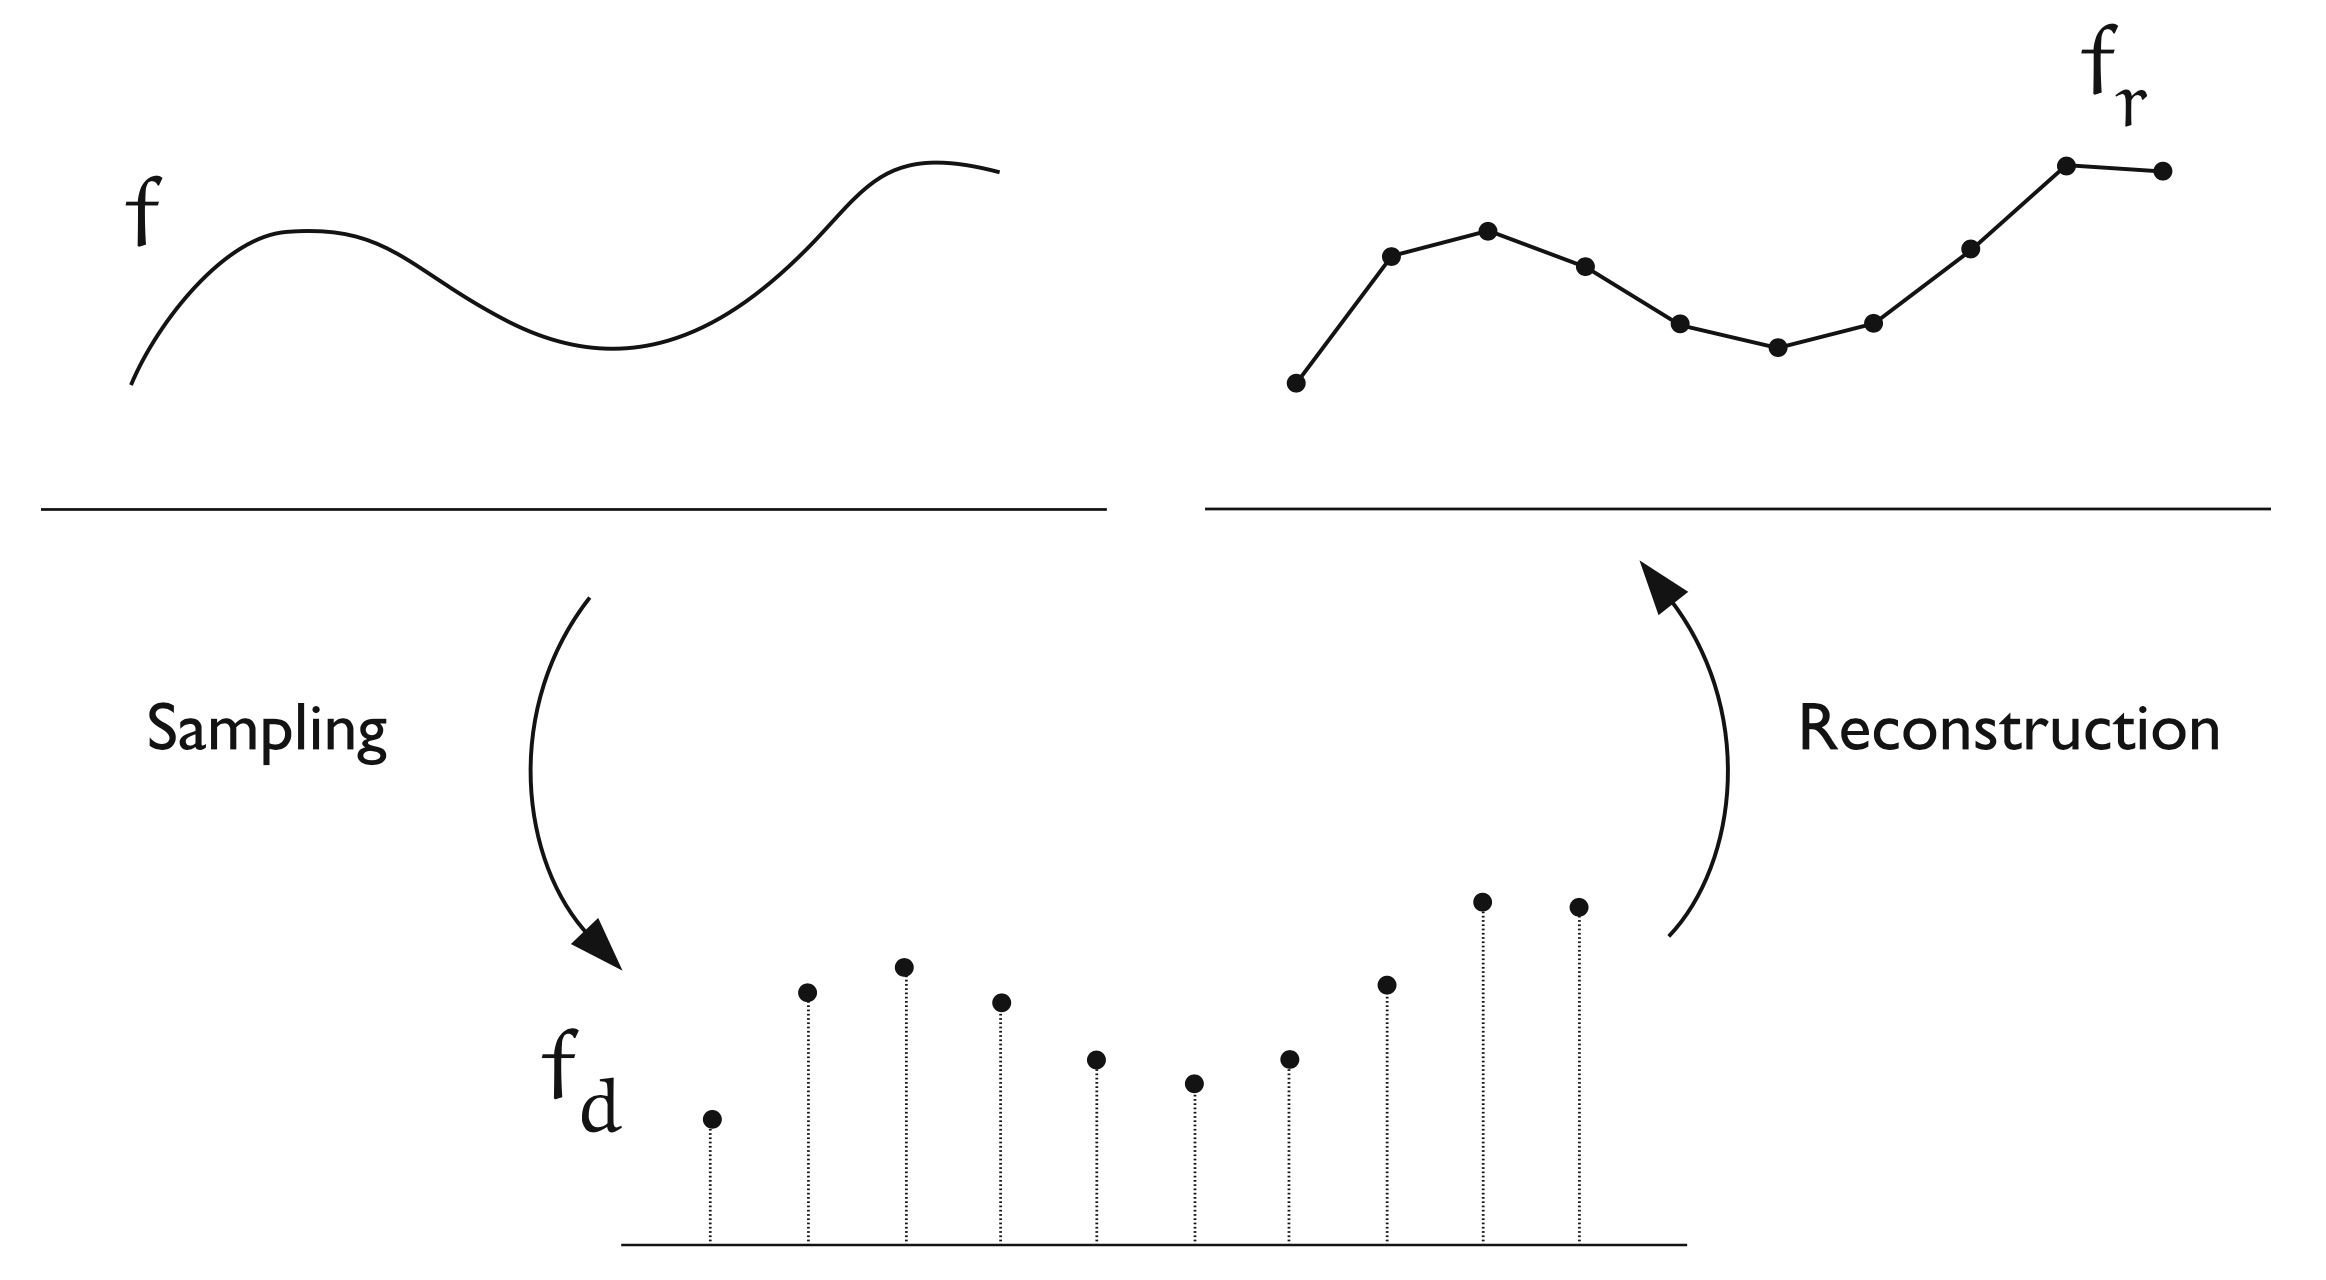
\includegraphics[width=0.85\linewidth]{img/ch2/sampling-reconstruction.png}
  \caption{Illustration of sampling and reconstruction processes.}
  \label{f:sampling-reconstuction}
\end{figure}


One of the fundamental results in this area is the \textbf{Shannon-Nyquist Sampling Theorem} \cite{Shannon1949}. This theorem asserts that a continuous-time, band-limited signal can be perfectly reconstructed from its samples, provided that the sampling rate is at least twice the highest frequency present in the signal. Formally, for a continuous-time signal \( x(t) \) with a maximum frequency component of \( B \) Hz, perfect reconstruction is possible if the sampling frequency \( F_s \) satisfies:
\[
F_s \geq 2B
\]
This critical threshold, \( 2B \), is known as the **Nyquist frequency**.

- \( F_s \): Sampling frequency (in samples per second)
- \( B \): Maximum frequency of the signal (in Hz)

The theorem is central to digital signal processing, as it guarantees that a sufficiently sampled signal retains all the information of its continuous counterpart.

When the sampling frequency falls below the Nyquist limit, \textbf{aliasing} occurs. Aliasing is a form of signal distortion where higher frequency components are misrepresented as lower frequencies in the discrete signal. This distortion results in an inaccurate and misleading reconstruction of the original signal, as illustrated in Figure \ref{f:aliasing-example}.

\begin{figure}[!h]
  \centering
  
\includegraphics[width=0.85\linewidth]{img/placeholder512.png}
  \caption{Illustration of Aliasing.}
  \label{f:aliasing-example}
\end{figure}

The Shannon-Nyquist theorem applies to \textbf{band-limited} signals—those whose frequency content is confined within a finite range. If a signal contains infinite frequency components, no finite sampling rate can fully capture its information. In such cases, even a high sampling rate would still result in aliasing, as the unbounded frequency components would fold into the baseband and distort the signal during reconstruction.

The process of signal reconstruction can be viewed as a form of interpolation. If the sampling adheres to the Nyquist criterion, the continuous signal can be exactly reconstructed using the sinc function as the interpolation kernel. The sinc function is defined as:

\begin{align}
  \text{sinc}(t) = \frac{\sin(\pi t)}{\pi t}
\end{align}

The reconstructed signal is obtained by convolving the discrete samples with the sinc function. In essence, this operation fills in the gaps between sampled points by interpolating based on the sinc kernel. 

**Ideal Interpolation**: The sinc function provides the theoretical basis for perfect interpolation. When applied correctly, it allows for the exact recovery of the original continuous signal from its discrete samples, provided the sampling conditions are met.

However, this ideal reconstruction method is not physically realizable. The sinc function extends to infinity in both directions, making it impractical for real-world implementation. Additionally, the ideal low-pass filter that corresponds to the sinc function features a perfectly sharp cutoff at the Nyquist frequency, which is impossible to achieve due to physical constraints in filtering technology.

In conclusion, while the sinc function and ideal low-pass filter represent theoretical constructs for perfect signal reconstruction, their practical implementation is hindered by real-world limitations. Nonetheless, they serve as benchmarks against which practical signal processing techniques are measured.


% % \red{**Implications for Neural Networks**: Relate these ideas to neural networks and why they struggle to learn high-frequency content.}


\subsection{Frequency Domain Analysis and Fourier Transform}

Any signal can be represented in both its natural domain (such as time or space) and the frequency domain, also known as the spectral domain. The frequency domain provides a powerful framework for analyzing signals by decomposing them into their constituent frequency components. This perspective reveals critical information about the signal's structure, such as its bandwidth, periodicity, and the contribution of different frequencies to the overall signal.

The \textbf{Fourier transform} is the mathematical operation that connects the time or space domain with the frequency domain. It decomposes a signal into a series of sine and cosine waves, each with a specific frequency, amplitude, and phase. For a continuous-time signal \( x(t) \), the Fourier transform \( X(f) \) is defined as:
\[
X(f) = \int_{-\infty}^{\infty} x(t) e^{-j2\pi ft} dt
\]
where:

- \( x(t) \): the time-domain signal,
- \( X(f) \): the frequency-domain representation,
- \( f \): the frequency,
- \( j \): the imaginary unit.

The Fourier transform operates by multiplying the time-domain signal by a complex exponential function for each frequency \( f \) and then integrating the result over all time. This process extracts both the amplitude and phase of each frequency component, revealing the signal's frequency content. By analyzing the frequency spectrum, which consists of the frequencies present in the signal and their associated amplitudes, we can gain insight into the signal's characteristics. 

- **Amplitude**: The amplitude of a frequency component indicates its magnitude or intensity. In the context of audio signals, amplitude corresponds to loudness, while in image processing, it affects brightness or contrast. The amplitude of each frequency component reflects how much that frequency contributes to the overall signal.
  
- **Phase**: The phase represents the initial angle or starting position of the sinusoidal wave at a particular frequency. It determines the relative timing between different frequency components and can affect the overall shape of the signal. Phase shifts can introduce delays or modify the waveform, altering the temporal or spatial structure of the signal.

% % This approach is invaluable in many applications, from audio processing to image analysis and medical imaging, where understanding a signal's frequency content is essential.

The Fourier transform has several forms depending on the nature of the signal. The \textit{continuous Fourier transform} is used for continuous-time signals, while the \textit{discrete Fourier transform} applies to sampled or discrete signals. The \textbf{fast Fourier transform (FFT)} is an efficient algorithm for computing the DFT, enabling real-time signal processing in practical applications.

In the previous section, we discussed how signals are sampled and reconstructed, with particular emphasis on the Shannon-Nyquist sampling theorem and the role of the sinc function in ideal signal reconstruction. The Fourier transform of the sinc function is a rectangular function (Figure \ref{sinc-and-rect}), which highlights a fundamental principle of signal processing: smooth functions in the time domain correspond to compact functions in the frequency domain, and vice versa. The sinc function's Fourier transform being a rectangle in the frequency domain illustrates that it acts as an ideal low-pass filter, passing frequencies within a certain range (the band-limited signal) while cutting off higher frequencies that could lead to aliasing.

\begin{figure}[!h]
  \centering
  
\includegraphics[width=0.85\linewidth]{img/placeholder512.png}
  \caption{Sinc function and its Fourier Transform.}
  \label{f:sinc-and-rect}
\end{figure}

% % The **sinc function**, defined as \( \text{sinc}(t) = \frac{\sin(\pi t)}{\pi t} \), plays a crucial role in both the time and frequency domains. It serves as the ideal interpolation kernel for reconstructing continuous signals from discrete samples, ensuring that no information is lost under perfect conditions. 

The Fourier transform not only allows us to decompose signals into their frequency components but also provides a clear connection between sampling theory and frequency domain analysis. The frequency domain offers an intuitive way to understand the **band-limited nature** of signals: only frequencies below the Nyquist frequency are preserved during sampling. Thus, the Fourier transform gives us the tools to analyze which frequencies are captured and which might cause distortion if undersampled.

% \subsubsection{Inverse Fourier Transform}

The \textbf{inverse Fourier transform} is equally important, as it allows us to reconstruct the original signal from its frequency-domain representation. If we know \( X(f) \), the frequency-domain signal, we can retrieve the time-domain signal \( x(t) \) by applying the inverse Fourier transform:

\[
x(t) = \int_{-\infty}^{\infty} X(f) e^{j2\pi ft} df
\]

This operation restores the original signal by summing all its frequency components (sine and cosine waves) back into the time domain. The inverse Fourier transform provides the foundation for reconstructing signals, just as the sinc function is used in the time domain for ideal interpolation.

Thus, the Fourier transform and its inverse create a bridge between the time and frequency domains, allowing us to switch between these perspectives. When combined with sampling theory, these transformations help us understand how signals can be efficiently represented, manipulated, and reconstructed in both domains.

When signals are sampled, we effectively multiply the original continuous signal by a sequence of Dirac delta functions (impulses). In the frequency domain, this multiplication corresponds to a convolution with a train of impulses, which leads to periodic replicas of the signal's frequency spectrum. This relationship emphasizes the importance of the Nyquist criterion: if the sampling rate is too low (below twice the highest frequency in the signal), these spectral replicas overlap, resulting in aliasing. The Fourier transform enables us to clearly visualize this aliasing effect by showing how undersampling distorts the signal’s frequency content.


% % \red{Visualizing Signals in the Frequency Domain**: Use simple examples (e.g., sine waves) to demonstrate how different frequencies combine to form complex signals.

% % 9. **Stochastic Signals and Noise Models**
% %    - **Introduction to Stochastic Processes**: Briefly explain what stochastic signals are and how they differ from deterministic ones.
% %    - **Perlin Noise and Procedural Patterns**: Use Perlin noise as an example to illustrate how randomness is introduced into signals.
% %    - **Filtering and Noise Removal**: Explain basic techniques for handling noise and filtering in both spatial and spectral domains.

\section{Multiresolution Analysis}

Multiresolution analysis (MRA) offers a hierarchical approach to understanding signals at different levels of detail. By breaking down signals into components that represent varying scales of resolution, MRA helps to capture both global trends and fine details. This technique mimics the way we naturally process visual information, focusing on broader patterns while also perceiving intricate details as needed.

In MRA, signals are decomposed into a coarse approximation, which retains the broader features, and a series of detail coefficients, representing finer, localized features. This approach allows for efficient representation and processing of signals, reducing storage requirements and computational complexity by focusing on the relevant details while discarding less important information.

Multiresolution techniques are widely used in areas such as image processing, signal compression, feature extraction, and wavelet analysis. The following sections provide an overview of two primary methods for multiresolution analysis: pyramids and wavelets.

\subsection{Pyramids: Gaussian and Laplacian}

One of the simplest and most common techniques in MRA is the use of \textit{Gaussian and Laplacian pyramids}. These pyramids represent signals at multiple resolutions, enabling efficient manipulation and analysis across scales.

A \textit{Gaussian pyramid} is built by repeatedly downsampling a signal, typically after applying a low-pass filter to avoid aliasing. At each level, the signal is smoothed using a Gaussian kernel and then reduced in size by subsampling. This results in a pyramid of progressively smaller, coarser versions of the original signal, where each level contains less spatial detail than the previous one.

The mathematical formulation for constructing a Gaussian pyramid is:

\begin{align}
  G_l(x, y) = (G_{l-1}(x, y) * H(x, y)) \downarrow 2
\end{align}

where:
- \( G_l(x, y) \) is the Gaussian pyramid at level \( l \),
- \( H(x, y) \) is a Gaussian low-pass filter, and
- \( \downarrow 2 \) denotes downsampling by a factor of 2.

A \textit{Laplacian pyramid} captures the differences between consecutive levels of the Gaussian pyramid, representing the high-frequency details lost during downsampling. By subtracting the smoothed, downsampled signal from its original form, the Laplacian pyramid isolates these finer details, allowing for a detailed multiscale representation.

The relationship between the Gaussian and Laplacian pyramids is given by:

\begin{align}
  L_l(x, y) = G_{l-1}(x, y) - (G_l(x, y) \uparrow 2 * H(x, y))
\end{align}

where:
- \( L_l(x, y) \) is the Laplacian pyramid at level \( l \),
- \( \uparrow 2 \) denotes upsampling by a factor of 2.

The original signal can be reconstructed from the Laplacian pyramid by iteratively adding the details from each level back to the coarser approximations:

\begin{align}
  G_{l-1}(x, y) = G_l(x, y) \uparrow 2 * H(x, y) + L_l(x, y)  
\end{align}

By progressively adding the finer details back to the lower-resolution versions, the full-resolution signal is restored. In applications such as image compression, storing only the coarse approximation and the detail coefficients leads to efficient data representation.

\subsection{Wavelet Transforms}

While pyramid structures provide a basic form of multiresolution analysis, \textbf{wavelet transforms} offer a more sophisticated and flexible framework. Wavelets differ from pyramids in that they allow for localized, multiresolution analysis in both time (or space) and frequency. This makes them especially useful for signals with transient or localized features.

The key idea behind wavelets is to decompose a signal into a series of \textit{scaled} and \textit{shifted} versions of a fundamental waveform, known as the \textit{mother wavelet}. This process captures both the frequency and location information of the signal components, providing a time-frequency representation that is more adaptive than Fourier-based methods.

In wavelet analysis, a signal is decomposed into approximation coefficients (capturing low-frequency information) and detail coefficients (capturing high-frequency details). This is achieved by convolving the signal with a set of filters: a low-pass filter for approximations and a high-pass filter for details. The decomposition is applied recursively to the approximation coefficients, resulting in a hierarchical, multiresolution representation of the signal.

Mathematically, the wavelet decomposition can be expressed as:

\begin{align}
  A_l = (A_{l-1} * \phi) \downarrow 2, \quad D_l = (A_{l-1} * \psi) \downarrow 2
\end{align}

where:
- \( A_l \) represents the approximation coefficients at level \( l \),
- \( D_l \) represents the detail coefficients,
- \( \phi \) is the scaling function (low-pass filter),
- \( \psi \) is the wavelet function (high-pass filter), and
- \( \downarrow 2 \) denotes downsampling by a factor of 2.

Wavelets naturally offer multiresolution analysis, where larger scales correspond to global features (low-frequency components), and smaller scales capture localized details (high-frequency components). This flexibility allows wavelets to handle signals with varying levels of smoothness or complexity.

The original signal can be reconstructed from its wavelet coefficients by reversing the decomposition process, first upsampling the approximation and detail coefficients, and then applying the inverse filters.

\begin{align}
  A_{l-1} = (A_l \uparrow 2 * \phi) + (D_l \uparrow 2 * \psi)  
\end{align}

This reconstruction process is computationally efficient and forms the basis for many practical applications of wavelets, such as image compression (e.g., JPEG2000), signal denoising, and feature extraction.


\section{Neural Networks}

Artificial Neural networks are computational models inspired by the biological neural networks found in animal brains. These networks consist of interconnected units known as \textbf{artificial neurons}, which simulate the behavior of biological neurons. Each neuron receives inputs, processes them through weighted connections, and produces an output that can be transmitted to other neurons. This architecture allows neural networks to learn complex patterns and relationships within data, making them particularly effective for tasks such as image recognition and natural language processing. In fact, they are universal approximators \red{CITE}.

The fundamental building blocks of a neural network are artificial neurons, which receive inputs represented as real numbers. Each input is associated with a weight that signifies the strength of the connection between neurons. The output of a neuron is calculated as the weighted sum of its inputs plus a bias term, expressed mathematically as:

\[
y = f\left(\sum_{i=1}^{n} w_i x_i + b\right)
\]

where \(y\) is the output, \(w_i\) are the weights, \(x_i\) are the inputs, \(b\) is the bias, and \(f\) is an activation function applied to introduce non-linearity into the model.

Weights are critical parameters that adjust during training to minimize prediction error. Biases allow neurons to shift their activation function, providing additional flexibility in modeling complex relationships. Both weights and biases are updated through optimization algorithms during the training process.

Neural networks learn through a process called \textbf{backpropagation}, which efficiently computes gradients needed for optimization. The learning process involves two main steps: 

\begin{enumerate}
    \item \textbf{Forward Pass}: Inputs are passed through the network to obtain predictions.
    \item \textbf{Backward Pass}: The error between predicted outputs and actual targets is calculated using a loss function (e.g., mean squared error or cross-entropy). The gradients of this error with respect to each weight are computed using the chain rule.
\end{enumerate}

The weights are then updated using an optimization algorithm like \textbf{gradient descent}, which adjusts weights in the direction that minimizes the loss function:

\[
w = w - \eta \nabla L(w)
\]

where \(w\) represents weights, \(\eta\) is the learning rate, and \(\nabla L(w)\) is the gradient of the loss function with respect to weights.

Neural networks can be categorized into \textbf{shallow} and \textbf{deep networks} based on their architecture. A shallow network typically consists of an input layer, one hidden layer, and an output layer. In contrast, deep networks contain multiple hidden layers that enable them to learn hierarchical representations of data. Stacking layers increases the representational power of the network; each additional layer allows the model to capture more complex features from the input data.

In the context of neural networks, \textbf{capacity} refers to the ability of a model to fit a wide variety of functions. It is determined by the architecture of the network, including the number of layers and the number of neurons within those layers. A network with high capacity can learn complex patterns in data, while a network with low capacity may struggle to capture the underlying relationships. The capacity of a neural network is closely linked to its \textbf{expressive power}—the range of functions it can approximate. For instance, a deep neural network with many hidden layers and neurons can represent more intricate functions than a shallow network. However, this increased capacity comes with trade-offs, particularly concerning generalization. A highly expressive model might overfit the training data, learning patterns that do not generalize well to new, unseen data, thus requiring regularization techniques to manage this balance.


Activation functions play a crucial role in determining the output of each neuron by introducing non-linearity into the network. Common activation functions include:

\begin{itemize}
    \item \textbf{Sigmoid}: Maps outputs to a range between 0 and 1.
    \[
    f(x) = \frac{1}{1 + e^{-x}}
    \]
    
    \item \textbf{Hyperbolic Tangent (tanh)}: Maps outputs to a range between -1 and 1.
    \[
    f(x) = \tanh(x) = \frac{e^x - e^{-x}}{e^x + e^{-x}}
    \]
    
    \item \textbf{Rectified Linear Unit (ReLU)}: Outputs zero for negative inputs and linear for positive inputs.
    \[
    f(x) = \max(0, x)
    \]
\end{itemize}

The choice of activation function can significantly impact network performance and convergence during training.

% ---

\subsection{Overfitting and Underfitting}

In the context of neural networks, two important challenges are **overfitting** and **underfitting**. These issues arise from how well the model's capacity aligns with the complexity of the data, and they are closely related to how the model performs on the training set versus unseen test data.

**Underfitting** occurs when the model is too simplistic and lacks the capacity to learn the underlying patterns in the data. This typically happens when the network has too few layers or neurons, preventing it from capturing the complexities within the dataset. As a result, the model fails to perform well on both the training data and the test data, as it cannot even identify the basic trends present in the data. An underfitted model is characterized by poor performance across the board.

On the other hand, **overfitting** happens when the model has excessive capacity, allowing it to memorize the training data instead of generalizing from it. While the model might achieve very low error on the training set, it struggles to handle new, unseen data. This occurs because the overfitted model learns specific details and noise in the training data that don't generalize to broader trends in other datasets. Overfitting leads to a situation where the model's performance on the training data is excellent, but its performance on test data is significantly worse.

Mathematically, these two issues can be observed through the behavior of the loss function. In the case of underfitting, both training loss and validation loss remain high, indicating that the model is not capturing enough of the underlying structure of the data:

\[
\text{High training loss and high validation loss:} \quad L_{\text{train}} \gg 0 \quad \text{and} \quad L_{\text{val}} \gg L_{\text{train}}
\]

For overfitting, the training loss becomes very low, but the validation loss is much higher, reflecting the model's poor generalization to new data:

\[
\text{Low training loss and high validation loss:} \quad L_{\text{train}} \approx 0 \quad \text{and} \quad L_{\text{val}} \gg L_{\text{train}}
\]

To address these challenges, it is essential to find a balance between a model's capacity and its ability to generalize. Several techniques are commonly used to combat overfitting, such as regularization, dropout, and early stopping:

- **Regularization** (e.g., L1 or L2) adds a penalty term to the loss function, discouraging overly complex models by constraining the weights. This helps to reduce overfitting by preventing the model from becoming too specialized to the training data.
  
- **Dropout** involves randomly deactivating a portion of the neurons during training. This technique prevents neurons from relying too heavily on one another, forcing the network to learn more robust features that generalize better.
  
- **Early stopping** monitors the performance of the model on validation data during training and stops the process when performance on the validation set begins to deteriorate, thereby preventing overfitting.

Ultimately, understanding how to manage capacity is crucial in designing neural networks that can learn effectively from training data while also generalizing well to new examples. Achieving the right balance between underfitting and overfitting is essential in many fields, such as computer vision and signal processing, where the accuracy of predictions on unseen data is vital for practical applications.

% ---

\subsection{Coordinate-Based Neural Networks and Implicit Neural Representations}

Coordinate-based neural networks represent a breakthrough in how data is modeled and encoded, especially in spatial domains like images and signals. The central concept is to use neural networks to express data as a continuous function of spatial coordinates. By doing this, various types of signals—such as 2D images or 3D shapes—can be represented by mapping spatial coordinates directly to the corresponding output values, like pixel colors or spatial features.

**Implicit Neural Representations (INRs)** are a specific realization of this idea. Unlike traditional methods that rely on discrete grids (e.g., pixel arrays for images or voxel grids for 3D geometries), INRs treat signals as continuous functions. Rather than storing values at fixed, discrete points, an implicit representation defines a function:

\[
f: \mathbb{R}^n \to \mathbb{R}^m
\]

This function maps any coordinate from an \(n\)-dimensional input space to a corresponding \(m\)-dimensional output value. For instance, in the case of a 2D image, an INR would take a coordinate \((x, y)\) as input and return the RGB color value at that point:

\[
\text{Color} = f(x, y) = (R, G, B)
\]

The advantage of this continuous representation is its flexibility—it is not restricted to any specific spatial resolution. In theory, INRs can achieve infinite resolution, meaning they can be sampled at any desired level of detail without the limitations of traditional discrete grids. This is particularly useful for applications like **super-resolution imaging** or working with high-dimensional datasets.

Furthermore, INRs offer **efficient memory usage**. The memory required to store an implicit representation scales with the complexity of the signal rather than its spatial resolution. For complex datasets, this efficiency is crucial because traditional methods might demand excessive storage, especially when handling high-resolution data.

The impact of implicit neural representations extends far beyond storage optimization. INRs are being utilized in several advanced applications in fields like computer graphics and computer vision:

1. **3D Shape Representation**: INRs can outperform traditional 3D shape representations such as meshes or point clouds. By learning continuous functions over geometric shapes, they allow for seamless deep learning-based modeling of shape priors.

2. **Signal Reconstruction**: INRs can be used to reconstruct missing or incomplete data in signals. For example, given a sparse set of image pixels or audio data points, the learned function can fill in the gaps, making INRs particularly valuable in scenarios where the input data is noisy or incomplete.

3. **Solving Partial Differential Equations (PDEs)**: Some architectures, like **Sinusoidal Representation Networks (SIRENs)**, leverage periodic activation functions such as sine functions. This choice of activations enhances the network’s ability to model complex signals, including their derivatives, making SIRENs especially suitable for solving boundary value problems associated with PDEs. The periodic nature of the activations provides an ideal framework for capturing the oscillatory behavior of solutions to such equations.

Thus, coordinate-based neural networks and implicit neural representations represent a paradigm shift in how we approach and process spatial data. By conceptualizing signals as continuous functions instead of discrete samples, these models provide enhanced flexibility, efficiency, and power in representing complex datasets. As research in this area continues to advance, these approaches are likely to drive further innovations across a range of applications, from computer vision to graphics and beyond.

% % Citations:
% % [1] https://github.com/vsitzmann/awesome-implicit-representations
% % [2] https://www.vincentsitzmann.com/siren/
% % [3] https://www.reddit.com/r/MLQuestions/comments/qta8v6/could_someone_explain_what_an_implicit_neural/
% % [4] https://en.wikipedia.org/wiki/Neural_network_(machine_learning)
% % [5] https://aws.amazon.com/what-is/neural-network/
% % [6] https://www.science-on-stage.eu/machine-learning/neurons
% % [7] https://eitca.org/artificial-intelligence/eitc-ai-dltf-deep-learning-with-tensorflow/introduction-eitc-ai-dltf-deep-learning-with-tensorflow/introduction-to-deep-learning-with-neural-networks-and-tensorflow/examination-review-introduction-to-deep-learning-with-neural-networks-and-tensorflow/what-are-the-key-components-of-a-neural-network-and-what-is-their-role/
% % [8] https://en.wikipedia.org/wiki/Artificial_neuron



\subsection{Sinusoidal Neural Networks}

Sinusoidal neural networks leverage sine functions as activation functions, offering a powerful way to model signals with intricate details. The motivation for using sine functions lies in their ability to capture fine variations in data, making them particularly well-suited for representing high-frequency components of signals. In contrast to conventional neural networks that use activation functions like ReLU or sigmoid, sinusoidal networks are designed to approximate complex signals more naturally, especially those characterized by oscillations and periodic patterns.

The use of sine functions allows sinusoidal neural networks to represent signals in both the **spatial** and **frequency** domains. Signals, especially those in fields such as audio, image processing, and computer graphics, often contain fine structures that require high-frequency components for accurate representation. A sinusoidal activation function, defined as:

\[
\sigma(x) = \sin(x)
\]

is inherently capable of generating oscillations. These oscillations enable the network to capture fine variations in data, something that traditional activations might struggle with. This characteristic makes sinusoidal neural networks ideal for tasks where precision at smaller scales is critical, such as super-resolution, texture generation, or even physics simulations.

The relationship between sinusoidal networks and the **frequency domain** is central to understanding their expressive power. In signal processing, the **Fourier series** is a method for expressing a periodic function as a sum of sine and cosine terms, each associated with a specific frequency. A signal \(f(x)\) can be decomposed into a sum of sinusoids as:

\[
f(x) = a_0 + \sum_{n=1}^{\infty} \left( a_n \cos(n x) + b_n \sin(n x) \right)
\]

This decomposition reveals that any periodic signal can be described as a combination of sinusoids of different frequencies. By using sine functions as activations, sinusoidal neural networks can directly represent the frequency components of a signal, offering the ability to capture both low-frequency (coarse) and high-frequency (fine) details. This is particularly useful when modeling signals that vary at multiple scales, as the network can flexibly adapt to different frequency ranges.

**Sinusoidal Representation Networks (SIREN)** are a specific type of neural network that employ sine functions as their core activations. Introduced as an alternative to traditional architectures, SIRENs have shown significant advantages in representing complex signals, particularly in the context of continuous signals such as images, 3D shapes, and physical fields.

A SIREN architecture typically defines each layer of the network as:

\[
y = \sin(Wx + b)
\]

where \(W\) represents the weight matrix, \(x\) is the input, and \(b\) is the bias term. The sine activation allows the network to approximate high-frequency components, which is especially beneficial for tasks like **implicit neural representation** (as discussed previously) and **solving partial differential equations (PDEs)**.

% Advantages of SIREN

% 1. **Modeling Fine Details**: SIRENs excel at capturing fine details and sharp transitions in signals due to the periodic nature of sine functions. This makes them highly effective in applications such as super-resolution imaging, surface reconstruction, and neural rendering.

% 2. **Smooth Representations**: The continuous nature of the sine function ensures that the output of SIRENs is inherently smooth. This property is particularly useful in applications where smoothness and differentiability of the output are required, such as modeling surfaces or fields in 3D space.

% 3. **Efficient Frequency Control**: SIRENs can naturally control the frequency of their output, allowing them to capture both coarse structures and intricate high-frequency details. This multi-resolution capability is a key advantage over conventional neural networks, which may require additional architectural components (e.g., skip connections) to handle multi-scale data effectively.

% Challenges of SIREN

% While SIRENs offer substantial benefits, they also present some unique challenges:

% 1. **Training Stability**: The use of sine activations can lead to instabilities during training, particularly when initializing the weights. If not properly initialized, the network may struggle to converge or produce overly oscillatory outputs. To address this, specific weight initialization strategies, such as **periodic weight scaling**, are often required.

% 2. **Generalization to Low Frequencies**: While SIRENs excel at high-frequency signal approximation, they may struggle to represent low-frequency components effectively. This issue arises because the network is more naturally attuned to oscillatory patterns, which can lead to difficulties when modeling smoother, broader trends in the data.

% 3. **Complexity of Derivatives**: Another challenge comes from the fact that, while sine functions are smooth and differentiable, the resulting derivatives may be complex to compute efficiently for certain high-dimensional tasks, such as solving higher-order PDEs.

% Conclusion

% Sinusoidal neural networks, and particularly SIRENs, represent a powerful framework for modeling signals that contain intricate, high-frequency components. By leveraging sine functions as activations, these networks can capture fine details that are often missed by traditional architectures. While they offer distinct advantages in precision and smoothness, their unique challenges—such as training instability and generalization to low-frequency signals—require careful consideration when applied in practice. Despite these challenges, SIRENs continue to push the boundaries of neural network-based representations in fields like computer vision, graphics, and scientific computing.


% \subsection{Sinusoidal Neural Networks}

% Sinusoidal neural networks, particularly exemplified by **Sinusoidal Representation Networks (SIRENs)**, utilize sine functions as activation functions to effectively model complex signals. The choice of sine functions is grounded in their unique properties that allow these networks to capture fine details and represent intricate spatial patterns. Unlike traditional activation functions like ReLU or tanh, sine functions are periodic and smooth, which is crucial for modeling signals that exhibit oscillatory behavior or require high-frequency detail.

% #### Capturing Fine Details

% The periodic nature of sine functions enables sinusoidal networks to approximate signals with high fidelity. This capability is particularly beneficial in applications involving natural signals, such as images and audio, where fine details are essential for accurate representation. The smoothness of sine functions allows these networks to maintain continuity and differentiability, which is vital when modeling physical phenomena governed by partial differential equations (PDEs). 

% By employing sine activations, SIRENs can effectively represent a signal's derivatives, which are often critical in understanding the underlying dynamics of the data being modeled. This characteristic makes them suitable for solving boundary value problems, such as the Poisson equation or the Helmholtz equation, where precise control over spatial and temporal derivatives is necessary.

% #### Frequency Domain Representation

% The link between sinusoidal activations and Fourier series further elucidates their effectiveness in signal representation. Fourier series express periodic functions as sums of sine and cosine terms, allowing for the decomposition of signals into their frequency components. In this context, sinusoidal neural networks can be viewed as approximating a function through a harmonic sum:

% $$
% f(x) = \sum_{n=0}^{N} a_n \sin(b_n x + \phi_n)
% $$

% where $$a_n$$, $$b_n$$, and $$\phi_n$$ represent the amplitude, frequency, and phase shift of each harmonic component. This formulation highlights how SIRENs can leverage the properties of sine functions to capture both low-frequency trends and high-frequency details in a unified framework.

% #### Overview of Sinusoidal Representation Networks (SIREN)

% SIRENs are designed specifically to harness the advantages of sinusoidal activations for implicit neural representations. They consist of multiple layers where each layer applies a sine activation function to its outputs. This architecture allows SIRENs to model complex natural signals while maintaining smoothness and continuity across the representation.

% One of the key advantages of SIRENs is their ability to represent signals at varying resolutions without being constrained by traditional grid-based representations. This flexibility enables them to achieve high fidelity in tasks such as image synthesis, 3D shape representation, and audio signal modeling. Additionally, SIRENs have demonstrated superior performance in reconstructing signals from sparse data compared to conventional neural architectures.

% However, training SIRENs presents unique challenges. The periodic nature of sine functions can lead to difficulties in convergence during optimization due to the presence of multiple local minima in the loss landscape. To address this issue, effective initialization schemes are crucial for ensuring stability during training. These schemes help guide the optimization process toward regions of the parameter space that facilitate learning.

% In summary, sinusoidal neural networks leverage the properties of sine functions to provide robust representations of complex signals. Their ability to capture fine details through smoothness and periodicity makes them particularly well-suited for applications that require high precision in modeling physical phenomena. As research continues to advance in this area, SIRENs stand out as a powerful tool for bridging the gap between spatial and frequency domain representations in various fields such as computer graphics, audio processing, and beyond.

% Citations:
% [1] https://docs.siml.ai/creating-a-simulator/neural-network-node/sinusoidal-representation-network
% [2] https://arxiv.org/abs/2212.01833
% [3] https://www.vincentsitzmann.com/siren/
% [4] https://openreview.net/pdf?id=Sks3zF9eg
% [5] https://arxiv.org/abs/2109.09338v2
% [6] https://www.visgraf.impa.br/Data/RefBib/PS_PDF/mrnet-cag-2023/MRNet_CAG-2023.pdf
% [7] https://towardsdatascience.com/sinusoidal-neural-networks-for-digit-classification-bd2b14e57ad8
% [8] https://www.reddit.com/r/MLQuestions/comments/qta8v6/could_someone_explain_what_an_implicit_neural/ % Theoretical Framework

\chapter{Frequency Dynamics in Sinusoidal Neural Networks}
\label{chap:sinusoidal}

In this chapter, we explore the frequency dynamics within sinusoidal neural networks, laying the groundwork for designing architectures that can represent signals across multiple resolutions. While much of the research on sinusoidal neural networks has focused on their capacity to capture high-frequency details, the interplay between frequency initialization, network structure, and learned representations is still not fully understood. Our goal is to analyze these factors systematically and establish a deeper understanding of how frequency components propagate and interact in both shallow and deep sinusoidal architectures.

We initially focus on representing one-dimensional signals using sinusoidal neural networks. This approach allows us to experiment on the control of signal frequencies, visualize them through their Fast Fourier Transform (FFT) plots, and validate our results against classical sampling theory. We progressively increase the complexity of our experiments to evaluate how different initializations and network capacities affect frequency learning.

In our experiments, we employ the Sinusoidal Representation Networks (SIREN) framework (\cite{sitzmann2019siren}) due to its effectiveness in capturing high-frequency signal details and modeling signal derivatives. We conduct an in-depth investigation of its initialization, examining the relationship between the network’s hyperparameters, the inherent frequencies of the input signal, and the frequencies the network learns. Through controlled experiments, we show how the number of neurons, network depth, and specific initialization strategies influence the network's capacity to isolate and reconstruct distinct frequency bands. This analysis allows us to define methods for frequency band filtering and representation by strategically adjusting network width, depth, and weight initialization. These insights will be explored in the design of the MR-Net, a family of neural network architectures presented in Chapter \ref{chap:mr_snn}.


\section{Related Works}

Our focus lies on signals as media objects, usually represented by functions in one, two, and three dimensions. \cite{tancik2020fourfeat} demonstrated, both theoretically and empirically, that standard Multilayer Perceptrons (MLPs) struggle to learn high frequencies in such domains, which are considered low-dimensional domains for machine learning applications. They proposed using Fourier feature mapping to transform input coordinates into a higher-dimensional spectral feature space before processing them through the network. This enables coordinate-based MLPs to effectively capture high-frequency content in low-dimensional signals, overcoming this \textit{spectral bias} (\cite{rahaman2018spectral}).

Sinusoidal neural networks represent a class of coordinate-based networks that employs the sine function as their activation function. They serve as a bridge between spatial and spectral domains due to the close relationship between the sine function and the Fourier basis. The first layer of a sinusoidal neural network projects the signal into spectral space, while the last layer reconstructs the signal from a dictionary of spectral atoms. This characteristic allows them to naturally overcome the spectral bias of regular MLPs. However, these sinusoidal neural networks have been regarded as difficult to train \cite{taming2017}. To address this issue, Sitzmann et al. \cite{sitzmann2019siren} proposed SIREN, a sinusoidal network for signal representation. One of its key contributions is an initialization scheme that ensures stability and convergence, enabling the modeling of fine details consistent with the signal’s frequency content.

The challenge in training sinusoidal neural networks comes in part from the composition of sinusoidal functions, which can generate multiple new and higher frequencies. \cite{novello2022understanding} studied sinusoidal MLPs by expanding them as harmonic sums, demonstrating how numerous new frequencies are expressed as integer linear combinations of the input frequencies. This work provides theoretical justification for sinusoidal MLPs compactness property and contributes to a better understanding of these networks’ behavior.

A simpler form of sinusoidal networks is the Multiplicative Filter Network (MFN) \cite{fathony2020multiplicative}, which can be viewed as a shallow sinusoidal MLP. By using the Hadamard product of matrices instead of standard matrix multiplication, the MFN avoids the composition of sine functions, allowing its representation to be expressed as a closed-form finite sum of sines using basic trigonometric identities. However, despite having a straightforward mechanism to target specific frequency bands, shallow networks like the MFN require significantly more parameters to accurately represent a signal as we will see in the next sections.

% Sinusoidal neural networks have found applications in various fields. 
% % due to their ability to represent high-frequency details and model complex signals. 
% In computer graphics, they are used for tasks such as neural rendering, where they efficiently encode fine geometric and texture details for 3D shapes and scenes (\cite{mildenhall2020nerf, sitzmann2019siren}). In computational imaging, they serve as implicit neural representations for super-resolution, image inpainting, and view synthesis, capturing intricate patterns and producing photorealistic results (\cite{tancik2020fourfeat, park2019deepsdf}). Additionally, sinusoidal networks are employed in physics-informed neural networks (PINNs) for solving partial differential equations, where the smooth periodic activations facilitate modeling complex boundary conditions and solutions (\cite{raissi2019pinns, wang2021eigenvector}). Their versatility also extends to audio signal processing and material modeling, enabling applications like sound synthesis, wave propagation simulation, and compact representations of spatially varying materials (\cite{stich2020audio, bi2020neural}). These networks' ability to seamlessly traverse between spatial and spectral domains makes them powerful tools for any application that demands high-fidelity signal representation.

% Recent advancements like sinusoidal positional encoding (SPE) address challenges in efficiently learning adaptive frequency features without manual tuning 


\section{Frequency Initialization}

The correct initialization of sinusoidal neural networks is critical for having stability during training and convergence to the expected result. According to \cite{sitzmann2019siren}, a SIREN model must be initialized so that for a uniform input in $[-1, 1]$ the outputs of each hidden layer before the sine nonlinearity are standard normal distributed. 

Moreover, the authors of SIREN propose to initialize the first layer of the network so that the sine function $\sin(\omega_0 \cdot W x + b)$ spans multiple periods over $[-1, 1]$. They introduce $\omega_0$ as a hyperparameter that could be adjusted to each signal, while $W$ and $b$ are the weights and biases of a layer in the network. For the examples presented in their work, they used a fixed $\omega_0=30$ and found it to work well empirically, but they did not dive deeper on the \emph{why}.

% The authors of SIREN suggest initializing the first layer of the network to ensure that the sine function \(\sin(\omega_0 \cdot Wx + b)\) spans multiple periods over \([-1, 1]\). They introduce \(\omega_0\) as a hyperparameter that can be adjusted for each signal. Empirically, they found a fixed \(\omega_0 = 30\) to work well, although they do not delve into the underlying reasons.

% In this section, we show how the choice of $\omega_0$  impacts the frequencies learned by the network, the speed of the training and even if it will converge to a reasonable result or collapse into noise. The hyperparameter $\omega_0$ is directly related to the interval of frequencies used to initialize the first layer of the network, determining the set of the spectral atoms where the signal will be projected. This same hyperparameter is also applied on the initialization of the hidden layers as the authors argue it boosts the gradients during the training and accelerates the convergence. However, in the hidden layers, it is basically used as pre-conditioner, a numeral trick, since the implementation multiplies by $\omega_0$ and also divides by this same value. We propose to call this hyperparameter in the hidden layers by $\omega_h$, and keep $\omega_0$ only for the first layer.

In this section, we examine how the choice of \(\omega_0\) impacts the frequencies learned by the network, the speed of training, and whether the network will converge to a reasonable result or collapse into noise. We show that the hyperparameter \(\omega_0\) directly influences the range of frequencies used to initialize the first layer of the network, thus determining the set of spectral atoms onto which the signal will be projected. 

The $\omega_0$ hyperparameter is also applied to the initialization of the hidden layers, as the authors argue that it boosts gradients during training and accelerates convergence. However, in the hidden layers, \(\omega_0\) functions primarily as a pre-conditioner, a numerical trick, since the implementation multiplies the weights by \(\omega_0\) and then divides them by the same value. To clarify this distinction, we propose referring to the hyperparameter in the hidden layers as \(\omega_h\), reserving \(\omega_0\) exclusively for the first layer. In all experiments, the hyperparameter $\omega_h$ will be kept constant equal 30 unless explicitly stated on contrary.

By understanding and adjusting \(\omega_0\), we aim to optimize the training process of sinusoidal neural networks and develop mechanisms for controlled frequency learning.


\subsection{Isolating Frequencies}

A shallow network with just one layer of sinusoidal activation functions can filter a signal by band-limiting its frequency content. Thus, it provides a tool for controlling the level of detail of the output signal. This conclusion is natural since the resulting signal representation is a linear combination of sinusoidal functions with induced frequency band. In a sense, a shallow network is projecting the input signal into a learned dictionary of spectral atoms, then reconstructing it by a linear combination of these atoms, where the weights are also learned.

In that context, a one-layer SIREN network could also be used as a spectral filter, just as in the MFN-based architectures (\cite{fathony2020multiplicative}). To verify this hypothesis, we trained a shallow SIREN controlling the initialization of the weights of the first linear transformation, and observed how this can determine the final reconstruction. In the first experiment, the input signal, presented in Figure \ref{fig:gt-4freqs}, is a combination of four tones, two with lower frequencies (2Hz and 5Hz) and two more with higher frequencies (31Hz and 42Hz). The hyperparameters of the network and the training are sample size: 512; hidden layers: 0; total steps: 200; learning rate: $10^{-2}$; optimization method: Adam; number of neurons: 64 per layer. 

First, we tried to recover the lower frequencies using $\omega_0=10$. The reconstructed signal, displayed in Figure \ref{fig:rec-naive-w0}, resembles a very low-frequency signal. In fact, the Fast Fourier Transform (FFT) of both signals (Figure \ref{fig:fft-smooth-4freqs}) reveals that the network only captured a peak at 2 Hz and learned only small amplitudes of other low frequencies, representing a heavily smoothed version of the input signal.

\begin{figure}[h!]
    \centering
    \begin{subfigure}[b]{0.32\textwidth}
        \centering
        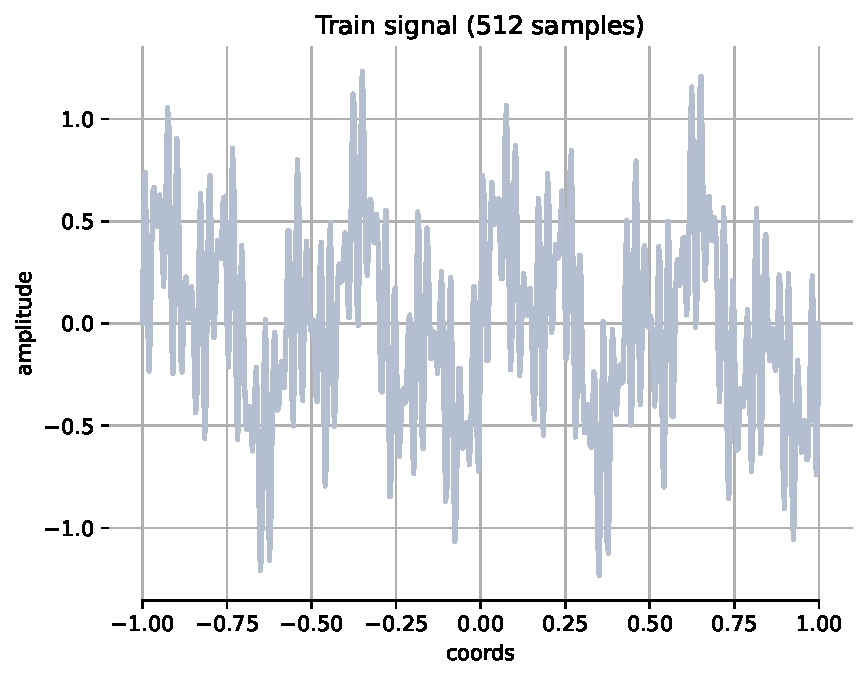
\includegraphics[width=\textwidth]{img/ch3/train_tones512.pdf}
        \caption{Input signal}
        \label{fig:gt-4freqs}
    \end{subfigure}
    \hfill
    \begin{subfigure}[b]{0.32\textwidth}
        \centering
        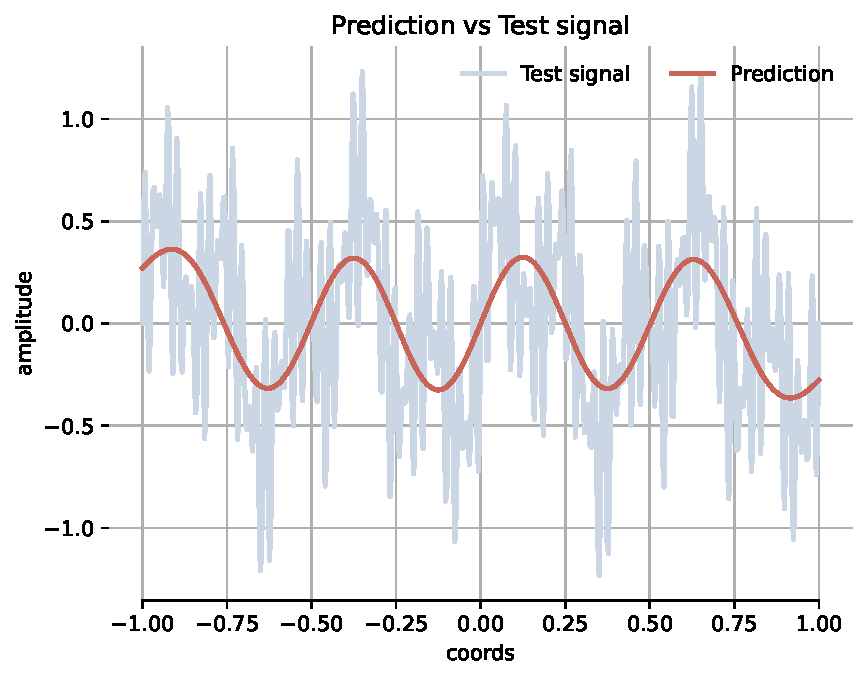
\includegraphics[width=\textwidth]{img/ch3/prediction_w10_smoothed.pdf}
        \caption{Reconstruction}
        \label{fig:rec-naive-w0}
    \end{subfigure}
    \hfill
    \begin{subfigure}[b]{0.32\textwidth}
        \centering
        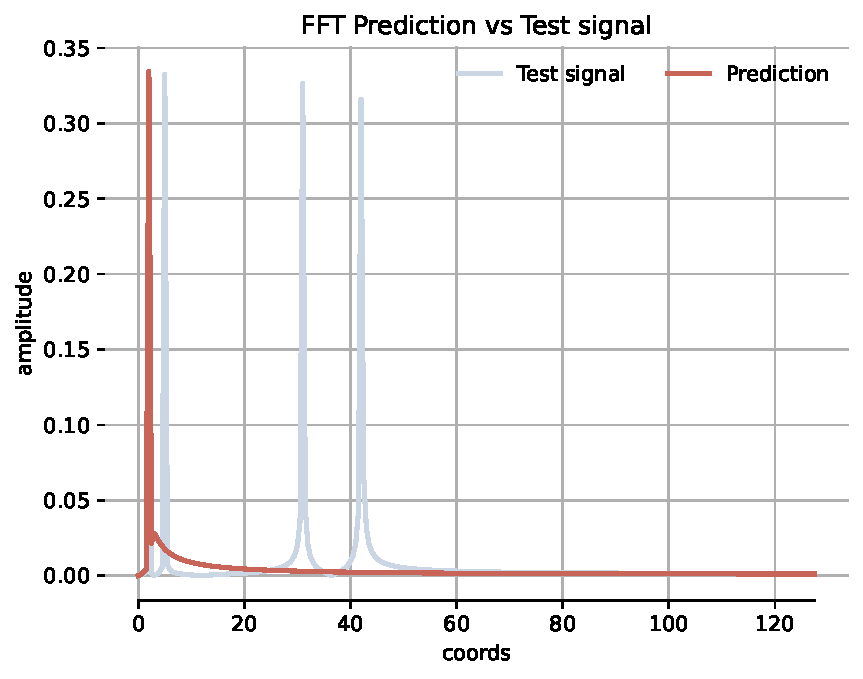
\includegraphics[width=\textwidth]{img/ch3/fft_w10_smoothed.pdf}
        \caption{Frequencies (FFT)}
        \label{fig:fft-smooth-4freqs}
    \end{subfigure}
    \label{f:4freqs-smoothed-reconstruction}
    \caption{Reconstruction of a signal with selected low and high frequencies using a network initialized with very low frequencies.}
\end{figure}


We believe this result is due to the network being initialized with frequencies lower than those present in the signal. Given that the sine function is periodic with a period of $2\pi$, we propose that the hyperparameter $\omega_0$ should always be multiplied by $2\pi$ to better establish a relationship between the initialization of the network's first layer and the range of frequencies represented by each atom in this layer.

Repeating the experiment with $\omega_0 = 10$ Hz, that is $10*2\pi$, we observe the expected behavior: the predicted wave in Figure \ref{fig:rec-2pi-w0} approximates the low-frequency portion of the signal. Notice how the FFT plot (Figure \ref{fig:fft-low-4freqs}) matches the peaks at 2 Hz and 5Hz, while the high frequency tones are not learned.

\begin{figure}[h!]
    \centering
    \begin{subfigure}[b]{0.38\textwidth}
        \centering
        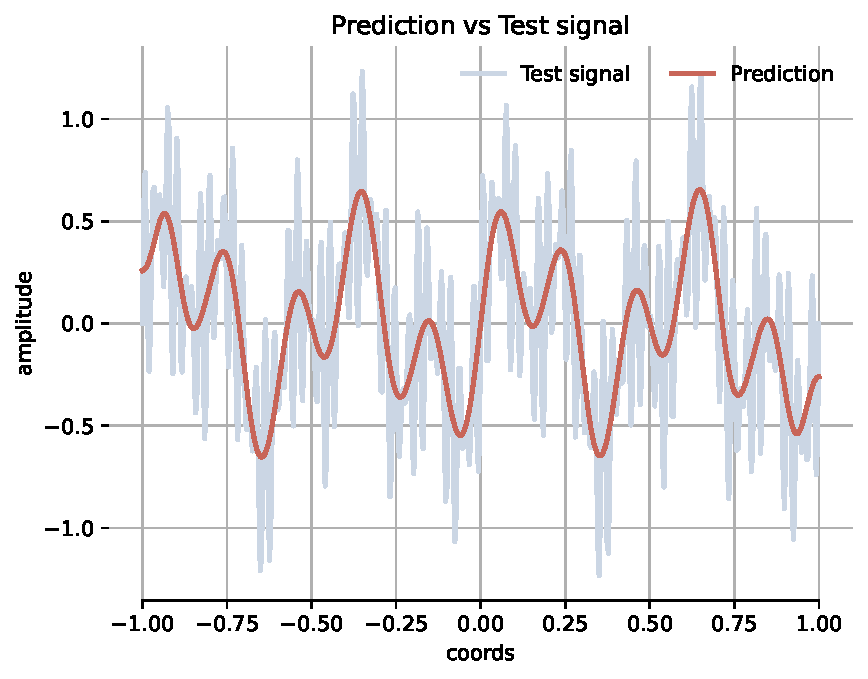
\includegraphics[width=\textwidth]{img/ch3/prediction_w0_2pi.pdf}
        \caption{Reconstruction}
        \label{fig:rec-2pi-w0}
    \end{subfigure}
    % \hfill
    \begin{subfigure}[b]{0.38\textwidth}
        \centering
        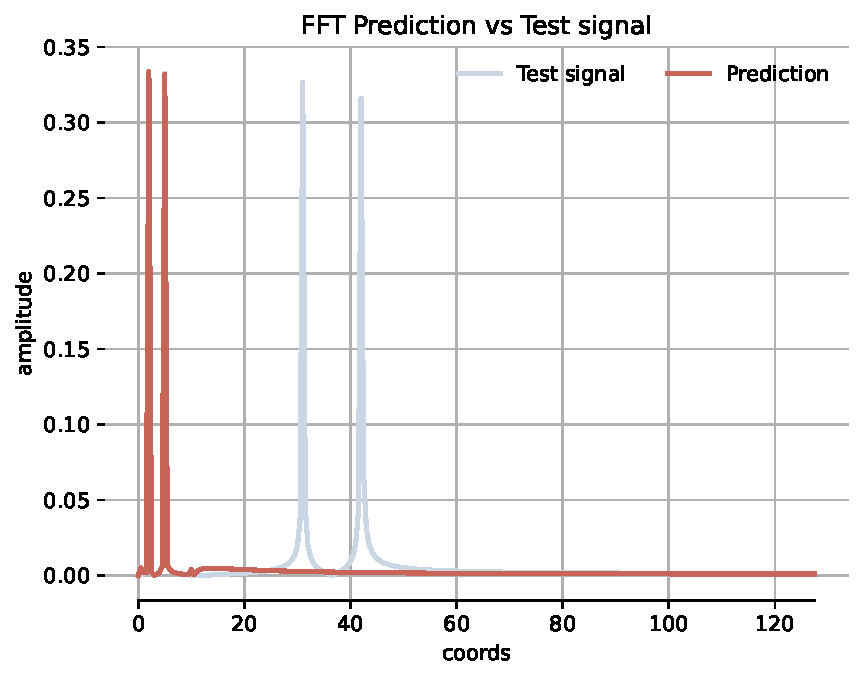
\includegraphics[width=\textwidth]{img/ch3/fft_w0_2pi.pdf}
        \caption{Frequencies (FFT)}
        \label{fig:fft-low-4freqs}
    \end{subfigure}
    \label{f:4freqs-low-reconstruction}
    \caption{Reconstruction of a signal with selected low and high frequencies, where the lower frequencies fall within the initialization range of the network's first layer.}
\end{figure}

Next we change the initialization of the network to frequencies between 25 and 45 Hz. As expected, that also succeeds in predicting the high-frequency tones but fails in capturing the low-frequency ones (Figures \ref{fig:rec-25-45} and \ref{fig:fft-25-45}). Moreover, by initializing the frequencies between 35 and 45 Hz, we are able to isolate the 42 Hz tone (Figures \ref{fig:rec-35-45} and \ref{fig:fft-35-45}).

\begin{figure}[h!]
    \centering
    \begin{subfigure}[b]{0.38\textwidth}
        \centering
        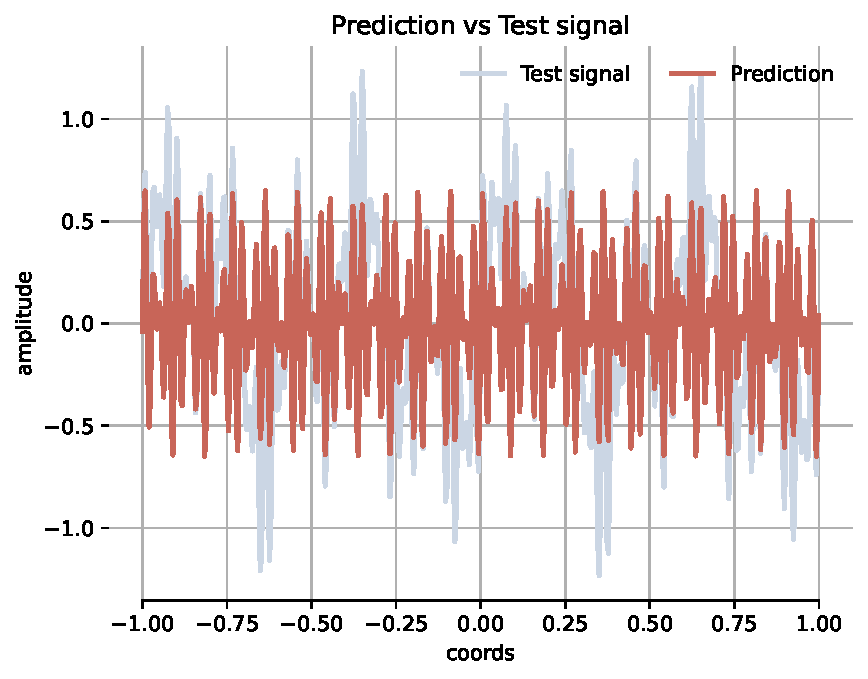
\includegraphics[width=\textwidth]{img/ch3/prediction_w25-45_2pi.pdf}
        \caption{$\omega_0 \in [25, 45]$Hz}
        \label{fig:rec-25-45}
    \end{subfigure}
    % \hfill
    \begin{subfigure}[b]{0.38\textwidth}
        \centering
        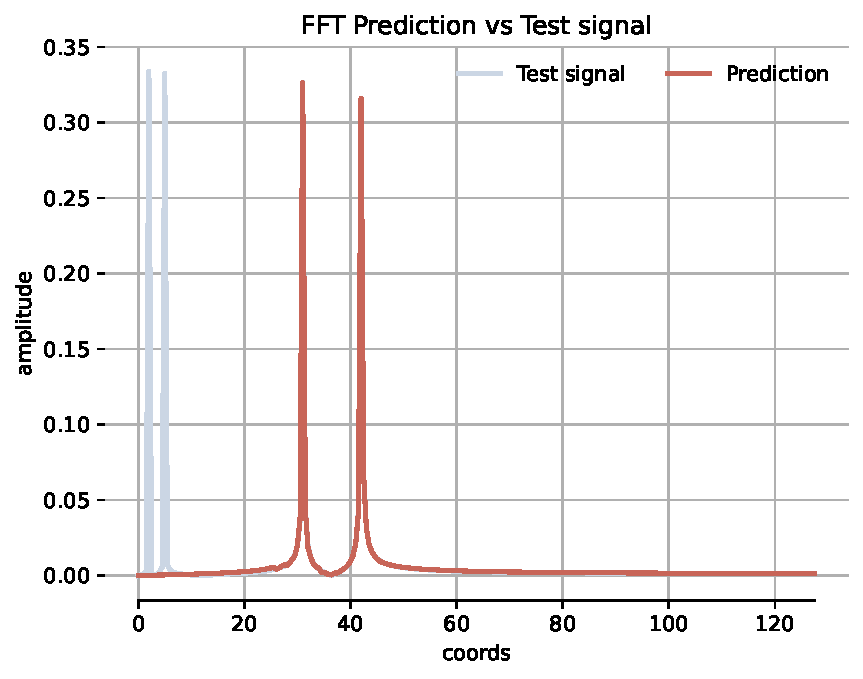
\includegraphics[width=\textwidth]{img/ch3/fft_w25-45.pdf}
        \caption{$\omega_0 \in [25, 45]$Hz}
        \label{fig:fft-25-45}
    \end{subfigure}
    \begin{subfigure}[b]{0.38\textwidth}
        \centering
        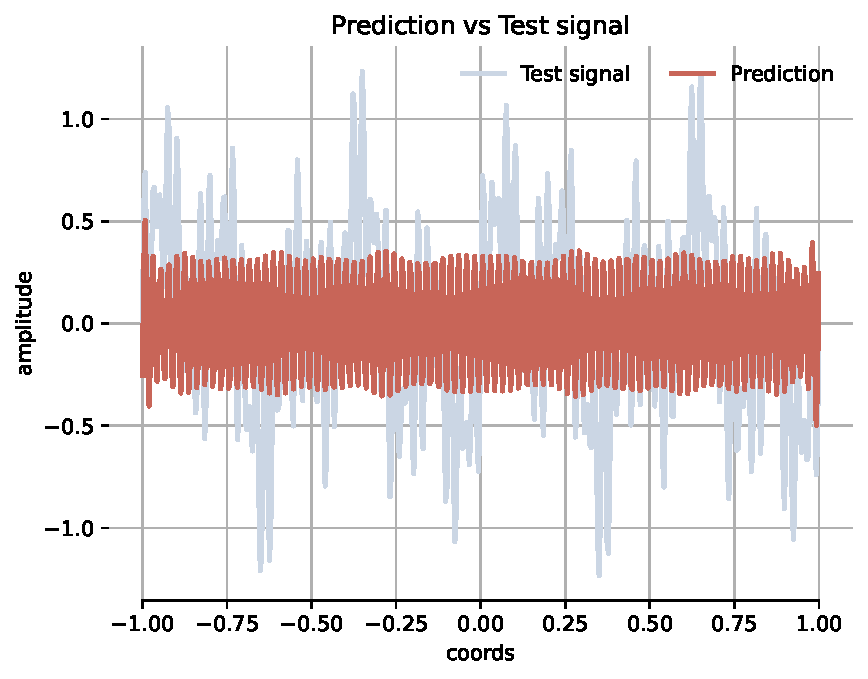
\includegraphics[width=\textwidth]{img/ch3/prediction_w35-45.pdf}
        \caption{$\omega_0 \in [35, 45]$Hz}
        \label{fig:rec-35-45}
    \end{subfigure}
    % \hfill
    \begin{subfigure}[b]{0.38\textwidth}
        \centering
        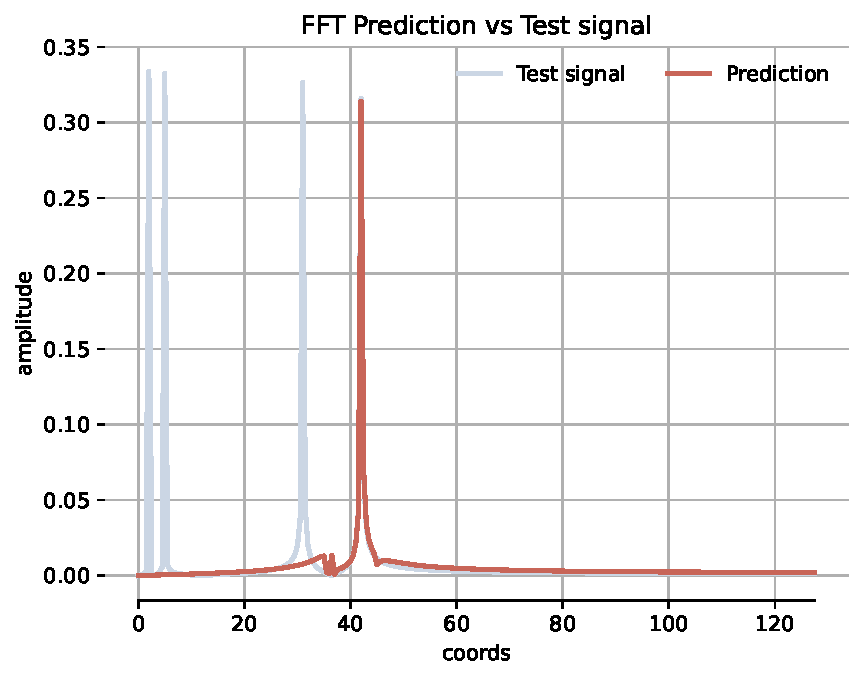
\includegraphics[width=\textwidth]{img/ch3/fft_w35-45.pdf}
        \caption{$\omega_0 \in [35, 45]$Hz}
        \label{fig:fft-35-45}
    \end{subfigure}
    \label{f:high-freqs-reconstruction}
    \caption{Reconstruction of the signal where only the higher frequencies fall within the initialization range of the network’s first layer.}
\end{figure}

Surprisingly, when we use a range of frequencies that encompasses all frequencies present in the input signal, for example $\omega_0 \in [-45, 45]$ Hz, the network does not perfectly fit the signal (Figure \ref{fig:rec-64-full-45}), and a mismatch between the frequencies of the network and those of the input signal is evident in the FFT plot (Figure \ref{fig:fft-64-full-45}). Our hypothesis is that this is due to the network's limited representation capacity, as it is a shallow network with only 64 neurons per layer. To test this, we repeated the experiment with larger models. Figures \ref{fig:rec-128-full-45} and \ref{fig:fft-128-full-45} show an improvement when the network width is increased to 128 neurons per layer. Note that with 256 neurons, the network can fit the signal perfectly, at least qualitatively, as the reconstructed signal appears to superimpose on the input signal both in the spatial (Figure \ref{fig:rec-256-full-45}) and the spectral (Figure \ref{fig:fft-256-full-45}) domains.

\begin{figure}[h!]
    \centering
    \begin{subfigure}[b]{0.32\textwidth}
        \centering
        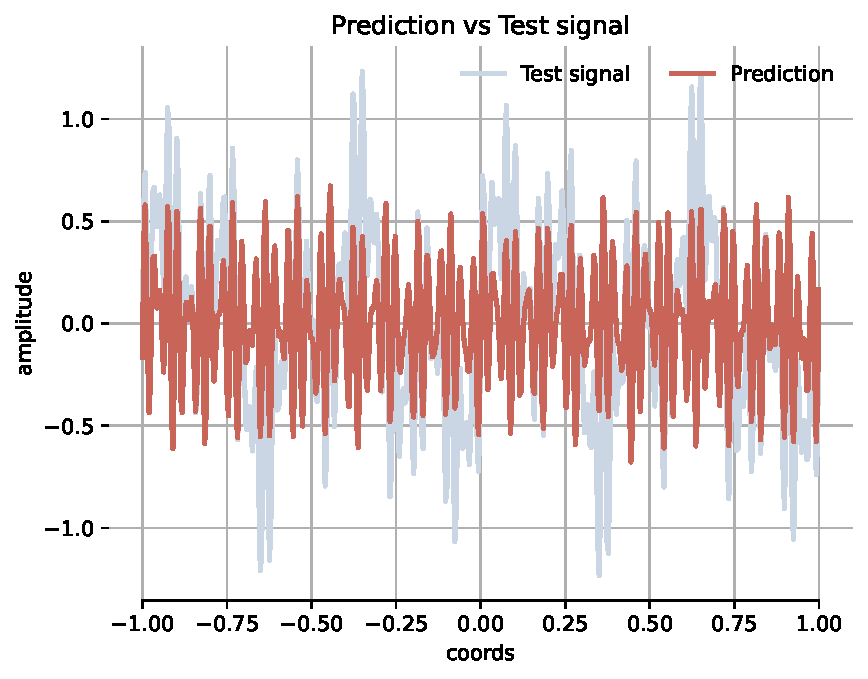
\includegraphics[width=\textwidth]{img/ch3/prediction_w45all_hf64.pdf}
        \caption{64 neurons}
        \label{fig:rec-64-full-45}
    \end{subfigure}
    \hfill
    \begin{subfigure}[b]{0.32\textwidth}
        \centering
        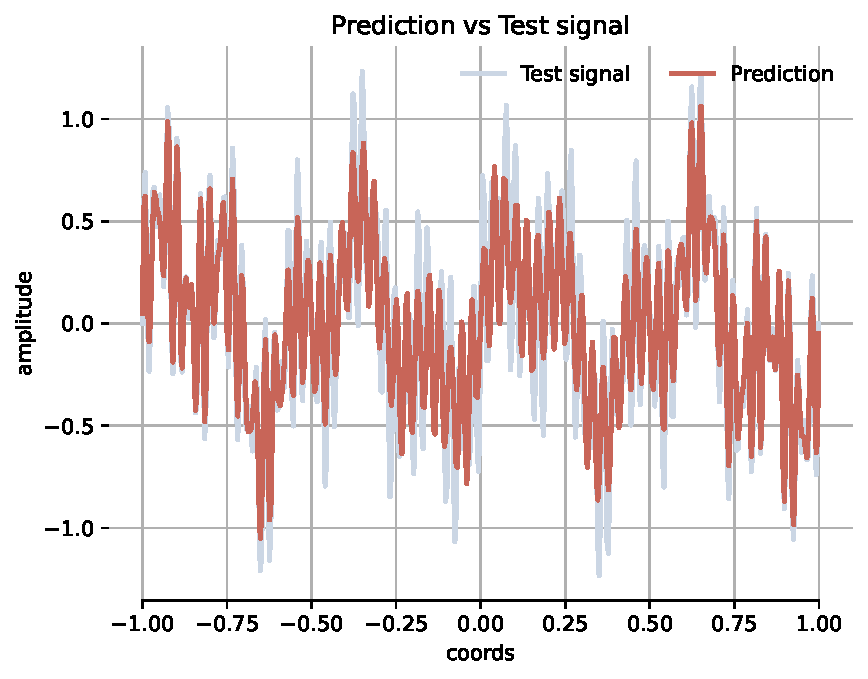
\includegraphics[width=\textwidth]{img/ch3/prediction_w45all_hf128.pdf}
        \caption{128 neurons}
        \label{fig:rec-128-full-45}
    \end{subfigure}
    \begin{subfigure}[b]{0.32\textwidth}
        \centering
        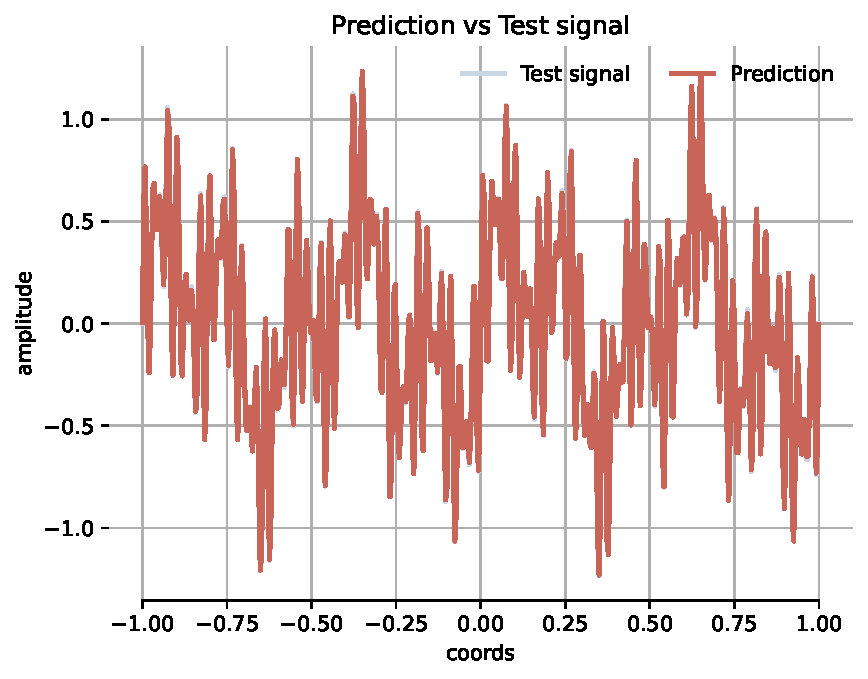
\includegraphics[width=\textwidth]{img/ch3/prediction_w45all_hf256.pdf}
        \caption{256 neurons}
        \label{fig:rec-256-full-45}
    \end{subfigure}
    \begin{subfigure}[b]{0.32\textwidth}
        \centering
        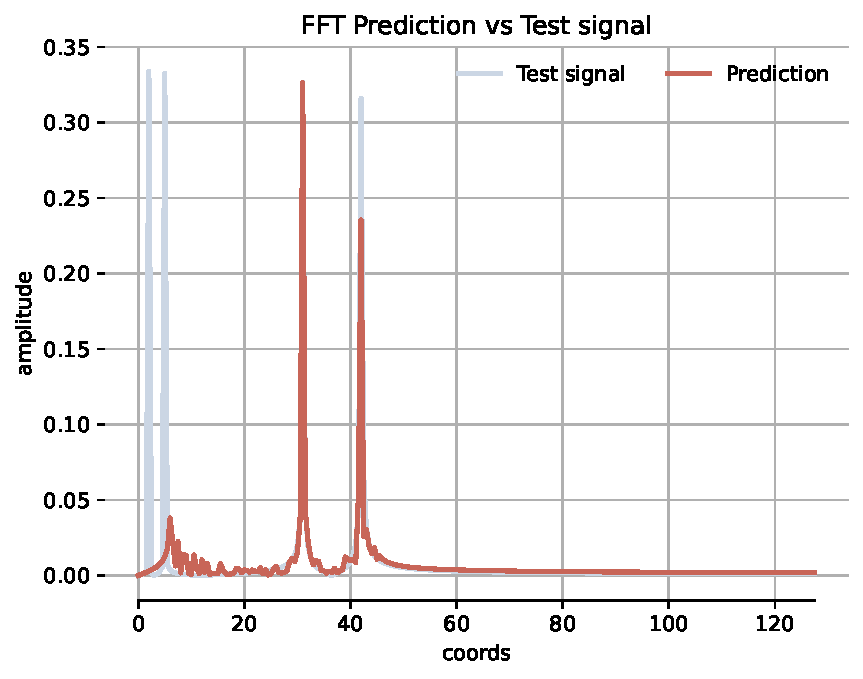
\includegraphics[width=\textwidth]{img/ch3/fft_w45all_hf64.pdf}
        \caption{64 neurons}
        \label{fig:fft-64-full-45}
    \end{subfigure}
    \hfill
    \begin{subfigure}[b]{0.32\textwidth}
        \centering
        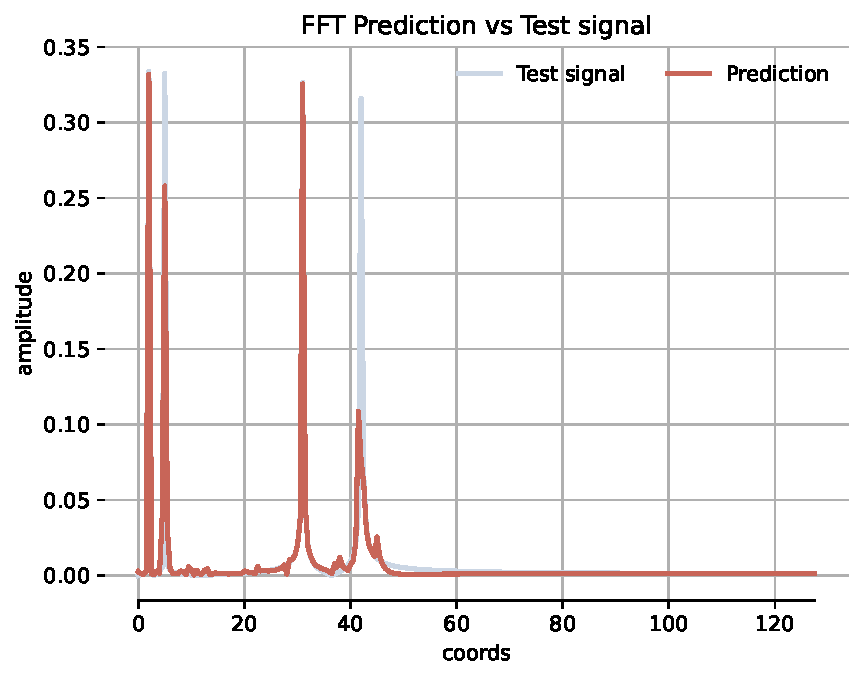
\includegraphics[width=\textwidth]{img/ch3/fft_w45all_hf128.pdf}
        \caption{128 neurons}
        \label{fig:fft-128-full-45}
    \end{subfigure}
    \begin{subfigure}[b]{0.32\textwidth}
        \centering
        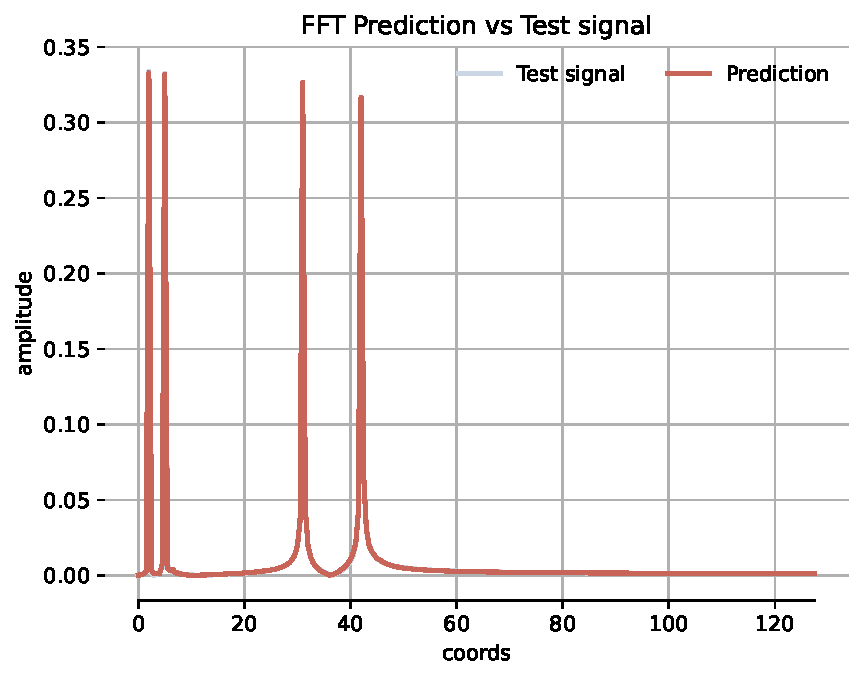
\includegraphics[width=\textwidth]{img/ch3/fft_w45all_hf256.pdf}
        \caption{256 neurons}
        \label{fig:fft-256-full-45}
    \end{subfigure}
    \label{fig:all-freqs-reconstruction}
    \caption{Reconstruction of the signal using networks with different width, all initialized with frequencies in $[-45, 45]$ Hz.}
\end{figure}


These experiments validate our hypothesis that a shallow network with only one layer of sinusoidal activation functions can filter a signal by band-limiting its frequency content, providing a spectral filter similar to those in MFN-based architectures. However, when we add a hidden sinusoidal layer to the network, it becomes much more challenging to isolate specific frequencies. 

Figure \ref{f:w10-1hl-64hf} shows the reconstruction of a sinusoidal network with one hidden layer and 64 neurons per layer, initialized with $\omega_0=10$ Hz. Similar to the experiment with a shallow network of 256 neurons, which was initialized with a broader spectrum of frequencies, the reconstruction seems to perfectly fit the input signal in both the spatial and spectral domains. Figures \ref{fig:4x-freqs-1hl-64hf} and \ref{fig:8x-freqs-1hl-64hf} present two zoomed-in views for a more detailed analysis. In this visualization, the network is evaluated in a grid with 512 samples within a much smaller interval, so most samples were not part of the training data. Notice that the reconstruction is smooth, presenting no spurious noise between the supervised samples.


\begin{figure}[h]
    \centering
    \begin{subfigure}[b]{0.4\textwidth}
        \centering
        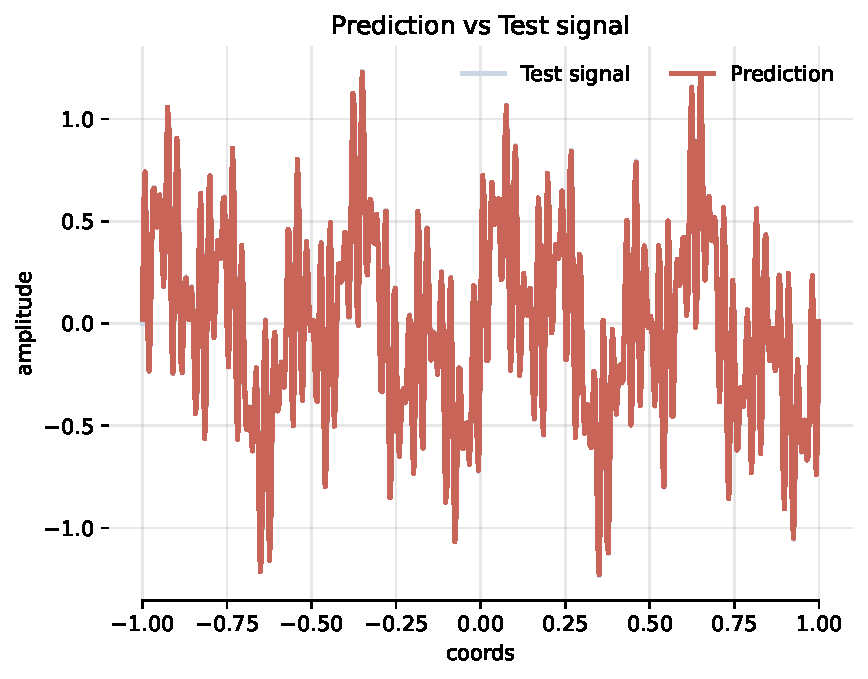
\includegraphics[width=\textwidth]{img/ch3/prediction_1hl_64hf_w10.pdf}
        \caption{Reconstruction}
        \label{fig:rec-freqs-1hl}
    \end{subfigure}
    % \hfill
    \begin{subfigure}[b]{0.4\textwidth}
        \centering
        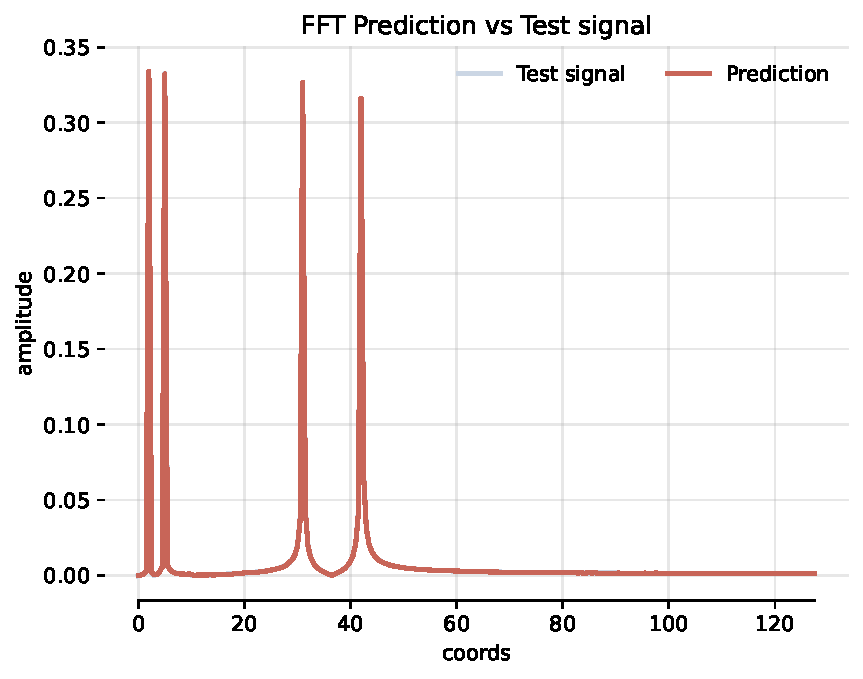
\includegraphics[width=\textwidth]{img/ch3/fft_1hl_64hf_w10.pdf}
        \caption{Frequencies}
        \label{fig:fft-freqs-1hl}
    \end{subfigure}
    
    \begin{subfigure}[b]{0.4\textwidth}
        \centering
        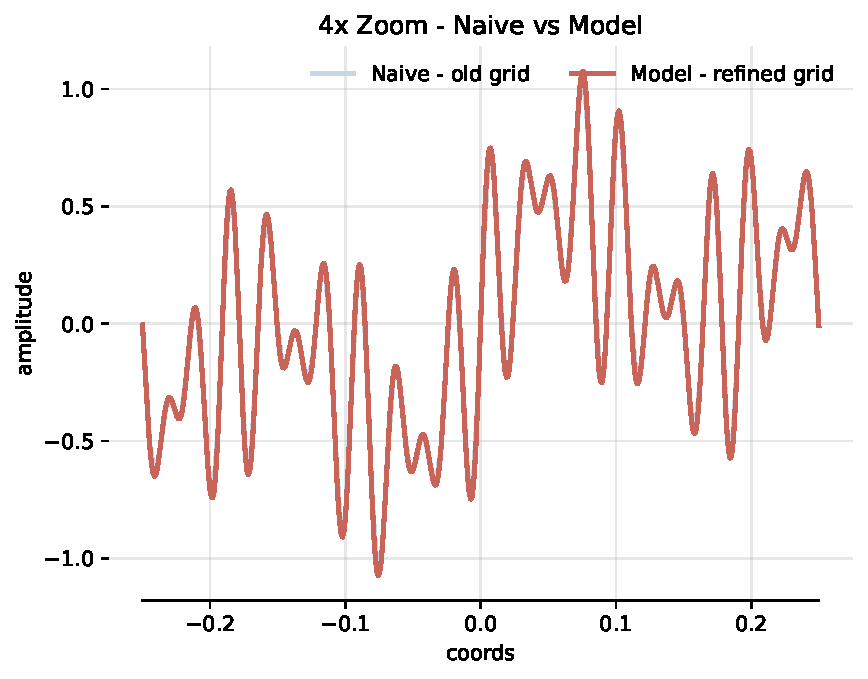
\includegraphics[width=\textwidth]{img/ch3/4x_zoom_1hl_64hf_w10.pdf}
        \caption{Zoom 4x}
        \label{fig:4x-freqs-1hl-64hf}
    \end{subfigure}
    % \hfill
    \begin{subfigure}[b]{0.4\textwidth}
        \centering
        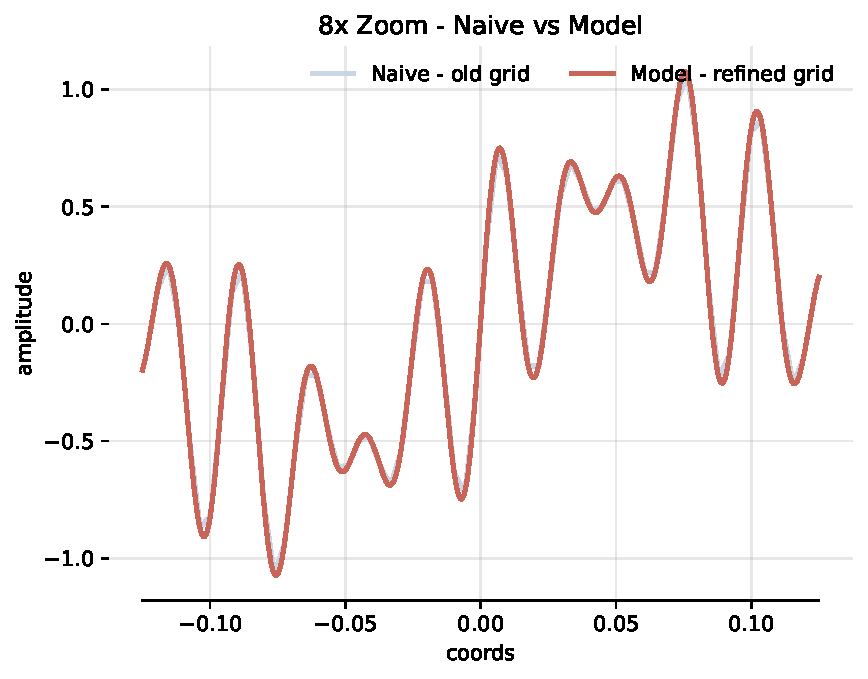
\includegraphics[width=\textwidth]{img/ch3/8x_zoom_1hl_64hf_w10.pdf}
        \caption{Zoom 8x}
        \label{fig:8x-freqs-1hl-64hf}
    \end{subfigure}
    \caption{Reconstruction using 1 hidden layer and 64 neurons per layer.}
    \label{f:w10-1hl-64hf}
\end{figure}

Although the width of the network was kept constant at 64 neurons, adding a single hidden layer significantly increases the size of the model, and thus its capacity, which could explain why it fits the signal better, even though it was initialized with lower frequencies. For instance, a shallow model with 64 neurons per layer has $192$ parameters, while a model with 1 hidden layer and 64 neurons per layer has $4352$ parameters.

To better understand the impact of the hidden layer, we conducted additional experiments, reducing the width of the networks with 1 hidden layer and increasing the width of those without hidden layers. For these experiments, all models were initialized with frequencies in the range $[-10, 10]$ Hz. Figure \ref{fig:rec-1hl-16hf-w10} shows the reconstruction of a model with 1 hidden layer and 16 neurons per layer, with a total of $320$ parameters. Note that this model still captures the high frequencies in the signal, although some noise is visible in its FFT (Figure \ref{fig:fft-1hl-16hf-w10}). However, the model with no hidden layers and 1024 neurons per layer is unable to capture any of the high frequencies (Figures \ref{fig:rec-0hl-1024-w10hf} and \ref{fig:fft-0hl-1024-w10hf}), despite having $3072$ parameters. We conclude that the hidden layer, rather than the model size, is primarily responsible for this behavior.

\begin{figure}[h!]
    \centering
    \begin{subfigure}[b]{0.40\textwidth}
        \centering
        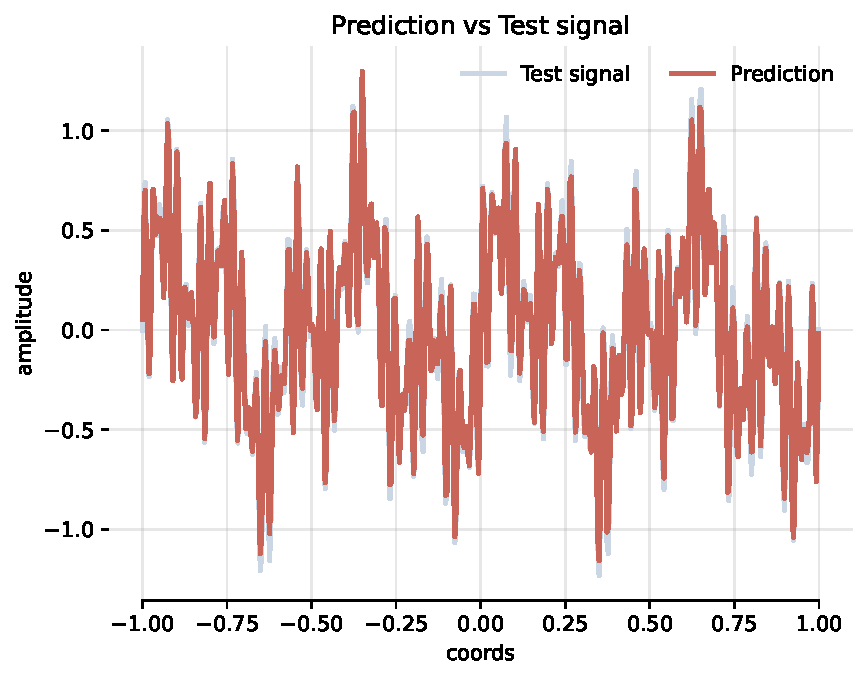
\includegraphics[width=\textwidth]{img/ch3/prediction_1hl_16hf_w10.pdf}
        \caption{1 hidden layer, 16 neurons}
        \label{fig:rec-1hl-16hf-w10}
    \end{subfigure}
    % \hfill
    \begin{subfigure}[b]{0.40\textwidth}
        \centering
        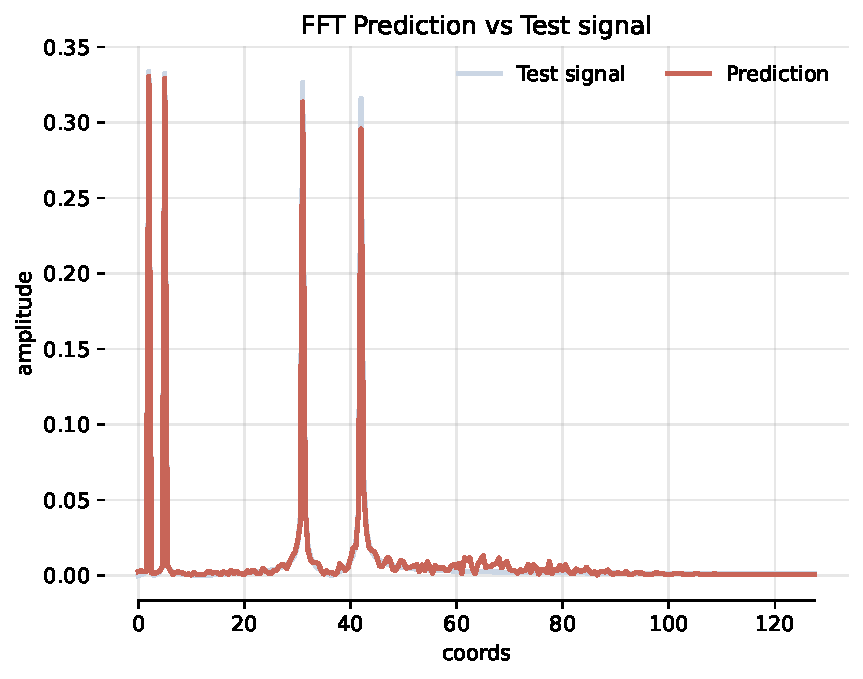
\includegraphics[width=\textwidth]{img/ch3/fft_1hl_16hf_w10.pdf}
        \caption{1 hidden layer, 16 neurons}
        \label{fig:fft-1hl-16hf-w10}
    \end{subfigure}
    
    \begin{subfigure}[b]{0.40\textwidth}
        \centering
        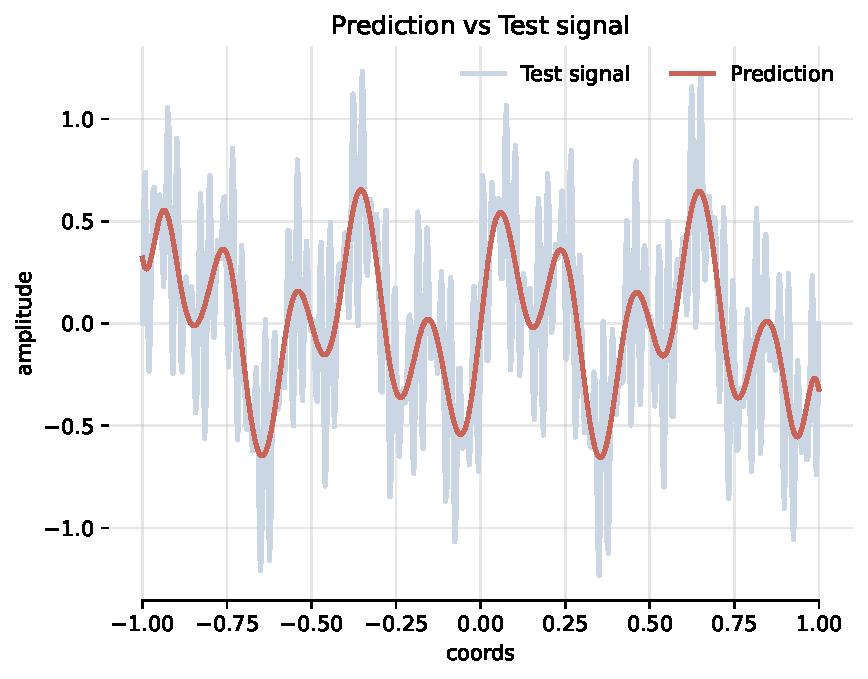
\includegraphics[width=\textwidth]{img/ch3/prediction_0hl_1024hf_w10.pdf}
        \caption{No hidden layers}
        \label{fig:rec-0hl-1024-w10hf}
    \end{subfigure}
    % \hfill
    \begin{subfigure}[b]{0.40\textwidth}
        \centering
        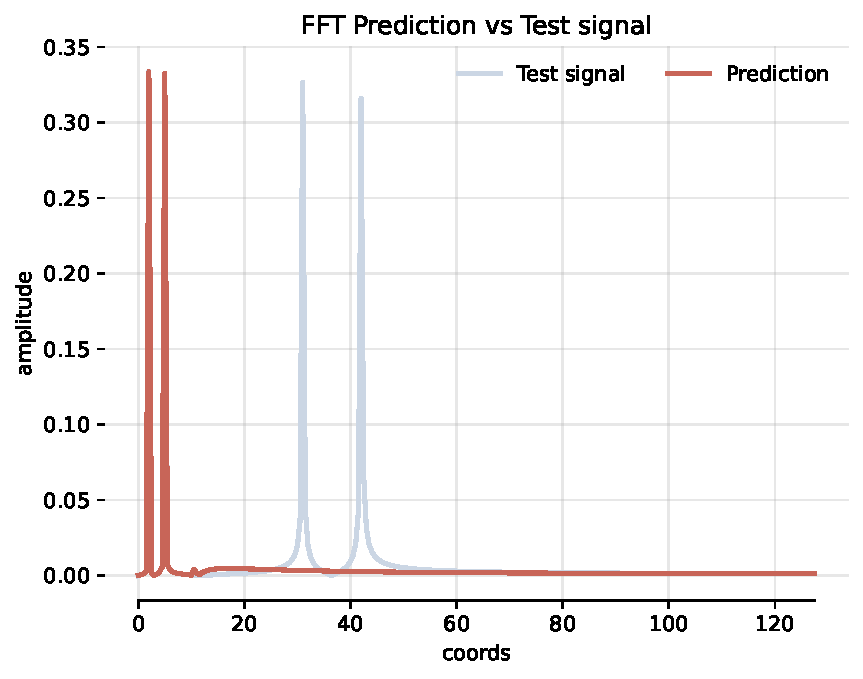
\includegraphics[width=\textwidth]{img/ch3/fft_0hl_1024hf_w10.pdf}
        \caption{No hidden layers}
        \label{fig:fft-0hl-1024-w10hf}
    \end{subfigure}
    \caption{Comparison of a smaller model with a single hidden layer to a larger model without hidden layers.}
    \label{f:hidden-layer-vs-no-hiddel-layer}
\end{figure}

We ran new experiments using frequencies in the range $[-35, -25] \cup [25, 35]$ (hertz) to initilize the networks and observed a similar phenomenon in the highest frequencies. Figure \ref{fig:rec-1hl-16hf-35w45} shows that a network with 1 hidden layer and 16 neurons per layer can capture the lower frequencies, despite showing some noise in its spectrum (Figure \ref{fig:fft-1hl-16hf-35w45}), while a network with no hidden layers and 1024 neurons per layer fails to capture the lower frequencies (Figures \ref{fig:rec-1hl-1024hf-35w45} and \ref{fig:fft-1hl-1024hf-35w45}).

\begin{figure}[h!]
    \centering
    \begin{subfigure}[b]{0.40\textwidth}
        \centering
        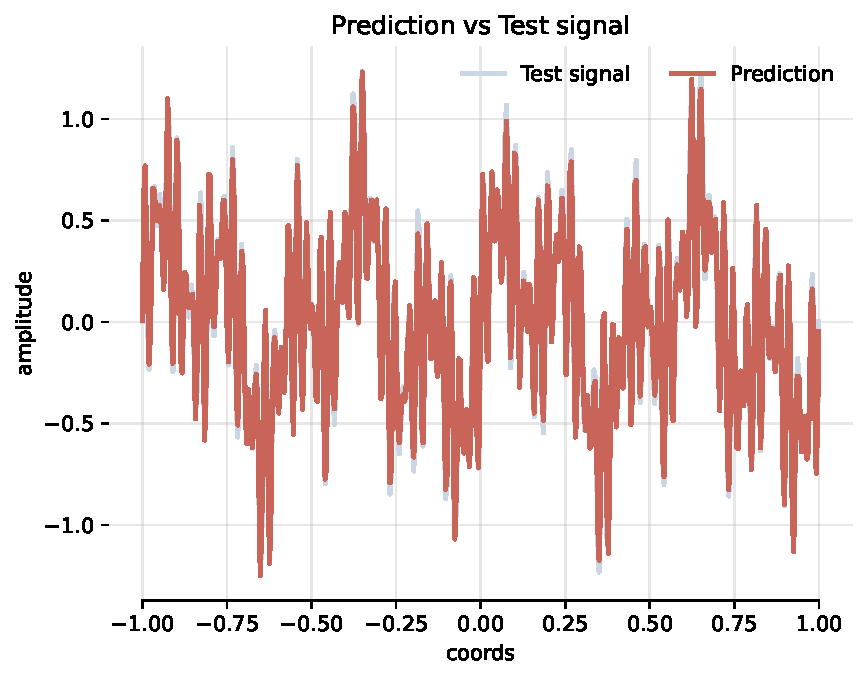
\includegraphics[width=\textwidth]{img/ch3/prediction_1hl_16hf_35w45.pdf}
        \caption{1 hidden layer, 16 neurons}
        \label{fig:rec-1hl-16hf-35w45}
    \end{subfigure}
    % \hfill
    \begin{subfigure}[b]{0.40\textwidth}
        \centering
        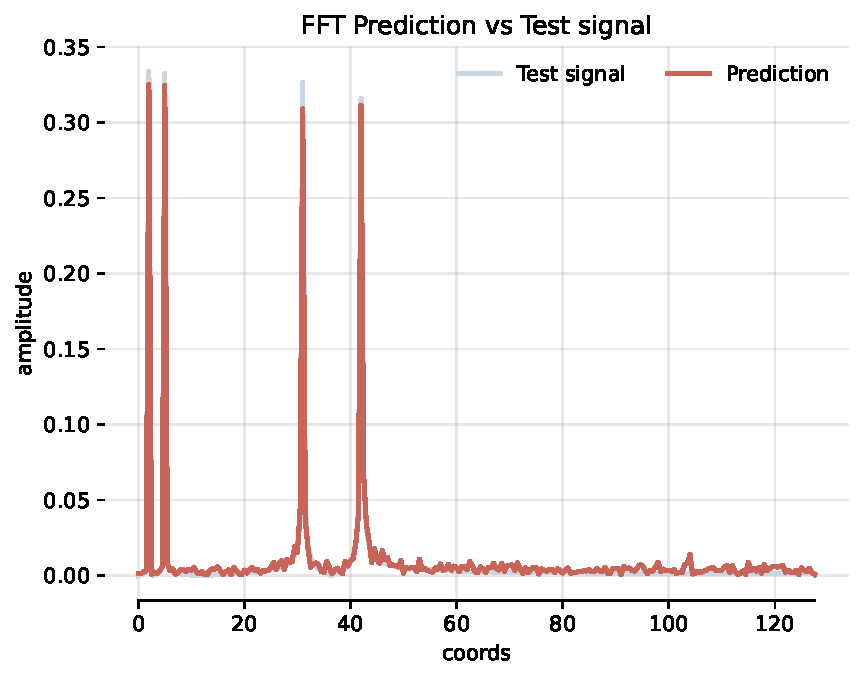
\includegraphics[width=\textwidth]{img/ch3/fft_1hl_16hf_35w45.pdf}
        \caption{1 hidden layer, 16 neurons}
        \label{fig:fft-1hl-16hf-35w45}
    \end{subfigure}
    
    \begin{subfigure}[b]{0.40\textwidth}
        \centering
        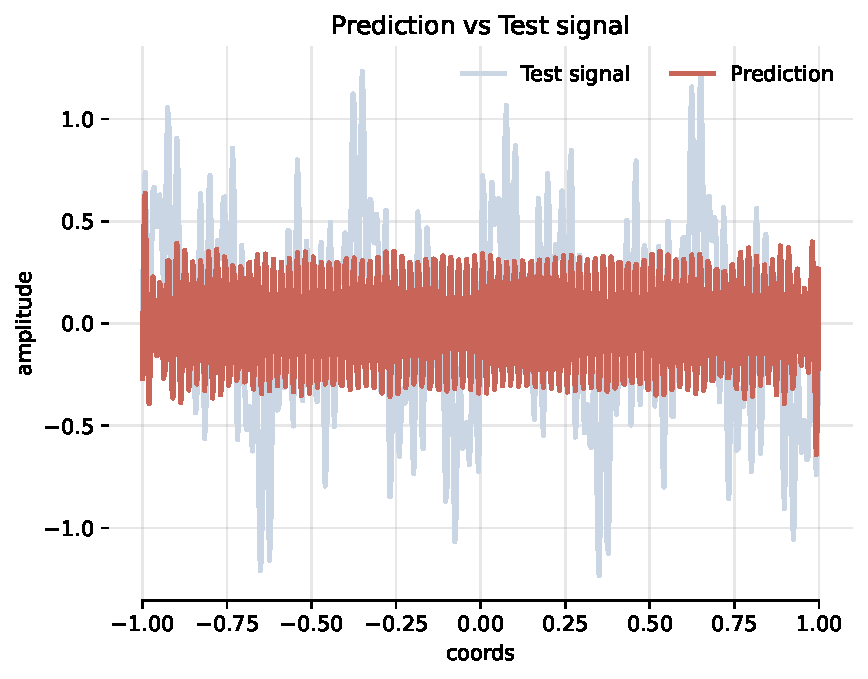
\includegraphics[width=\textwidth]{img/ch3/prediction_1hl_1024hf_35w45.pdf}
        \caption{No hidden layers}
        \label{fig:rec-1hl-1024hf-35w45}
    \end{subfigure}
    % \hfill
    \begin{subfigure}[b]{0.40\textwidth}
        \centering
        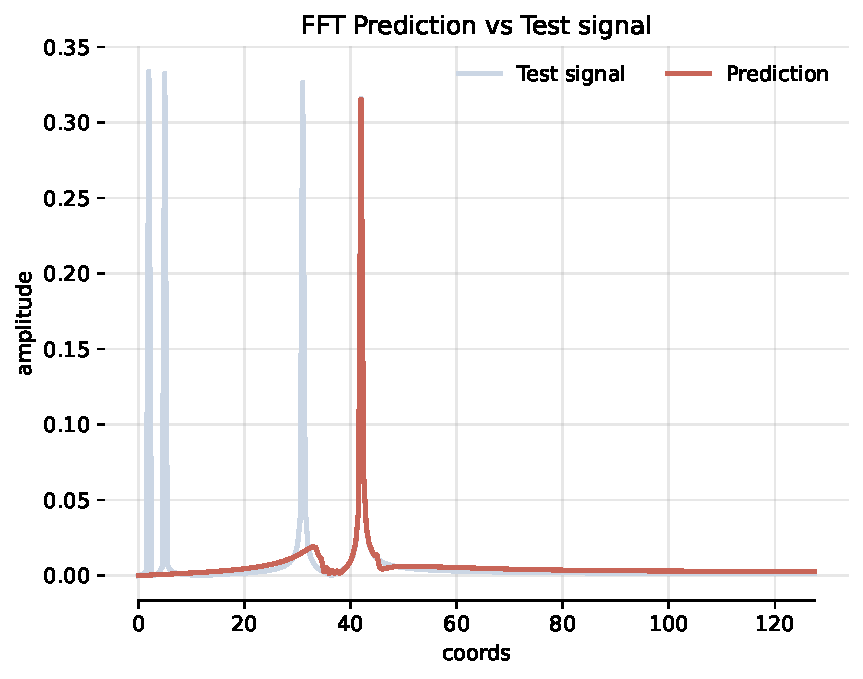
\includegraphics[width=\textwidth]{img/ch3/fft_1hl_1024hf_35w45.pdf}
        \caption{No hidden layers}
        \label{fig:fft-1hl-1024hf-35w45}
    \end{subfigure}
    \caption{Comparison between smaller model with 1 hidden layer and bigger model without hidden layer when models are initialized only with high frequencies.}
    \label{f:hiddenlayer-vs-nohl-high-frequencies}
\end{figure}


We conclude that a sinusoidal neural network with no hidden layers can effectivelly filter and decompose the frequencies of a sinal. However, in general, it not straightforward to decompose the frequencies of a signal using a sinusoidal deep network with at least one hidden layer.

\pagebreak

\subsection{Learning and filtering stochastic signals}

%     - Diverging by using high frequencies. Show how the network diverges when initialized with very high frequencies.


After experimenting with signals containing a few controlled frequencies, we procedurally generated stochastic signals using a technique known as Perlin Noise (\cite{perlin-1985}). This approach allows us to analyze how a sinusoidal model learns a distribution of frequencies across a broad range. For the following experiments, we sampled 2048 points uniformly from the interval $[-1, 1]$, yielding a sampling rate of 1/1024. According to the Shannon-Nyquist sampling theorem, this limits us to frequencies up to 512 Hz. The parameters for generating the Perlin Noise signal were: scale = 10; octaves = 16; persistence = 1.4.

We began by training a shallow sinusoidal network as a sanity check. The expectation was for the network to capture only the lowest frequencies, up to the range determined by its initialization parameter, $\omega_0$. We used a network with 512 hidden neurons per layer, varying the value of $\omega_0$. Figure \ref{f:rec-noise-shallow} shows the reconstruction in both spatial and frequency domains for $\omega_0 \in \{8, 64, 128\}$ Hz. Note that the FFT plot displays a distribution of frequencies up to 512 Hz, with higher amplitudes for the lower frequencies. As expected, the results resemble smoothed versions of the signal, as the network captures only the frequencies up to the value of $\omega_0$.

\begin{figure}[h]
    \centering
    \begin{subfigure}[b]{0.32\textwidth}
        \centering
        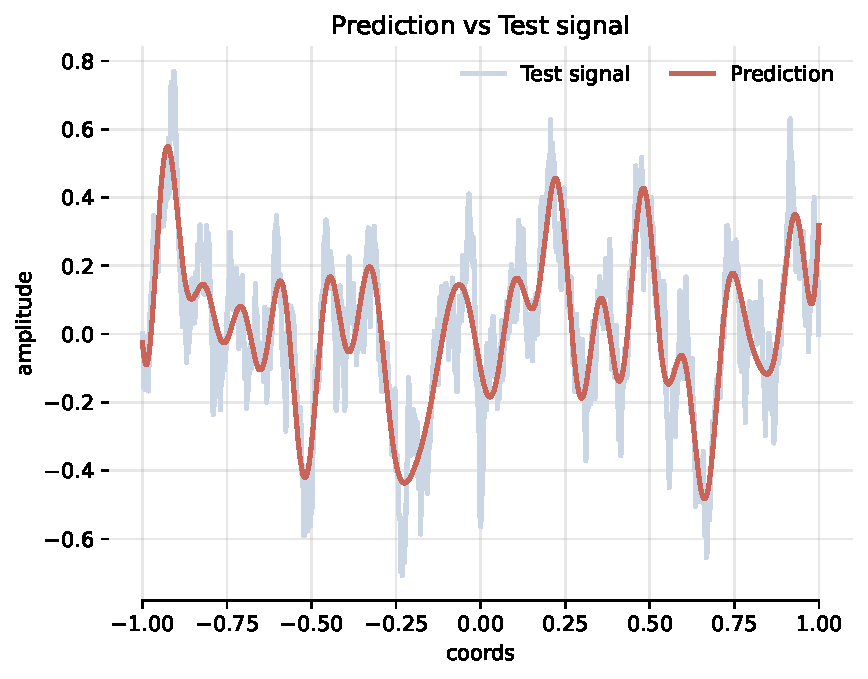
\includegraphics[width=\textwidth]{img/ch3/pred-noise-h0-w8.pdf}
        \caption{$\omega_0=8$}
        \label{fig:rec-noise-shallow-w8}
    \end{subfigure}
    \hfill
    \begin{subfigure}[b]{0.32\textwidth}
        \centering
        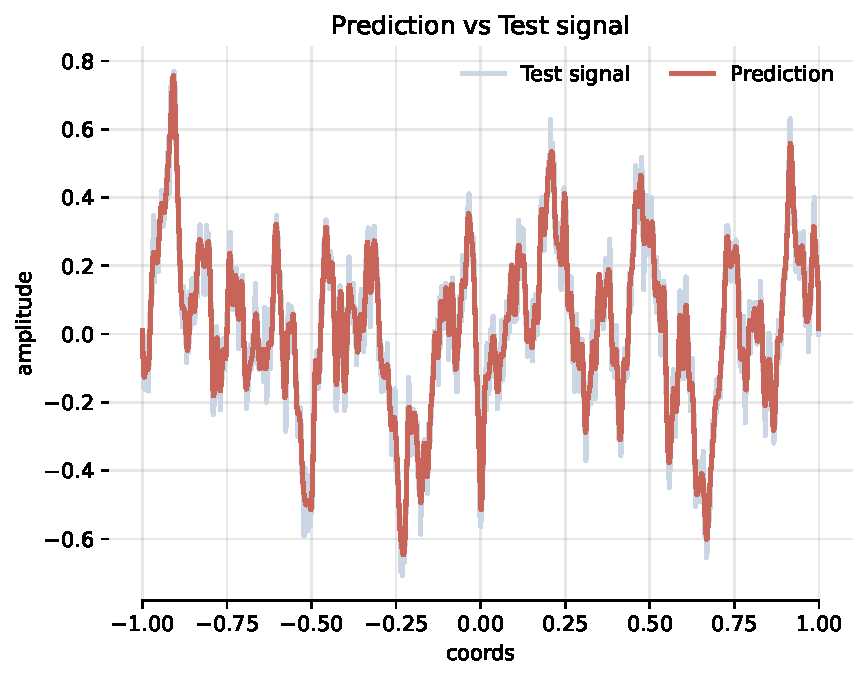
\includegraphics[width=\textwidth]{img/ch3/pred-noise-h0-w64.pdf}
        \caption{$\omega_0=64$}
        \label{fig:rec-noise-shallow-w64}
    \end{subfigure}
    \hfill
    \begin{subfigure}[b]{0.32\textwidth}
        \centering
        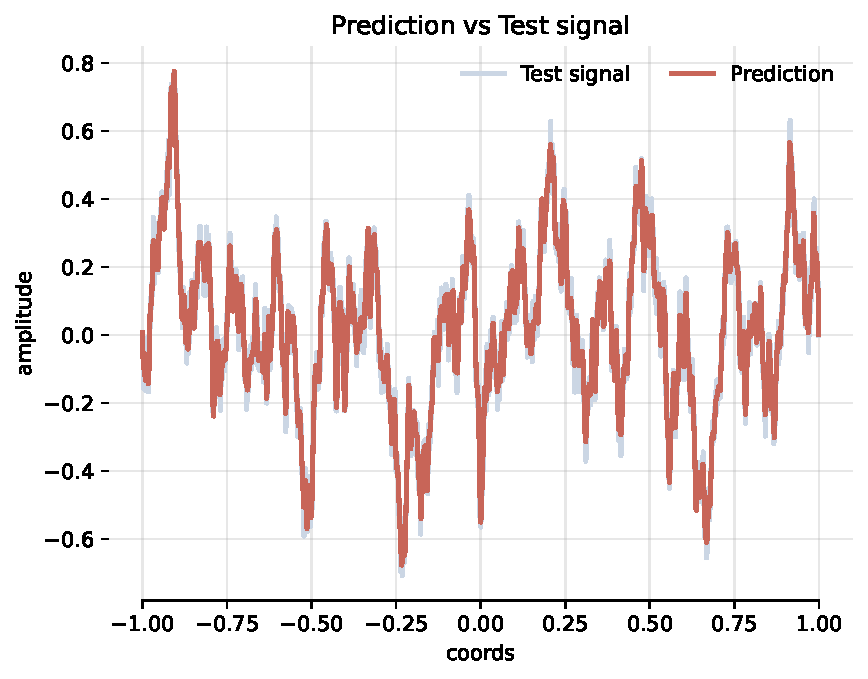
\includegraphics[width=\textwidth]{img/ch3/pred-noise-h0-w128.pdf}
        \caption{$\omega_0=128$}
        \label{fig:rec-noise-shallow-w128}
    \end{subfigure}

    \begin{subfigure}[b]{0.32\textwidth}
        \centering
        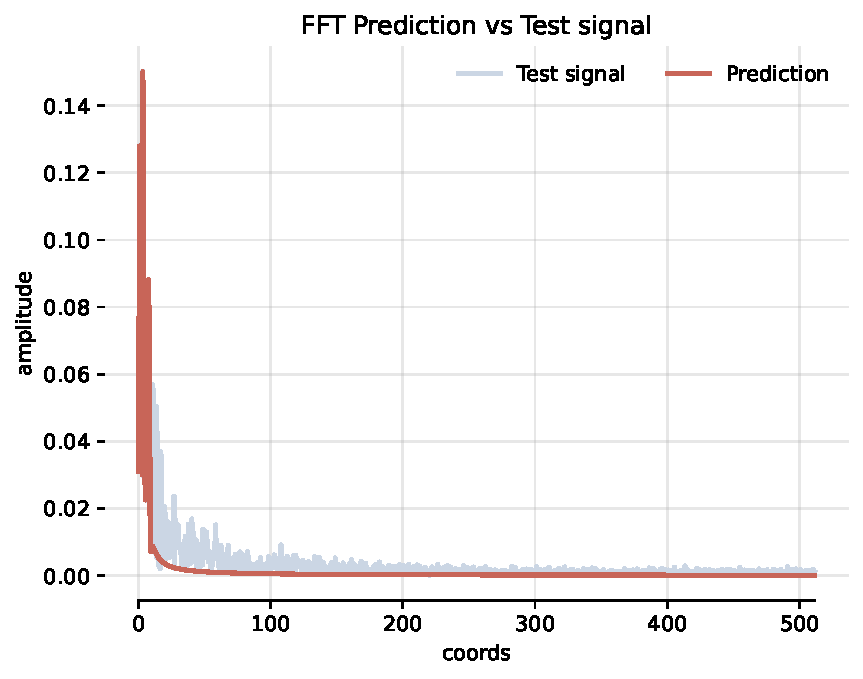
\includegraphics[width=\textwidth]{img/ch3/fft-noise-h0-w8.pdf}
        \caption{$\omega_0=8$}
        \label{fig:fft-noise-shallow-w8}
    \end{subfigure}
    \hfill
    \begin{subfigure}[b]{0.32\textwidth}
        \centering
        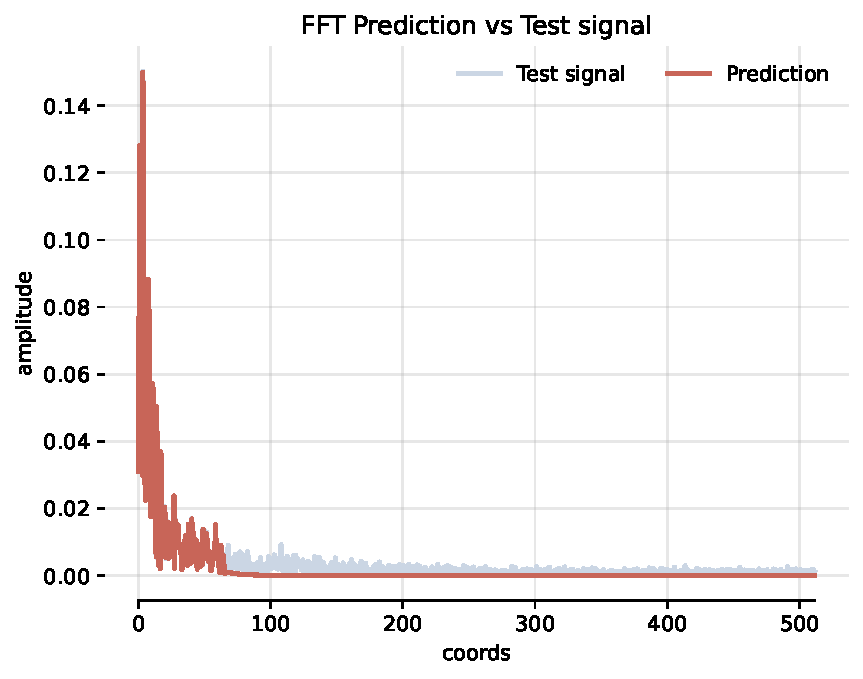
\includegraphics[width=\textwidth]{img/ch3/fft-noise-h0-w64.pdf}
        \caption{$\omega_0=64$}
        \label{fig:fft-noise-shallow-w64}
    \end{subfigure}
    \hfill
    \begin{subfigure}[b]{0.32\textwidth}
        \centering
        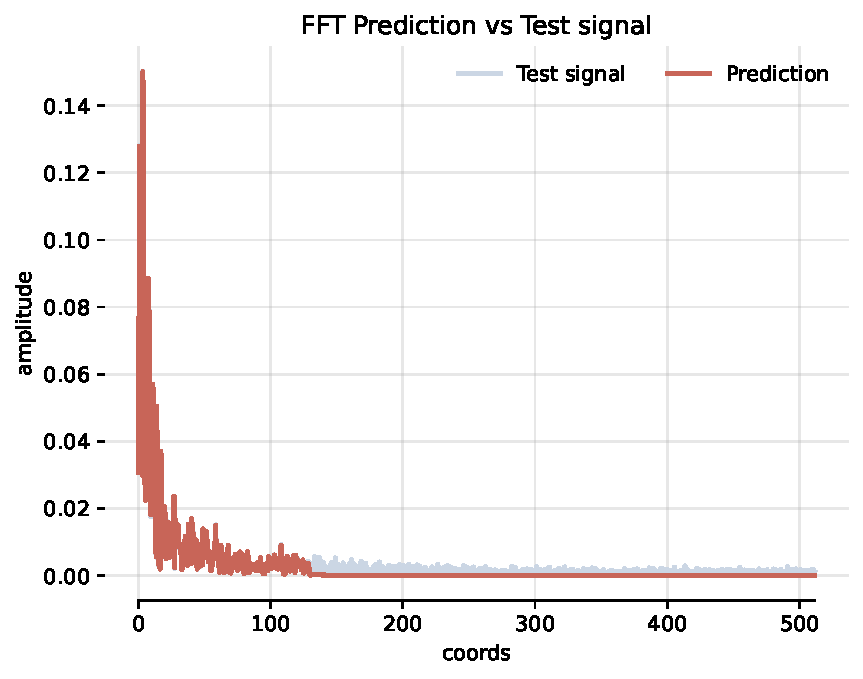
\includegraphics[width=\textwidth]{img/ch3/fft-noise-h0-w128.pdf}
        \caption{$\omega_0=128$}
        \label{fig:fft-noise-shallow-w128}
    \end{subfigure}
    \caption{Reconstruction of a stochastic signal using shallow sinusoidal networks initilized with different frequency ranges.}
    \label{f:rec-noise-shallow}
\end{figure}

As we increase $\omega_0$ to capture higher frequencies, we observe a phenomenon similar to that seen in Figure \ref{fig:fft-64-full-45}: the model's performance deteriorates for some of the lower frequencies, and noise is introduced due to insufficient capacity. This situation is illustrated in Figure \ref{f:rec-noise-shallow-hf512-w256}.

\begin{figure}[h]
    \centering
    \begin{subfigure}[b]{0.40\textwidth}
        \centering
        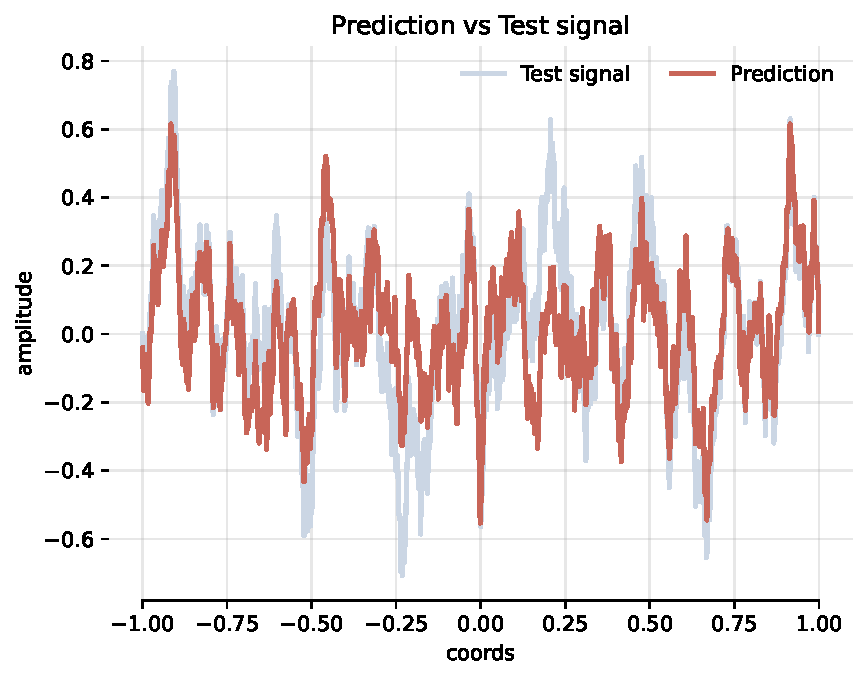
\includegraphics[width=\textwidth]{img/ch3/pred-noise-h0-hf512-w256.pdf}
        \caption{}
    \end{subfigure}
    % \hfill
    \begin{subfigure}[b]{0.40\textwidth}
        \centering
        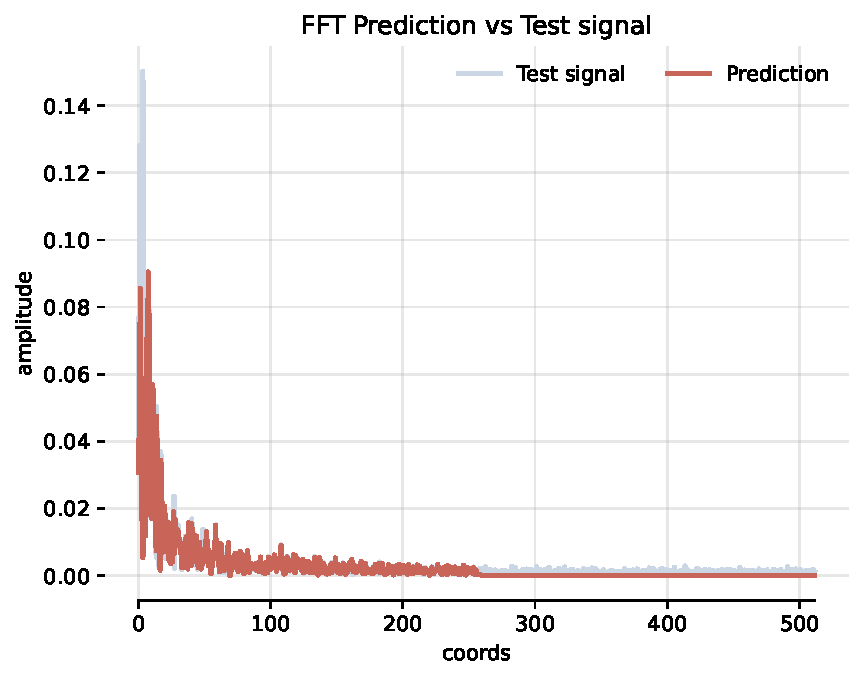
\includegraphics[width=\textwidth]{img/ch3/fft-noise-h0-hf512-w256.pdf}
        \caption{}
        % \label{fig:fft-noise-shallow-hf512-w256}
    \end{subfigure}
    \caption{Reconstruction of signal (A) and frequencies (B) using 512 neurons per layer and $\omega_0=256$}
    \label{f:rec-noise-shallow-hf512-w256}
\end{figure}

We also noticed significant oscillations in the loss function curve in experiments involving larger frequencies. Figure \ref{f:loss-noise-comparison-hl0-hf512} presents the mean squared error per epoch during the training of networks with $\omega_0=64$ and $\omega_0=256$. Based on these observations, we reduced the learning rate to 0.0001, increased the number of training epochs to 400, and ran new experiments. Figure \ref{f:full-noise-hf4096-w512} shows the results from these updated experiments, using 4096 neurons per layer, with zoomed-in views for detailed analysis.

\begin{figure}[h]
    \centering
    \begin{subfigure}[b]{0.45\textwidth}
        \centering
        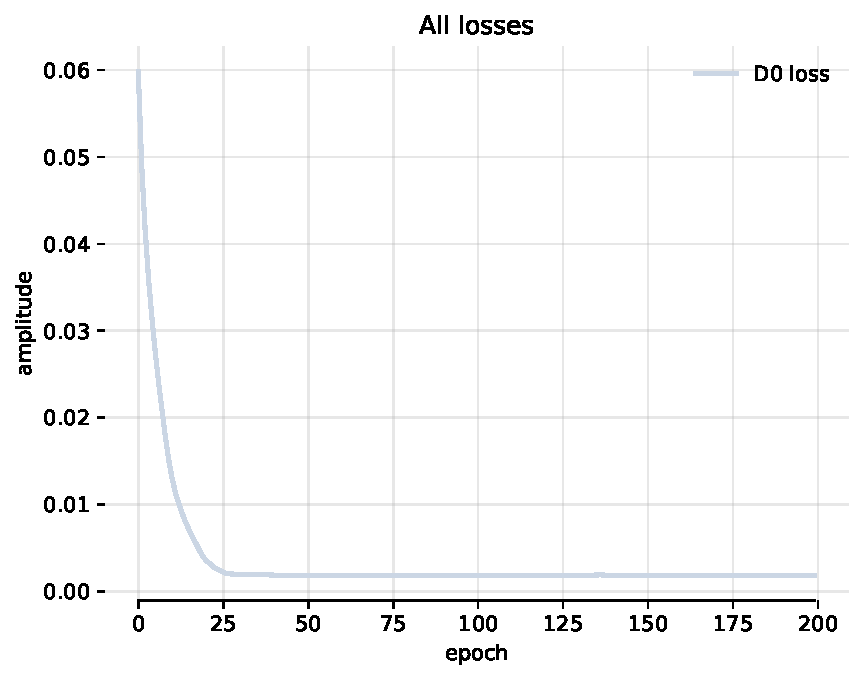
\includegraphics[width=\textwidth]{img/ch3/loss-noise-hl0-hf512-w64.pdf}
        \caption{$\omega_0=64$}
        \label{fig:loss-hf512-w64}
    \end{subfigure}
    \begin{subfigure}[b]{0.45\textwidth}
        \centering
        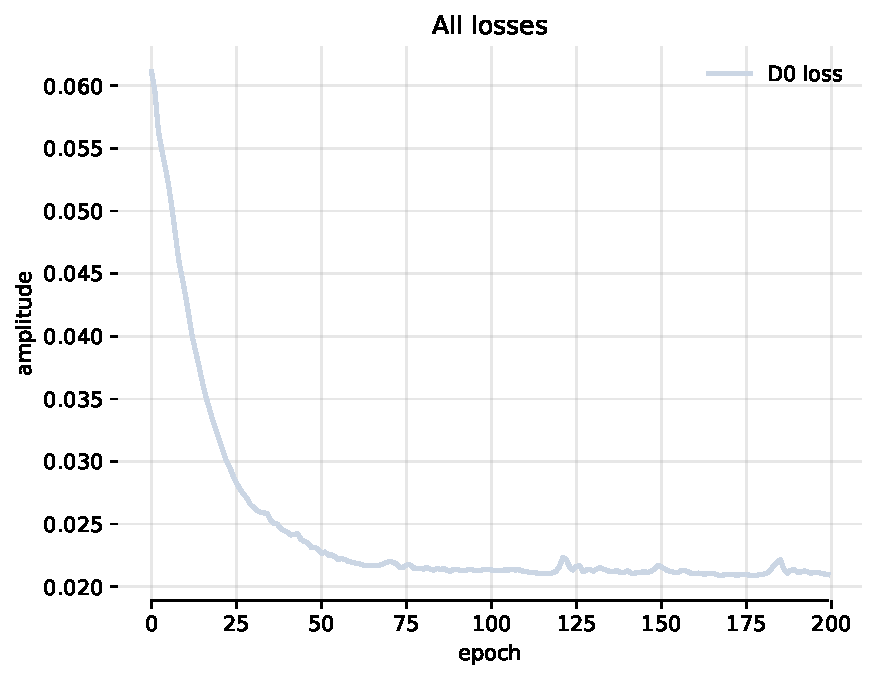
\includegraphics[width=\textwidth]{img/ch3/loss-noise-hl0-hf512-w256.pdf}
        \caption{$\omega_0=256$}
        \label{fig:loss-hf512-w256}
    \end{subfigure}
    \caption{Mean squared error per epoch when training with 512 neurons per layer.}
    \label{f:loss-noise-comparison-hl0-hf512}
\end{figure}


\begin{figure}[h]
    \centering
    \begin{subfigure}[b]{0.32\textwidth}
        \centering
        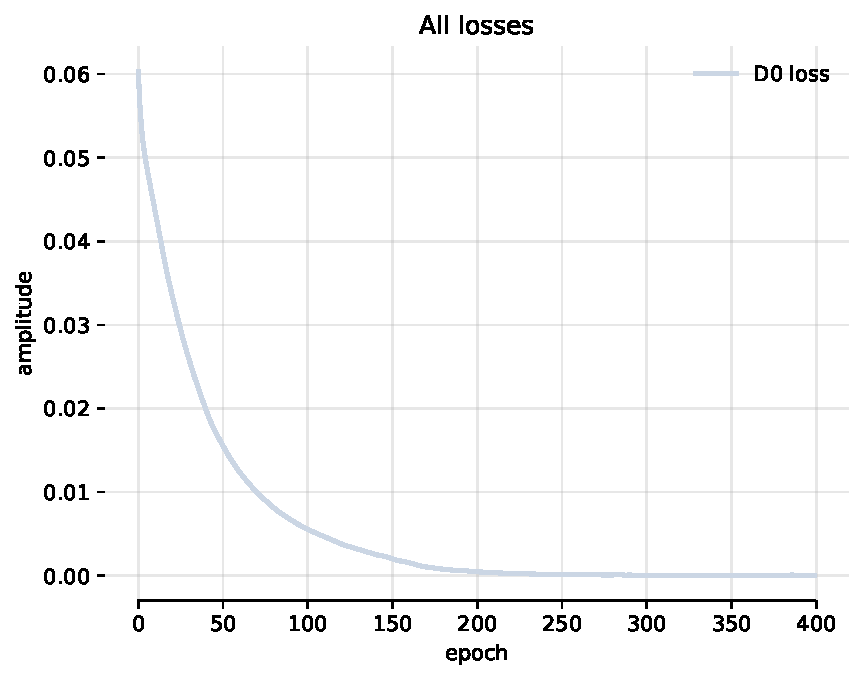
\includegraphics[width=\textwidth]{img/ch3/loss-noise-hf4096-w512.pdf}
        \caption{Loss}
    \end{subfigure}
    \begin{subfigure}[b]{0.32\textwidth}
        \centering
        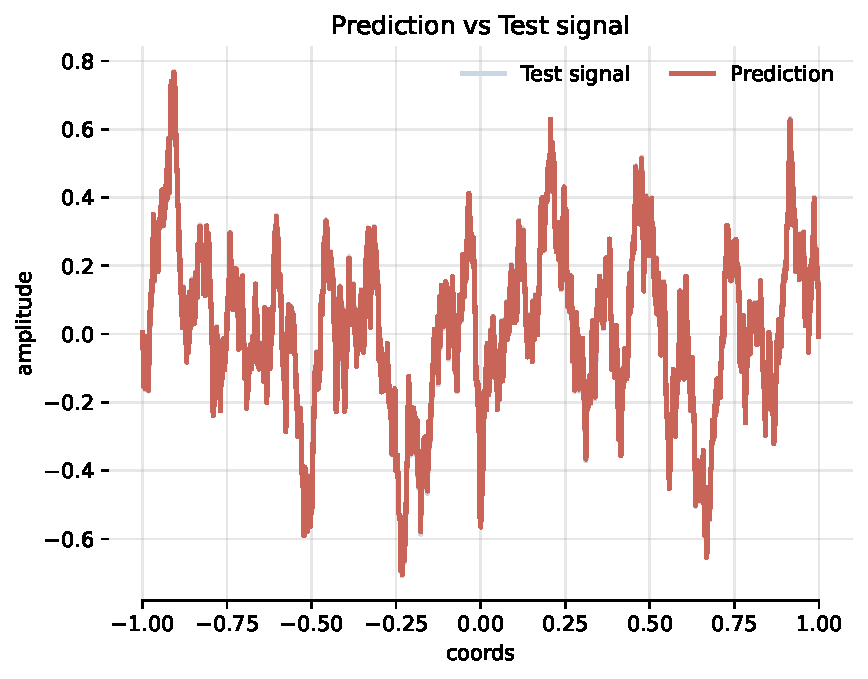
\includegraphics[width=\textwidth]{img/ch3/pred-noise-hf4096-w512.pdf}
        \caption{Reconstruction}
    \end{subfigure}
    \begin{subfigure}[b]{0.32\textwidth}
        \centering
        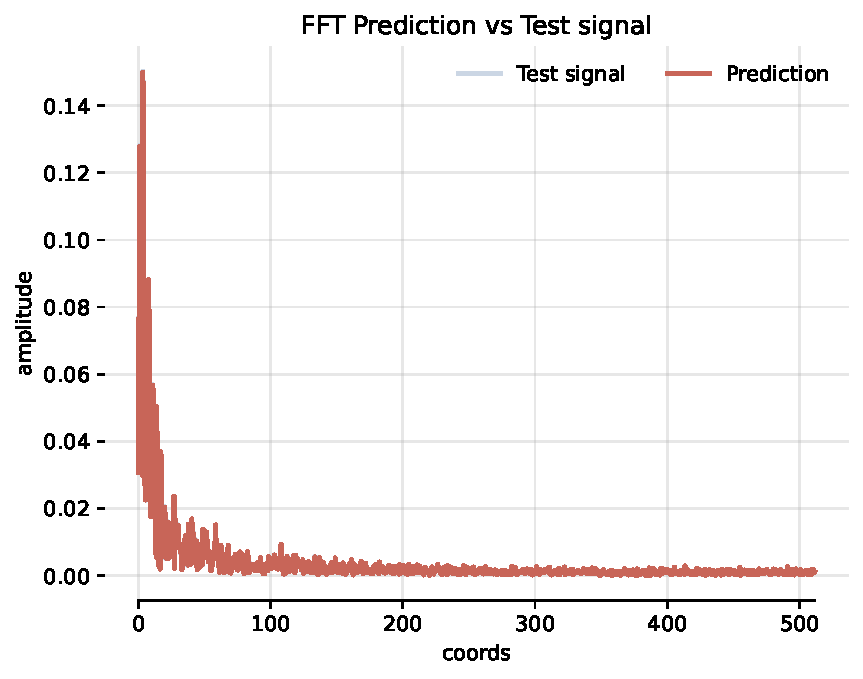
\includegraphics[width=\textwidth]{img/ch3/fft-noise-hf4096-w512.pdf}
        \caption{Frequencies}
    \end{subfigure}

    \begin{subfigure}[b]{0.32\textwidth}
        \centering
        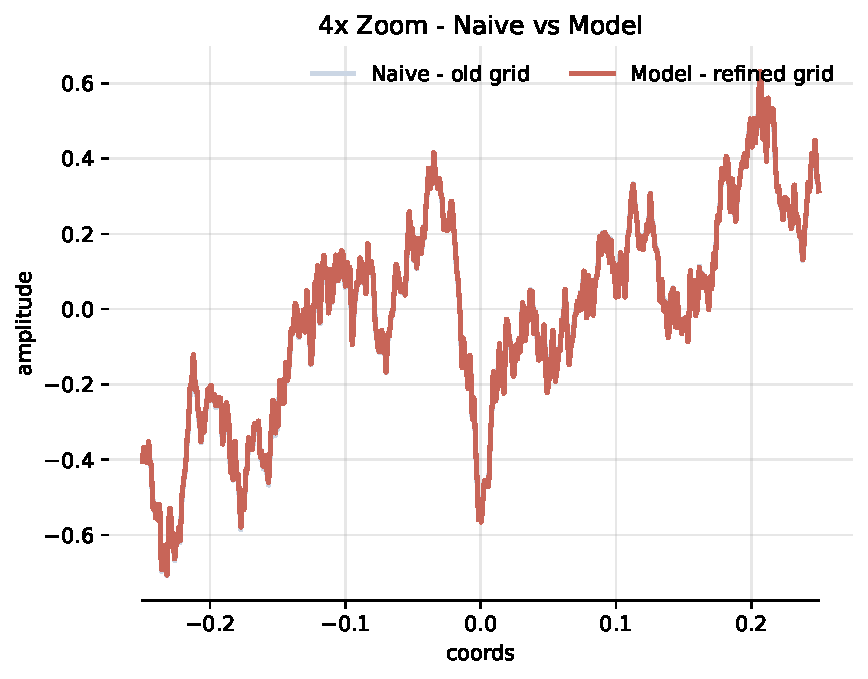
\includegraphics[width=\textwidth]{img/ch3/noise-4x-hf4096-w512.pdf}
        \caption{4x zoom}
    \end{subfigure}
    \begin{subfigure}[b]{0.32\textwidth}
        \centering
        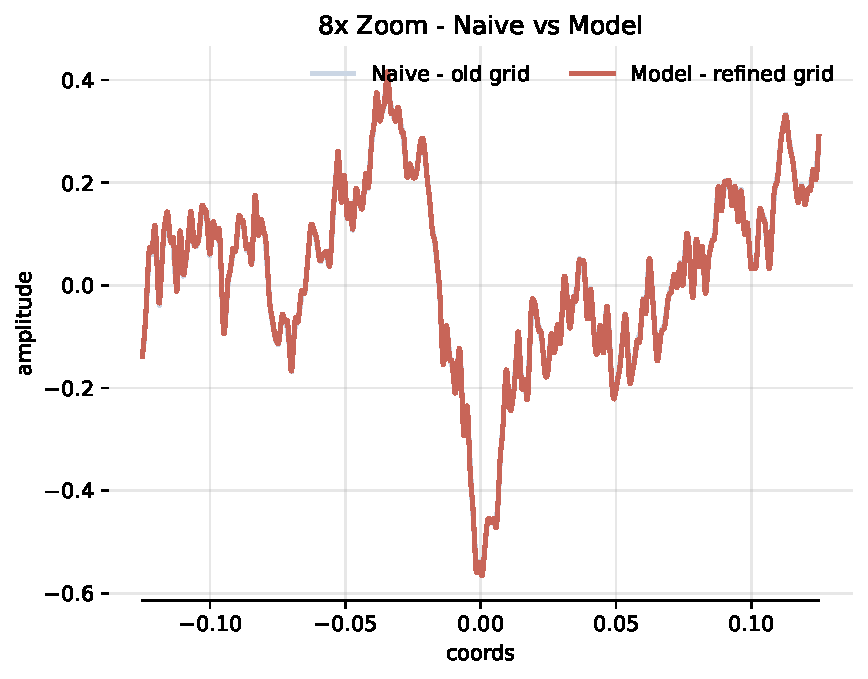
\includegraphics[width=\textwidth]{img/ch3/noise-8x-hf4096-w512.pdf}
        \caption{8x zoom}
    \end{subfigure}
    \begin{subfigure}[b]{0.32\textwidth}
        \centering
        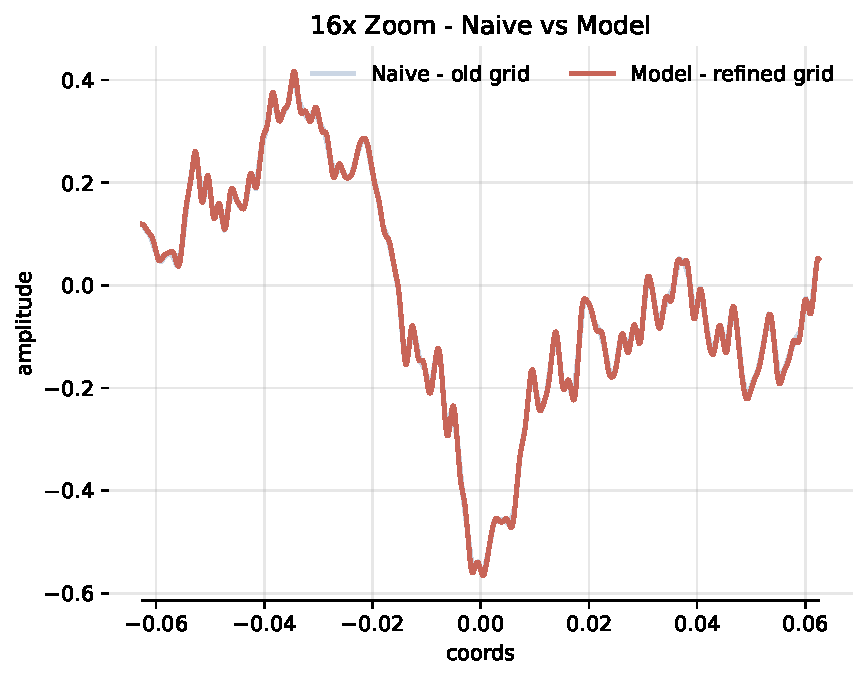
\includegraphics[width=\textwidth]{img/ch3/noise-16x-hf4096-w512.pdf}
        \caption{16x zoom}
    \end{subfigure}
    \caption{Reconstruction results using a shallow network with 4096 neurons per layer and $\omega_0=512$}
    \label{f:full-noise-hf4096-w512}
\end{figure}


In the following experiments, we employed sinusoidal neural networks with one hidden layer. The primary question we wanted to investigate was: \emph{can smaller, but deeper, networks learn bounded frequencies?} The answer is "yes", but it requires careful tuning.

First, it is important to note that introducing a hidden layer greatly increases the network's capacity to generate higher frequencies. Figure \ref{f:rec-1hl-32hf-8hz} shows the reconstruction of the same Perlin noise used in previous experiments, but this time using a network with 1 hidden layer and 32 neurons per layer, initialized with $\omega_0=8$ Hz. As in the initial experiments with shallow networks, the model was trained for 200 epochs with a learning rate of 0.001.

\begin{figure}[h]
    \centering
    \begin{subfigure}[b]{0.32\textwidth}
        \centering
        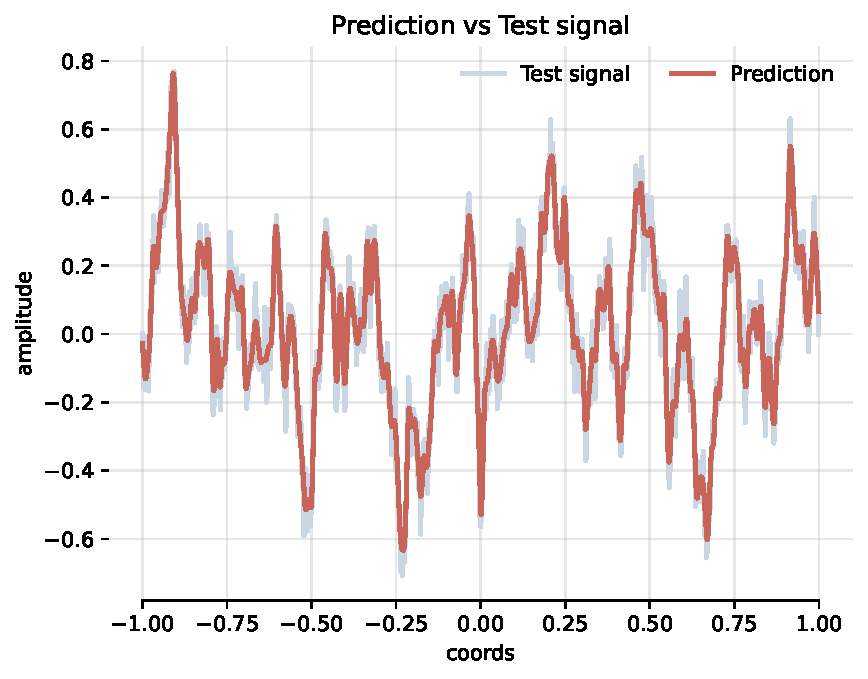
\includegraphics[width=\textwidth]{img/ch3/pred-noise-1hl-32hf-w8.pdf}
        \caption{}
        \label{fig:pred-noise-1hl-32hf-w8}
    \end{subfigure}
    \begin{subfigure}[b]{0.32\textwidth}
        \centering
        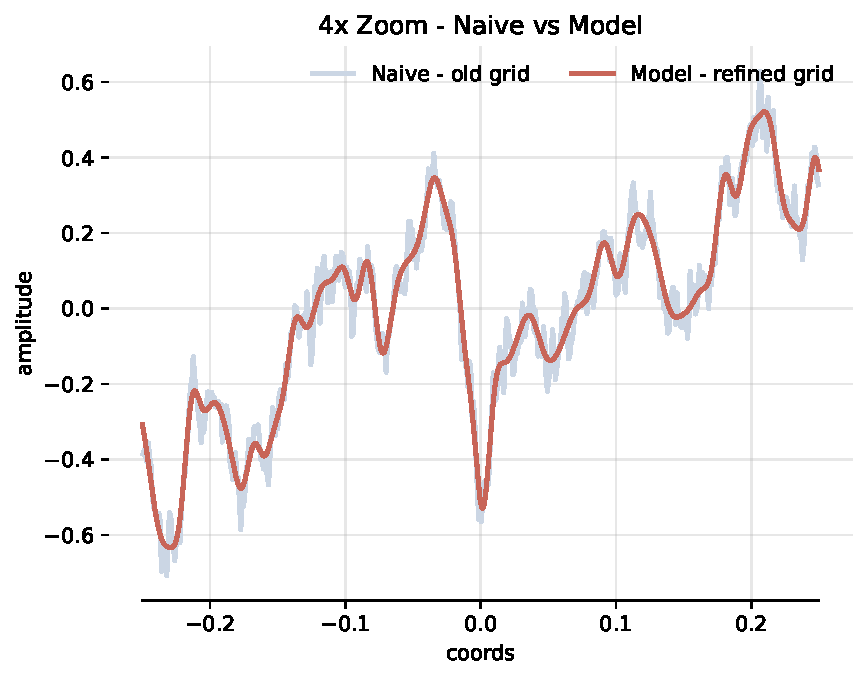
\includegraphics[width=\textwidth]{img/ch3/4x-zoom-noise-1hl-32hf-w8.pdf}
        \caption{}
        \label{fig:4x-zoom-noise-1hl-32hf-w8}
    \end{subfigure}
    \begin{subfigure}[b]{0.32\textwidth}
        \centering
        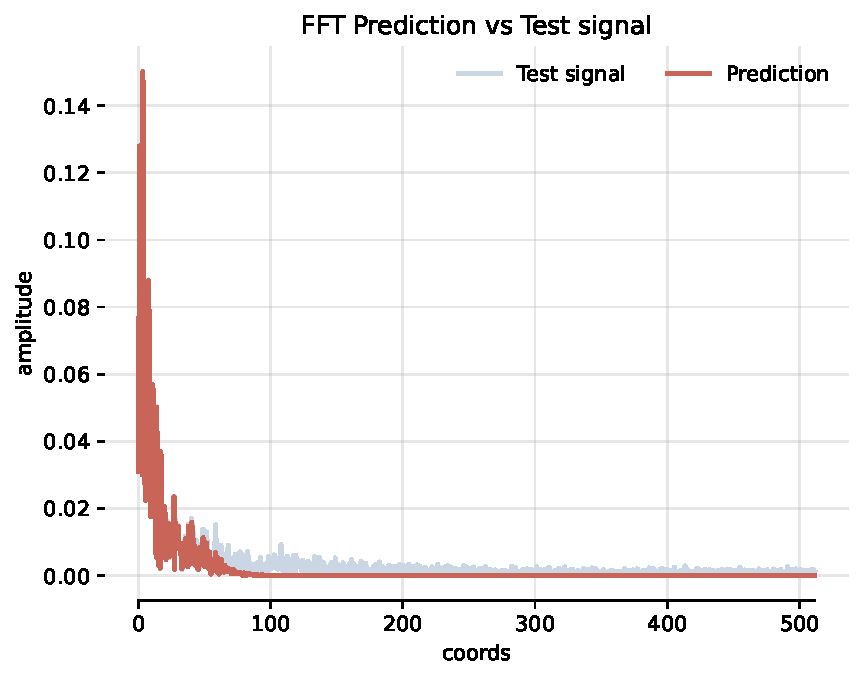
\includegraphics[width=\textwidth]{img/ch3/fft-noise-1hl-32hf-w8.pdf}
        \caption{}
        \label{fig:fft-noise-1hl-32hf-w8}
    \end{subfigure}
    \caption{Smoothed reconstruction with 1 hidden layer}
    \label{f:rec-1hl-32hf-8hz}
\end{figure}

The result in Figure \ref{fig:pred-noise-1hl-32hf-w8} resembles a smoothed version of the input signal, as expected, which is more evident in the zoomed-in view (Figure \ref{fig:4x-zoom-noise-1hl-32hf-w8}). However, the Fast Fourier Transform in Figure \ref{fig:fft-noise-1hl-32hf-w8} shows frequencies much higher than 8 Hz, in contrast to the shallow network experiments shown in Figures \ref{fig:rec-noise-shallow-w8} and \ref{fig:fft-noise-shallow-w8}. The FFT of the reconstructed signal aligns with that of the original signal up to around 30 Hz but fails to capture frequencies precisely within the range up to 100 Hz. Moreover, it does not show contributions from frequencies higher than 100 Hz.

Decreasing the number of neurons per layer slightly reduces the highest frequencies learned by the network, while increasing the network width allows it to capture higher frequencies, as demonstrated in Figure \ref{f:comparison-16-32-64-hf}. This can be observed in the FFT plots (Figures \ref{fig:fft-noise-1hl-16hf-w8}, \ref{fig:fft-noise-1hl-32hf-w8} and \ref{fig:fft-noise-1hl-64hf-w8}), and can also be perceived in the most refined details in the spatial reconstruction of the signal (Figures \ref{fig:4x-zoom-noise-1hl-16hf-w8}, \ref{fig:comp-4x-zoom-noise-1hl-32hf-w8} and \ref{fig:4x-zoom-pred-noise-1hl-64hf-w8}).

\begin{figure}[!h]
    \centering
    \begin{subfigure}[b]{0.32\textwidth}
        \centering
        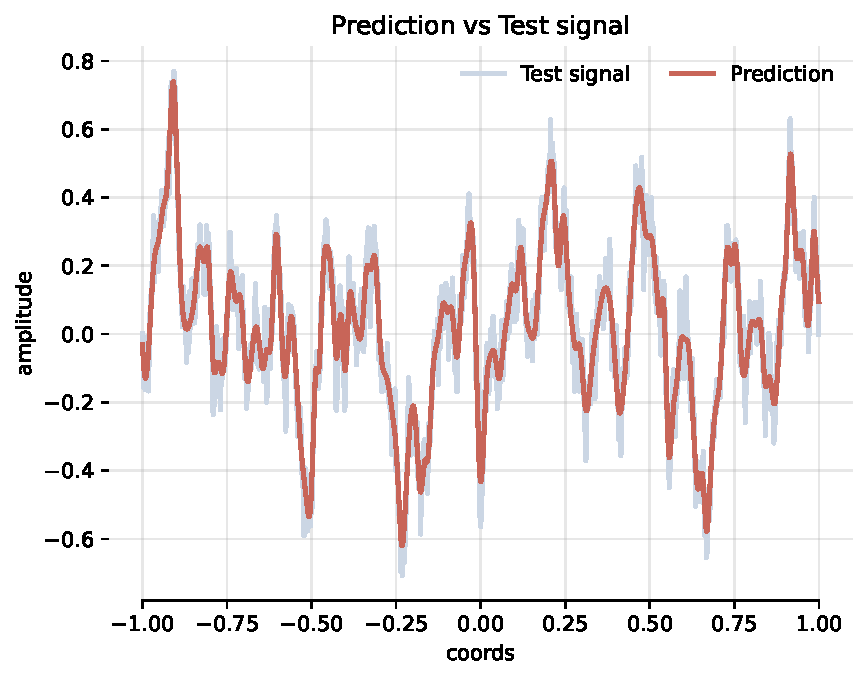
\includegraphics[width=\textwidth]{img/ch3/pred-noise-1hl-16hf-w8.pdf}
        \caption{16 neurons}
        \label{fig:pred-noise-1hl-16hf-w8}
    \end{subfigure}
    \begin{subfigure}[b]{0.32\textwidth}
        \centering
        \includegraphics[width=\textwidth]{img/ch3/pred-noise-1hl-32hf-w8.pdf}
        \caption{32 neurons}
        \label{fig:comp-pred-noise-1hl-32hf-w8}
    \end{subfigure}
    \begin{subfigure}[b]{0.32\textwidth}
        \centering
        \includegraphics[width=\textwidth]{img/ch3/pred-noise-1hl-64hf-w8.pdf}
        \caption{64 neurons}
        \label{fig:pred-noise-1hl-64hf-w8}
    \end{subfigure}

    \begin{subfigure}[b]{0.32\textwidth}
        \centering
        \includegraphics[width=\textwidth]{img/ch3/4x-zoom-noise-1hl-16hf-w8.pdf}
        \caption{16 neurons}
        \label{fig:4x-zoom-noise-1hl-16hf-w8}
    \end{subfigure}
    \begin{subfigure}[b]{0.32\textwidth}
        \centering
        \includegraphics[width=\textwidth]{img/ch3/4x-zoom-noise-1hl-32hf-w8.pdf}
        \caption{32 neurons}
        \label{fig:comp-4x-zoom-noise-1hl-32hf-w8}
    \end{subfigure}
    \begin{subfigure}[b]{0.32\textwidth}
        \centering
        \includegraphics[width=\textwidth]{img/ch3/4x-zoom-noise-1hl-64hf-w8.pdf}
        \caption{64 neurons}
        \label{fig:4x-zoom-pred-noise-1hl-64hf-w8}
    \end{subfigure}

    \begin{subfigure}[b]{0.32\textwidth}
        \centering
        \includegraphics[width=\textwidth]{img/ch3/fft-noise-1hl-16hf-w8.pdf}
        \caption{16 neurons}
        \label{fig:fft-noise-1hl-16hf-w8}
    \end{subfigure}
    \begin{subfigure}[b]{0.32\textwidth}
        \centering
        \includegraphics[width=\textwidth]{img/ch3/fft-noise-1hl-32hf-w8.pdf}
        \caption{32 neurons}
        \label{fig:comp-fft-noise-1hl-32hf-w8}
    \end{subfigure}
    \begin{subfigure}[b]{0.32\textwidth}
        \centering
        \includegraphics[width=\textwidth]{img/ch3/fft-noise-1hl-64hf-w8.pdf}
        \caption{64 neurons}
        \label{fig:fft-noise-1hl-64hf-w8}
    \end{subfigure}
    \caption{Comparison between different network widths}
    \label{f:comparison-16-32-64-hf}
\end{figure}

If we keep the width of the network fixed and increase the range of frequencies used in the initialization, the network can gradually capture higher frequencies. This continues until the network reaches its capacity, after which performance degrades, and the output turns into noise. Figure \ref{f:comparison-8-to-256-hz} illustrates this phenomenon with a network of 32 neurons per layer. Notice that from 8 Hz to 64 Hz, the network gets better in capturing finer details of the signal. However, when $\omega_0=128$, the reconstruction presents peaks and valleys bigger than those present in the signal, an indicative of spurious frequencies. By $\omega_0=256$, the result totally degenerates into noise.

\begin{figure}[h]
    \centering
    \begin{subfigure}[b]{0.32\textwidth}
        \centering
        \includegraphics[width=\textwidth]{img/ch3/16x-zoom-1hl-32hf-8hz.pdf}
        \caption{$\omega_0=8$}
        \label{fig:16x-zoom-1hl-32hf-8hz}
    \end{subfigure}
    \begin{subfigure}[b]{0.32\textwidth}
        \centering
        \includegraphics[width=\textwidth]{img/ch3/16x-zoom-1hl-32hf-16hz.pdf}
        \caption{$\omega_0=16$}
        \label{fig:16x-zoom-1hl-32hf-16hz}
    \end{subfigure}
    \begin{subfigure}[b]{0.32\textwidth}
        \centering
        \includegraphics[width=\textwidth]{img/ch3/16x-zoom-1hl-32hf-32hz.pdf}
        \caption{$\omega_0=32$}
        \label{fig:16x-zoom-1hl-32hf-32hz}
    \end{subfigure}

    \begin{subfigure}[b]{0.32\textwidth}
        \centering
        \includegraphics[width=\textwidth]{img/ch3/16x-zoom-1hl-32hf-64hz.pdf}
        \caption{$\omega_0=64$}
        \label{fig:16x-zoom-1hl-32hf-64hz}
    \end{subfigure}
    \begin{subfigure}[b]{0.32\textwidth}
        \centering
        \includegraphics[width=\textwidth]{img/ch3/16x-zoom-1hl-32hf-128hz.pdf}
        \caption{$\omega_0=128$}
        \label{fig:16x-zoom-1hl-32hf-128hz}
    \end{subfigure}
    \begin{subfigure}[b]{0.32\textwidth}
        \centering
        \includegraphics[width=\textwidth]{img/ch3/16x-zoom-1hl-32hf-256hz.pdf}
        \caption{$\omega_0=256$}
        \label{fig:16x-zoom-1hl-32hf-256hz}
    \end{subfigure}
    \caption{Comparison between different ranges of frequencies in initialization}
    \label{f:comparison-8-to-256-hz}
\end{figure}


% We observe that as we increase the value of $\omega_0$, meaning the frequency interval used in initialization of the first layer of the sinusoidal network, it becomes better in fitting fine details of the signal. Figure \ref{f:zoomed-views-noise} shows some zoomed views of the reconstruction. The grid where the network has been evaluated \red{has been refined XX, XXX and XXXX times}. Note that the model is well behaved in the points that were not given as supervision (not part of the training data), that is, it correctly interpolates the signal.


% On the other hand, if $\omega_0$ is too high it may cause the training to diverge. \red{In the Figure \ref{f:diverging-omega0}, we show the evolution of the training loss (Figure \ref{fig:diverging-loss}) and the result (Figure \ref{fig:diverging-reconstruction}) after 200 epochs when we initialized the SIREN with $\omega_0=600$. Note that after about 50 epochs, the loss starts to increase and our final result bears no resemblance to the original signal.}

We conclude that the frequency initialization of the first layer, which depends on $\omega_0$, is of central importance in the convergence of network training and frequency bands learning. In deep architectures, determining the upper bound of the frequencies learned is more complex compared to shallow architectures. However, we observe that the network can still progressively learn the lowest-frequencies of the signal up to a threshold defined by the choice of $\omega_0$.

Ideally we should initialize the network with frequencies that match the frequency content of the target signal. However, as we do not have access to this information in many applications, we must guess a value for $\omega_0$. The Shannon-Nyquist therorem may help us bound the value of $\omega_0$ in this task. For example, assuming that the signal is band-limited and considering a sampling rate of 1024 Hz, we cannot represent frequencies higher than 512 (half the sampling rate), so it does not make sense to choose $\omega_0$ higher than this value. Also, since the composition of sines generates much higher frequencies as consequence of a harmonic expansion (\cite{novello2022understanding}), it is reasonable to initialize the network with frequencies that are much lower than the Nyquist limit, and the experiments corroborate that.

% Another point worth noticing is that if the initialization frequencies are too high, the hidden layers may generate even higher frequencies, and even a model with high capacity will introducing noise into the model's reconstruction. This noise is not evident at the training coodinates, as the model overfits this data well, but it can be observed in a more refined grid FIGURE XXXX.}

\pagebreak

\subsection{Capacity Filtering}

The experiment illustrated in Figure \ref{f:comparison-16-32-64-hf} suggests that a network's capacity can serve as a filter when learning a signal. To further investigate this behavior, we compared the reconstruction of a stochastic signal using two networks: one with 16 neurons per layer and another with 256 neurons per layer. For this experiment, we generated a new Perlin noise signal with the following parameters: scale = 10, octaves = 14, and persistence = 1.5. Both networks have a single hidden layer and were initialized with $\omega_0=2$ Hz. The results are shown in Figure \ref{f:capacity-filter-16-hf-256}. 

\begin{figure}[h]
    \centering
    \begin{subfigure}[b]{0.32\textwidth}
        \centering
        \includegraphics[width=\textwidth]{img/ch3/pred-1hl-16hf-2hz.pdf}
        \caption{16 neurons}
        \label{fig:pred-1hl-16hf-2hz}
    \end{subfigure}
    \begin{subfigure}[b]{0.32\textwidth}
        \centering
        \includegraphics[width=\textwidth]{img/ch3/16x-zoom-1hl-16hf-2hz.pdf}
        \caption{16 neurons}
        \label{fig:16x-zoom-1hl-16hf-2hz}
    \end{subfigure}
    \begin{subfigure}[b]{0.32\textwidth}
        \centering
        \includegraphics[width=\textwidth]{img/ch3/fft-1hl-16hf-2hz.pdf}
        \caption{16 neurons}
        \label{fig:fft-1hl-16hf-2hz}
    \end{subfigure}

    \begin{subfigure}[b]{0.32\textwidth}
        \centering
        \includegraphics[width=\textwidth]{img/ch3/pred-1hl-256hf-2hz.pdf}
        \caption{256 neurons}
        \label{fig:pred-1hl-256hf-2hz}
    \end{subfigure}
    \begin{subfigure}[b]{0.32\textwidth}
        \centering
        \includegraphics[width=\textwidth]{img/ch3/16x-zoom-1hl-256hf-2hz.pdf}
        \caption{256 neurons}
        \label{fig:16x-zoom-1hl-256hf-2hz}
    \end{subfigure}
    \begin{subfigure}[b]{0.32\textwidth}
        \centering
        \includegraphics[width=\textwidth]{img/ch3/fft-1hl-256hf-2hz.pdf}
        \caption{256 neurons}
        \label{fig:fft-1hl-256hf-2hz}
    \end{subfigure}
    \caption{Comparison of reconstructions using networks with a single hidden layer and varying capacities.}
    \label{f:capacity-filter-16-hf-256}
\end{figure}

As expected, both networks produce smoothed versions of the input signal due to their initialization with low frequencies. However, the smaller network (top row) produces a significantly smoother reconstruction compared to the larger network (bottom row). This observation can be attributed to the smaller capacity of the network, which restricts it from learning higher frequencies. This highlights the role of network capacity as a natural frequency filter.

Previous work by \cite{Rahaman2018O} has demonstrated that during training, a Multi-Layer Perceptron (MLP) tends to learn lower frequencies before higher ones, a phenomenon known as spectral bias. Because sinusoidal neural networks are a form of MLP, this explains why, for a fixed depth, the network's width can act as a frequency filter. This capacity-based filtering effect, however, only holds if the network has sufficient capacity to capture the lower frequencies in the signal. As we increase the value of $\omega_0$ to capture higher frequencies, the network with 16 neurons per layer eventually becomes unable to fit the signal, and the reconstruction quality deteriorates. Figure \ref{f:capacity-filter-16hf-increasing-omega} provides zoomed-in views of reconstructions using a network with 16 neurons per layer initialized with different values of $\omega_0$. Notice how the reconstruction becomes progressively more detailed and closer to the input signal as $\omega_0$ increases, up to $\omega_0 = 32$. However, at $\omega_0=64$, the result degrades significantly.

\begin{figure}[h]
    \centering
    \begin{subfigure}[b]{0.32\textwidth}
        \centering
        \includegraphics[width=\textwidth]{img/ch3/16x-zoom-1hl-16hf-2hz.pdf}
        \caption{$\omega_0=2$ Hz}
        % \label{fig:pred-1hl-16hf-2hz}
    \end{subfigure}
    \begin{subfigure}[b]{0.32\textwidth}
        \centering
        \includegraphics[width=\textwidth]{img/ch3/16x_zoom-1hl-16hf-4hz.pdf}
        \caption{$\omega_0=4$ Hz}
        % \label{fig:16x-zoom-1hl-16hf-2hz}
    \end{subfigure}
    \begin{subfigure}[b]{0.32\textwidth}
        \centering
        \includegraphics[width=\textwidth]{img/ch3/16x_zoom-1hl-16hf-8hz.pdf}
        \caption{$\omega_0=8$ Hz}
        % \label{fig:fft-1hl-16hf-2hz}
    \end{subfigure}

    \begin{subfigure}[b]{0.32\textwidth}
        \centering
        \includegraphics[width=\textwidth]{img/ch3/16x_zoom-1hl-16hf-16hz.pdf}
        \caption{$\omega_0=16$ Hz}
        % \label{fig:pred-1hl-256hf-2hz}
    \end{subfigure}
    \begin{subfigure}[b]{0.32\textwidth}
        \centering
        \includegraphics[width=\textwidth]{img/ch3/16x_zoom-1hl-16hf-32hz.pdf}
        \caption{$\omega_0=32$ Hz}
        % \label{fig:16x-zoom-1hl-256hf-2hz}
    \end{subfigure}
    \begin{subfigure}[b]{0.32\textwidth}
        \centering
        \includegraphics[width=\textwidth]{img/ch3/16x_zoom-1hl-16hf-64hz.pdf}
        \caption{$\omega_0=64$ Hz}
        % \label{fig:pred-1hl-16hf-64hz}
    \end{subfigure}
    \caption{Comparison of reconstructions using a small network with varying values of $\omega_0$. 16x zoomed-in views.}
    \label{f:capacity-filter-16hf-increasing-omega}
\end{figure}

\section{Training, Generalization and Representation}
\label{sec:generalization}

% \red{We have established that we can bound the frequencies learned by a sinusoidal neural network by adjusting the interval of frequencies sampled for initialization of its first layer, and also by adjusting the network capacity. That is, if the value of $\omega_0$ is too low, the network will learn the lower frequencies of the signal, fitting their intensities in the Fourier spectrum, but won't learn the higher frequencies, even if it has enough computational units to to do. On the other hand, if the capacity given by the computational units is too small, the result will also resemble a filtered version of the target signal. TALVEZ MOVER PARA O CHAPTER 4 - MR-TRAINING}

Neural networks have been extensively used as analysis tools, as models trained in large datasets to recognize patterns and construct features to specific data types. However, we are using coordinate-based neural networks to represent signals. Our dataset is only 1 signal, or better saying, it is a set of samples of this signal, for example, a discrete set of coordinates and values. 

Some people say \red{trazer referências} that this is equivalennt to overfit a neural network to the signal, but we do not think this is the appropriate way to frame the problem. We want the neural network to be a continuous representation of a signal for which we only know a limited amount of samples. We actually need to solve a problem of  sampling and reconstruction, a classical problem in signal processing, guaranteeing that the neural representation contains the samples but also that it is "well behaved" in between. That means that when thinking of overfitting and generalization, we should borrow the perspective of regression problems and interpolation. For example, in polynomial interpolation it is known that high-degree polynomials will oscilate a lot, inclusing in regions between the interpolated points.

In this section, we investigate how well sinusoidal neural networks generalize to represent signals. To this end, we run experiments trying to reconstruct a signal from a critically sampled representation. For this, we take an input signal and we compute its Gaussian pyramid representation, that is, we filter the signal with a low-pass filter and subsample it by a factor of 2, repeating this procedure several times. We use these subsampled signals as training data for our experiments. 

On the other hand, additionally, we build a Gaussian Tower, that is, a filtered representation without decimation. To compensate for the lack of subsampling, we double the window of the filter for each level of the tower. This way, for a signal like a high frequency Perlin noise, the original signal is critically sampled, but the other levels of the Gaussian Tower are oversampled. According to the signal processing theory, for each level, it should be possible to perfectly reconstruct teh signal using only the samples in the Gaussian Pyramid. This way, we train the network in a Gaussian pyramid signal and we evaluate it against its correspondent in the Gaussian Tower. By sampling the network in a much more refined grid, and having a baseline to compare, we can verify if it is accuratelly representing the signal or if it is overfitting, that is, learning how to perfectly fit the samples, but introducing spurious frequencies and oscilating in between the supervised points.

For the next experiments, we generate another Perlin noise with the following parameters: scale: 10; octaves: 8; persistence: 0.9.



% - Present the experiments in fitting multiresolution signals
%     - 1D Gaussian Tower
%     - 1D Gaussian Pyramid
%     - show that networks is well behaved between samples

% \subsection{Gaussian Pyramid Training}


% After exploring the impact of different values of initialization frequencies, we investigated if we could fit multiple scales of the same signal by building a Gaussian pyramid of it. We filtered the signal using a box filter of dimension 5, decimated it by a factor of 2 and used this subsampled version to train our network. Then, we used the trained network to predict the values over all originally sampled points, so we could verify its behaviour on unsupervised points. As we are filtering the higher frequencies of the signal, we expect to be able to represent it exactly by using fewer samples, acconding to the classical sampling theory.  
% We compared our result to a smoothed but not decimated version of the signal where we doubled the size of the filter as we walked to coarse scales. The panel of figures below shows the result of fitting a signal in 7 different scales, starting with \omega_0=256 and dividing it by 2 as we walk to coarse scales.
% We trained the network using less points at each scale.

% \begin{figure}[!htb]
% \minipage{0.49\textwidth}
% \includegraphics[width=\linewidth]{charts/Section-20-Panel-0-ulotlhctz}
% \caption{}
% \endminipage\hfill
% \minipage{0.49\textwidth}
% \includegraphics[width=\linewidth]{charts/Section-20-Panel-1-twwld6gku}
% \caption{}
% \endminipage
% \end{figure}


% \chapter{Multiresolution Sinusoidal Neural Networks}
% \label{ch:mrnet}

% In recent years, the computer science community has seen an explosion in research in neural networks, motivated mainly by advances in Deep Learning~\cite{lecun2015deep,goodfellow2016deep}.
% For visual computing, this was spurred by the creation of Convolutional Neural Networks~(CNNs)~\cite{cnn98}, which had a significant impact both for the research community and the society at large~\cite{li2021survey,shamsaldin2019study}.
% The effectiveness of CNNs comes from the translation invariant properties of the convolution operator, which makes it a proper architecture for the analysis of visual imagery.

% Deep neural networks such as CNNs, employ an array-based discrete representation of the underlying signal. In this case, the network input consists of a vector of pixel values (in RGB) representing the image \emph{directly} by data samples. We call this kind of network a \textit{data-based} network.


% Moreover, the revolution in the media industry caused by deep neural networks motivated the development of new image representations using neural networks. While the data-based network is appropriate for analysis tasks, relying on a discretization of the image, another kind of network called \textit{coordinate-based~network} is suitable for synthesis, and provides a continuous and compact representation. For its characteristics, there is a growing interest in using these networks in imaging applications~\cite{xie2022neural}.
% For instance, coordinate-based networks have been successfully applied in image compression~\cite{dupont2021coin} and super-resolution~\cite{czerkawski2021neural}.


% A coordinate-based network represents the image \emph{indirectly} using a fully connected \textit{multi-layer perceptron} (MLP) that takes as input a pixel coordinate and outputs a RGB color. These~networks provide a continuous implicit representation for images~\cite{chen2021learning}, and allow for various applications, from Neural Signed Distance Functions~(NeuralSDFs)~\cite{park2019deepsdf} to Neural Radiance Fields~(NeRFs)~\cite{mildenhall2021nerf}. Since the coordinates are continuous, images can be presented in arbitrary resolution.

% % Sinusoidal neural networks are particularly suited to model stationary or quasi-stationary signals due to the periodic nature of its activation function~\cite{chen2022}.

% Sinusoidal neural networks are examples of coordinate-based networks in which their activation function is the sine function. As such, they bridge the gap between the spatial and spectral domains, given the close relationship of the sine function with the Fourier~basis. However, these sinusoidal neural networks have been regarded as difficult to train~\cite{taming2017}. To overcome this problem, \citet{sitzmann2019siren} proposed a sinusoidal network for signal representation called SIREN. One of the key contributions of this work is the initialization scheme that guarantees stability and good convergence. Furthermore, it also allows modeling fine details in accordance with the signal’s frequency content.

% A \textit{multiplicative filter network} (MFN) is a sinusoidal network simpler than SIREN which is equivalent to a shallow sinusoidal network~\cite{fathony2020multiplicative}. \citet{bacon2021} presented \textit{band-limited coordinate network }(BACON), an MFN that produces intermediate outputs with an analytical spectral bandwidth (specified at initialization) and achieves multiresolution of the underlying signal. While its structure allows BACON to be expressed as a linear combinations of sines, avoiding the composition of sines present in sinusoidal MLPs, it creates multiresolution representations by truncating the frequency spectra of the signals. This approach produces ringing artifacts  in some levels of detail, and becomes evident when we look at the Fourier transform of the images.

% The control of frequency bands in the representation is closely related with the capability of adaptive reconstruction of the signal in multiple levels of detail.
% In that context, \citet{mueller2022instant} developed a multiresolution neural network architecture based on hash encoding. Also, \citet{martel2021acorn} designed an adaptive coordinate network for neural signals.

% In this context, we introduce \textit{multiresolution sinusoidal neural networks}~(MR-Net) based on classical signal multiresolution representations. 
% Our results, presented in Section~\ref{sub:spectra-eval}, indicate that using MR-Net produces better results compared to the previous state-of-the-art technique, BACON, while employing a smaller number of parameters.
% We describe three MR-Net subclasses: S-Net, L-Net and M-Net.
% Finally, we present applications on antialiasing and level-of-detail reconstruction.

% - Related Works: Mip-Nerf; Bacon; 

\chapter{Multiresolution Sinusoidal Neural Networks}
\label{sec:mr_snn}

% This section presents \emph{multiresolution sinusoidal neural networks} (MR-Net) to represent signals in multiple levels of detail using sinusoisal MLPs.


\section{Overview of the MR-Net framework}

After studying and experimenting with sinusoidal neural networks, and developing an understanding of how the capacity and initialization of frequencies impact the frequencies learned by the network, we have designed a neural netwrok architecture to encode signals in multiresolution, leveraging classical multi-scale theory and modern deep learning techniques.

Our proposal is a family of coordinate-based networks with an unified architecture, and a framework for training neural networks on multiscale signal representation. We derive three main subclasses of MR-Nets: \emph{S-Net}, \emph{L-Net}, and \emph{M-Net}. Each of them offers different trade-offs in terms of frequency control in the signal representation.

The characteristics of the MR-Net framework are:

\begin{itemize}

\item Flexible training data -- the input signal can be given either by regular sampling, by multiresolution structure such as pyramids, or by stochastic / stratified sampling.

\item 2 Types of Level of Detail -- when training with multiresolution data, the level of details are determined by spectral projections, whereas with a single-resolution input signal, the level of details are determined by the network capacity.

\item Progressive Training -- the network is trained progressively, each stage at a time, using a variety of schedule regimes.

\item Continuous Multiscale -- the representation is continuous both in space and scale. Therefore, it can reconstruct the signal at any desired resolution / level of detail.
\end{itemize}


The next sections present the motivations and concepts underlying our approach, as well as the MR-Net architecture.

\section{Motivation}
\label{s-motivation}
Let $\gt{f}:\mathcal{D}\to \mathcal{C}$ be a \textit{signal}, the \textit{ground-truth}, where $\mathcal{D}$ and $\mathcal{C}$ are finite vector spaces representing the domain and codomain of~$\gt{f}$. For instance, to represent an image, we can choose $\mathcal{D}=\R^2$ to represent the image's support and $\mathcal{C}=\R^3$ to represent the RGB \textit{color space}.
Throughout the text, the cursive letter will indicate the ground-truth while the standard letter indicates the corresponding neural network.


We can decompose the signal into a sum $\gt{f}=\gt{g}_0+\dots+\gt{g}_{N-1}$ of $N$ stages, where $\gt{g}_0$ is its coarsest approximation and $\gt{g}_i$, for $i>0$, progressively introduce finer details. The \textit{level of detail}~$i$ is defined as 
$\gt{f}_i\!=\!\gt{g}_0\!+\!\cdots\!+\!\gt{g}_{i}$, or as 
$\gt{f}_i\!=\!\gt{f}\!-\left(\gt{g}_{i+1}\!+\!\cdots\!+\!\gt{g}_{N-1}\right)$. 
Thus, the stages can be defined as
$$\gt{g}_i=\gt{f}_{i+1}-K*\gt{f}_{i+1}, \text{ with } \gt{f}_{N-1}=\gt{f}.$$

That is, each stage $\gt{g}_i$ is the difference between the level $i+1$ and its convolution with a low-pass filter $K$. For example, $K$ could be a \textit{Gaussian kernel} $G(x,t)=\frac{1}{2\pi t}\exp{(-\frac{\norm{x}^2}{2t})}$, where $t$ is the scale parameter. The sequences $\{\gt{f}_i\}$ and $\{\gt{g}_i\}$ resemble the \textit{Gaussian} and \textit{Laplacian pyramids}, which are widely used in the multiresolution analysis of digital images~\cite{rosenfeld2013multiresolution,lindeberg1994scale,velho2009image}.

We address the problem of representing a signal $\gt{f}$ in multiresolution using sinusoidal neural networks. Motivated by the decomposition $\gt{f}=\gt{g}_0+\dots+\gt{g}_{N-1}$, we consider an aggregation of $N$ sinusoidal MLPs $g_i:\mathcal{D}\to \mathcal{C}$, which we call stages, to approximate $\gt{f}$. Therefore, we propose training each network stage $g_i$ by fitting it to the stages $\gt{g}_i$ of $\gt{f}$. This approach allows us to learn the frequency of $\gt{f}$ in a controlled manner, starting from lower details and gradually moving towards higher ones.
This is also inspired by the fact that MLPs tend to learn lower frequencies first, a phenomenon known as \emph{spectral bias}~\cite{Rahaman2018O}. 
We use a specific initialization of each network $g_i$ to control its capacity such that we can fit it to the stages $\gt{g}_i$ of $\gt{f}$.

% and as the training advances we add the the stages advances we consider 

% use the  that increasing the network depth (for fixed width) improves the network’s ability to fit higher frequencies, while increasing the width (for fixed depth) also helps, but the effect is considerably weaker.



\subsection{MR-Net Architecture}

We define the MR-Net as a function $f:\mathcal{D}\times [0,N]\to \mathcal{C}$, expressed as follows:
\begin{align}\label{e-mrnet}
f(x,t) = c_0(t)g_0(x) + \cdots + c_{N-1}(t)g_{N-1}(x),
\end{align}
Each function $g_i:\mathcal{D}\to\mathcal{C}$ is a sinusoidal MLP (see Sec~\ref{s-mr-module} for its precise definition) and represents the $i$th \textit{stage} of $f$, whose contribution is controlled by the function 
\begin{align}\label{e-control}
c_i(t)=\max\Big\{0, \min\big\{1, t-i\big\}\Big\}.
\end{align}
Note that when $t<i$, $c_i(t)=0$; when $i\leq t\leq i+1$, $c_i(t)=t-i$; and when $t>i+1$, $c_i(t)=1$.
Therefore, if $t=k+\delta$ with $k\in\mathbb{N}$ and $0\leq\delta\leq 1$, we obtain $$f(x,t)=g_0(x)+\dots + g_k(x)+\delta g_{k+1}(x).$$ 
$f_t:=f(\cdot, t):\mathcal{D}\to \mathcal{C}$ is the \textit{level of detail} $t$ of the MR-Net~$f$.
These levels evolve continuously, allowing us to encode a continuous multiresolution of $f$ at full resolution $f_N\!=\!g_0+\cdots + g_{N-1}$.
For this, we propose fitting $f$ to the multiresolution given by the ground-truth signal $\gt{f}=\gt{g}_0+\dots+\gt{g}_{N-1}$.
We initialize the parameters of each stage $g_i$ with sufficient capacity to fit the stage $\gt{g}_i$ (see Sec~\ref{s-frequency-control}), then train each $g_i$ to approximate $\gt{g}_i$.

The resulting MR-Net $f$ learns the decomposition of the ground-truth signal $\gt{f}$ as a projection into the coarse scale space and a sequence of finer detail spaces. For instance, the initial stage $f_1=g_0$ provides the least detailed approximation~of~$f_N$. The subsequent stages, represented by $g_i$ with $i<0$, progressively introduce finer details and are regulated by the scale parameter $t$. 
Essentially, the multiresolution can be navigated using the scale parameter $t$ within the interval $[0,N]$, which makes this architecture closely aligned with the Multiresolution Analysis~\cite{mallat-mr89}. Fig~\ref{f:mrnet-arch} shows the structure of a MR-Net having $N$ stages. 

\begin{figure}[!h]
\centering
\includegraphics[width=0.96\linewidth]{img/ch4/mr-net-stages-v2.png}
\caption{Anatomy of the MR-Net Family.}
\label{f:mrnet-arch}
\end{figure}



% The stages of the network are trained based on a predefined schedule (see Section~\ref{s:training}).
% During training, the control layer is the identity function, i.e. $\alpha = 1$.  


% The contributions of these $N$ stages are added together forming the network output.
% Assuming that the MR-Net is learning a function $f(x)$ that fits the input signal, then
% \begin{equation}
%     f(x) = g_0(x) + \cdots + g_{N-1}(x)
% \end{equation}
% where $g_i(x)$ is the detail function representing the stage $i$.
% The first stage $g_0$ gives the coarsest approximation of the signal and the other subsequent stages add increasingly finer details to it.





% Note that this architecture is very much in the spirit of the Multiresolution Analysis~\cite{mallat-mr89}. Indeed, consider the base case with $f = g_0 + g_1$, then $g_1 = f - g_0$, i.e. $g_1$ are the details that need to be added to $g_0$ to increase the level of detail.

% \hl{MR-Net learns the decomposition of the signal as a projection into the coarse scale space and a sequence of finer detail spaces.}


\subsection{MR Module}
\label{s-mr-module}
Each stage $g_i$ of the MR-Net $f$ is a sinusoidal MLP, called \textit{MR-Module}, that learns a signal representation as a combination of sinusoidal functions with induced frequency band.

We write each stage as $g_i=L_i\circ H_i\circ S_i$. The first layer projects the input $x$ into a list of sines $S_i(x)$, which is the input of the composition $H_i$ of the MLP hidden layers. The output $H_i\circ S_i(x)$ is a dictionary of sine combinations that are passed to the linear layer $L_i$. Finally, the control layer $c_i(t)$, with $t\in[i,i+1]$, blends the stage $g_i$ with the level of detail $f(x,i-1)$. 

There are two kinds of MR-Modules: \emph{Pure sine} MR-Module ($H_i=\emptyset$) and \emph{modulated sine} MR-Module ($H_i\neq\emptyset$). In the first case the network has only the first layer and the linear layer, and in the second case the network has the three blocks, including the hidden layers (see Fig~\ref{f:mr-module}).

\begin{figure}[!h]
\centering
% \includesvg[width=\linewidth]{svg_figs/diagram_mrnet.svg}
\includegraphics[width=\linewidth]{img/ch4/diagram_mr_module.pdf}
\caption{General Anatomy of a MR-Module.}
\label{f:mr-module}
\end{figure}

Without loss of generality, let us assume that the ground-truth signal is a grayscale image unless stated to the contrary. In this case, the stages of the MR-Net will have $\R^2$ and $\R$ as domain and codomain respectively. 
Consequently, a MR-Net with $N$ stages $g_i:\R^2\to \R$ has the form $f:\R^2\times [0,N]\to \R$.
Under this assumption, we present the building blocks of the MR-Net with details. 


\subsubsection{Pure Sine MR-Module}

The pure sine MR-Module is a shallow sinusoidal MLP defined as the composition $L\circ S$ of a sinusoidal layer $S$ with a linear layer $L$.
The layer $S\!:\!\R^2\!\to\! \R^m$ projects the input $x$ into a dictionary of $m$ sines of the form $S(x)=\sin\left(W_s x+ b_s\right)$, where $W_s\in \R^{m\times 2}$ and $b_s\in \R^{m}$ are the \textit{weight matrix} and \textit{bias}. The integer $m$ is the \textit{width} of the MR-Module.
The layer $L\!:\!\R^m\!\to\! \R$ is an affine map $L(x)=W_lx+b_l$, where $W_l\in \R^{1\times m} $ and $b_l\in \R$  are the final weight matrix and bias.
Hence, $L\circ S$ acts as a spectral filter controlled by the initialization of $W_s$.


Since the risk landscape for the network loss has many local minima, it is expected that the weights $W_s$ can’t move much further than their initialization. Therefore, $W_s$ determine the range of frequencies one can filter from the input signal. Fig~\ref{f:pure-sine} shows the structure of the $L\circ S$ and an example of a signal consisting of a linear combination of two frequencies. In this example, we have the layers $S\!:\!\R\!\to\! \R^2, S(x) = (sin(x), sin(5x))$ and $L\!:\!\R^2\!\to\! \R, L(x_1, x_2) = x_1 + x_2$.

\begin{figure}[!h]
\centering
\includegraphics[width=0.8\linewidth]{img/ch4/pure-sine.png}
\caption{Pure sine MR-Module.}
\label{f:pure-sine}
\end{figure}


\subsection{Modulated sine MR-Module}

The Modulated MR-Module is a deep sinusoidal MLP $L\circ H\circ S$ that considers a hidden sinusoidal layer block $H:\R^m\to~\R^m$. 
This map is the composition of $k$ layers $H=H_k\circ \dots \circ H_1$ with $H_i(x_i)\!=\!\sin\left(W_i x_i \!+\! b_i\right)\!=\!x_{i+1}$ where $x_0\!\in\!\R^m$ is the input.
The integers $m$ and $k+1$ are the \textit{width} and \textit{depth} of the MR-Module.  

The MR-Module $L\circ H\circ S$ is a linear combination of a dictionary of (spectral) atoms $H\circ S$ containing composition of sines. This fact has two consequences. First, the capacity of $L\circ H\circ S$ is greater than the capacity of $L\circ S$ with the same number of neurons~\cite{novello2022understanding}. Second, the initialization of $L\circ H\circ S$ does not directly control its frequency band as in the case of $L\circ S$.

In terms of localization properties in space and frequency, we can say the spectral atoms of the Modulated MR-Module are semi-local in the sense that these functions are adapted by the learning process to fit local variations of the signal (i.e., frequencies) across its (spatial) domain. This characteristic is evident in Fig~\ref{f:modulated} that shows a network structure and the graph of $\sin\Big(3\sin\big(5\sin(1.9x)\big)\Big)$.
In this example, the first layer is represented by $S(x)=\sin(1.9 x)$, the hidden block is the composition of two sine layers $H(x)=\sin\big(3\sin(5x)\big)$, and the linear layer is the identity function $L(x)=x$.

\begin{figure}[!h]
\centering
\includegraphics[width=0.9\linewidth]{img/ch4/modulated-sine.png}
\caption{Modulated sine MR-Module.}
\label{f:modulated}
\end{figure}



\section{MR-Net Subclasses}

Here, we describe three subclasses of the MR-Net: \emph{S-Net}, \emph{L-Net}, and \emph{M-Net}.
The characteristics of their level of details depend on the configuration of their stages. %, as will be presented next.
Recall, from Eq~\ref{e-mrnet}, that a MR-Net is a function $f:\R^2\times [0,N]\to \R$, expressed as:
\begin{align*}
f(x,t) = c_0(t)g_0(x) + \cdots + c_{N-1}(t)g_{N-1}(x).
\end{align*}
Therefore, to define the subclasses S-Net, L-Net, and M-Net, we only need to define the stages $g_i$.


\subsection{S-Net}

A S-Net is a MR-Net in which each stage $g_i$ is a pure sine MR-Module, i.e. $g_i=L_i\circ S_i$ where $S_i$ and $L_i$ are the first and the linear layers (see Fig~\ref{f:s-net}).
%
For this reason, each stage $g_i$ can be  
% consists of a learned ``sine transform'', with its layers corresponding, respectively, to the direct and inverse sine transform. Specifically, 
expressed as a sum of sine functions
$$g_i(x)=a_0+\sum_{j=1}^m a_j \sin\left(\omega_j x+\varphi_j\right),$$ where the \textit{frequencies} $\omega_j$ and \textit{phase-shifts} $\varphi_j$ are given by the weights and bias of the first layer $S_i$. The \textit{amplitudes} $a_j$ are given by the linear layer $L_i$.
%
As a consequence, the resulting S-Net $f$ can provide level of detail based on the controlled initialization of frequency band of each stage $g_i$ (see Sec~\ref{s-frequency-control}).
\begin{figure}[!h]
\centering
\includegraphics[width=0.58\linewidth]{img/ch4/snet.pdf}
\caption{S-Net architecture.}
\label{f:s-net}
\end{figure}

\subsection{L-Net}
\label{s-lnet}
A L-Net is a MR-Net $f$ in which each stage $g_i=L_i\circ H_i\circ S_i$ is an independent modulated sine MR-Module: $S_i$, $H_i$, $L_i$ are the first, hidden, and linear blocks (see Fig~\ref{f:l-net}).
%
For this reason, the level of detail capacity of $f$ is determined by the width and depth of each stage $g_i$.
% The first stage $g_0$ is the coarsest approximation of the underlying function.
\begin{figure}[!h]
\centering
\includegraphics[width=0.7\linewidth]{img/ch4/lnet.pdf}
% \vspace{-0.4cm}
\caption{L-Net architecture. Note that the stages are independent of each other.}
\label{f:l-net}
\end{figure}


The $N$th level $f(\cdot, N)$ of a L-Net is an example of a sinusoidal MLP.
Without loss of generality, let $f(\cdot, t)=~c_0(t)g_0+c_1(t)g_1$ be a L-Net with two stages having the same architecture with a single hidden layer. We show that $f(\cdot, 2)\!=\!L\!\circ\! H\!\circ\! S$.
For this, define the matrices of $S$, $H$, and $L$, respectively, using $W_s\!=\!\begin{psmallmatrix}W_s^0\\W_s^1\end{psmallmatrix}$, 
$W_h\!=\!\begin{psmallmatrix}W_h^0& 0\\0&W_h^1\end{psmallmatrix}$, 
$W_l\!=\!\begin{psmallmatrix}W_l^0 & W_l^1\end{psmallmatrix}$, where $W_s^j$, $W_h^j$, $W_l^j$ are the matrices of the stages~$g_j$. The biases are defined in a similar way. Such procedure can be extended to a sum of $N$ stages in a analogous way.
Thus, the L-Net gives us a controllable way of increasing the \textit{width} of a sinuoisal MLP during training.


\subsection{M-Net}
\label{s-mnet}
While the stages of S-Nets and L-Nets are independent, with M-Net we propose a way to reuse information learned at previous stages.
A M-Net is a MR-Net where each stage $g_i$ is a modulated MR-Module linked to its subsequent stage $g_{i+1}$.
That~is, $H_i\circ  S_i$ is composed both with the linear layer $L_i$, producing the stage $g_i\! =\! L_i\!\circ\! H_i\!\circ\!  S_i$, and the hidden block $H_{i+1}$ resulting in $g_{i+1}\! =\! L_{i+1}\!\circ H_{i+1}\!\circ\left(S_{i+1}, H_i\circ  S_i\right)$ (Fig~\ref{f:m-net}).
This way, the hidden block has the form $H_{i+1}\!:\!\R^{2m}\!\to\! \R^m$; $m$ is the number of neurons.
\begin{figure}[!h]
\centering
\includegraphics[width=0.75\linewidth]{img/ch4/mnet.pdf}
% \vspace{-0.4cm}
\caption{M-Net architecture. Notice how the hidden-layers blocks of adjacent MR-Modules are connected.}
\label{f:m-net}
\end{figure}

The hidden block of a stage of the M-Net is composed~with~a sequence of hidden blocks coming from previous stages.~That~is, the M-Net contains a deep MLP $L_{N-1} \circ \overline{H_{N-1}} \circ \cdots \circ \overline{H_1}\circ H_0 \circ S_0$ with $N$ hidden blocks; $\overline{H_i}$ is the part of $H_i$ connecting to the stage $g_{i+1}$.
Thus, the M-Net also allows us to increase the \textit{depth} of a sinusoidal MLP during training implying that the capacity of each stage increases with its depth in the hierarchy.
This feature makes the M-Net a suitable and compact architecture for  multiresolution training, as discussed in Sec~\ref{sec:considerations}, and we will utilize this subclass in the applications of Sec~\ref{s:img}.


\subsection{Frequency Control}
\label{s-frequency-control}

Let $\gt{f}=\gt{g}_0+\cdots+\gt{g}_{N-1}$ be the ground-truth signal in multiresolution, and $f:\R^2\times [0,N]\to \R$ be a MR-Net with $N$ stages. To train each stage $g_i$, we propose to initiate its parameters based on the frequency content of $\gt{g}_i$.
There are two ways to control the frequency band of $g_i$. First, we can initialize the weight matrix of the first layer of $g_i$. Second, we can vary its width and depth. Moreover, these mechanisms can be combined.


\subsubsection{Frequency Initialization}
\label{s-frequency-initialization}


Training sinusoidal MLPs can be challenging  as periodic activation functions may lead to instability in deep architectures~\cite{taming2017}. \citet{sitzmann2019siren} propose an initialization scheme that guarantee stability during training. 
They initialize the weights $W=\omega \, \tilde{W}$ of the MLP first layer $ \sin\left(Wx + b\right)$ such that $\tilde{W}$ is uniformly sampled in $[-1,1]$ and the number $\omega$ controls the range of frequencies. That is, the layer projects the input $x$ in a list of sines with frequencies in $[-\omega, \omega]$. 
They empirically choose $\omega=30$ in their experiments. For the hidden layers, they choose the weights distributed uniformly in $\left(-\sqrt{6/m}, \sqrt{6/m}\right)$, where $m$ is the width of the layer. See \cite{sitzmann2019siren} for the details.

Regarding the initialization of the MR-Net $f$, let $g_i=L_i\circ H_i\circ S_i$ be its $i$th stage, where $S_i$, $H_i$, and $L_i$ are its first, hidden, and linear blocks.
Observe that each coordinate of the sinusoidal layer $S_i(x)=\sin\left(W_{s_i} x+b_{s_i}\right)$ has the form $\sin(\omega_1 x_1 +\omega_2 x_2 + \varphi)$, where the \textit{frequencies} $\omega_1$ and $\omega_2$ form a line of the matrix $W_{s_i}$, $x=(x_1,x_2)$ is the input, and the \textit{phase-shift} $ \varphi$ is a coordinate of the bias $b_{s_i}$. We follow the above initialization approach to initialize $g_{i}$. However, instead of using $\omega=30$ we consider it to be a \textit{bandlimit frequency} on the ground-truth stage $\gt{g}_i$.

% The initialization of the elements of the matrix $W_{s_i}$ in the sinusoidal layer $S_i(x)=\sin\left(W_{s_i} x+b_{s_i}\right)$ is of central importance in the training convergence of $f$.

Ideally, the initialization of frequencies in $g_i$ should match the frequency content of the ground-truth signal at the stage $\gt{g}_i$. 
However, as we usually don't have access to this information, we opt to use an upper bound. 
Specifically, we assume that $\gt{g}_i$ has no frequency higher than a \textit{bandlimit} $B_i$. The Nyquist–Shannon sampling theorem says that we can reconstruct $\gt{g}_i$ from a sample $\{\gt{g}_i(x_{kl})\}$, where the regular grid $x_{kl}$ has points spaced with size $\frac{1}{r_i}<\frac{1}{2B_i}$. The number $r_i$ is the \textit{sample rate}. Fig~\ref{f:nyquist} illustrates such requirement using the frequency rate notation.  
% Assuming that the signal has been properly sampled, the ``Nyquist limit'' gives the maximum frequency contained in the signal, which is $\frac{1}{2} f_s$, where $f_s$ is the sampling rate (see Fig~\ref{f:niquist}).
\begin{figure}[!h]
\centering
\includegraphics[width=0.7\linewidth]{img/ch4/nyquist.png}
\vspace{-0.3cm}
\caption{Nyquist Limit.}
\label{f:nyquist}
\end{figure}


Therefore, to fit the stage $g_i$ to the sample $\{\gt{g}_i(x_{kl})\}$, we opt to initialize $g_i$ such that it can represent frequencies up to $\omega_i:=\frac{r_i}{2}$.
For this, we initialize the lines of the first matrix $W_{s_i}$ of $g_i$ uniformly in the set $\Omega_i=\left[-\omega_i, \omega_i\right]^2$.
Thus, the sinusoidal layer $S_i$ may contain frequencies already initialized at previous stages because $\{\gt{g}_i\}$ is a Laplacian pyramid of $\gt{f}$, thus, $\Omega_0\subset \cdots \subset \Omega_{N-1}$. The weights of the hidden block $H_i$ are initialized following the same scheme in \cite{sitzmann2019siren}.

% \vspace{0.2cm}
% {\color{red}
% In practice, we assume that the data is given as a regular sample (digital image) of size $2^{k}\times 2^k$
% of the ground-truth signal~$\gt{f}$.
% We abuse the notation by denoting this digital image by~$\gt{f}$.
% To train the MR-Net stages~$\{g_i\}$, we use the (discrete) \textit{Gaussian} and \textit{Laplacian} pyramids of $\gt{f}$, both with $N<k$ levels.
% Precisely, the Gaussian pyramid $\{\gt{f}_i\}$ is defined recursively by convolving the \textit{level of detail} $\gt{f}_i$ with a Gaussian kernel $K$ and downsampling the result by a factor 2:
% \begin{align*}
%     \gt{f}_i(k,l)&=\left(K*\gt{f}_{i+1}\right)(2k,2l)\,\, \text{with} \,\, k,l\in \left\{1,\ldots, 2^{k-N+1+i}\right\},\\
%     \gt{f}_{N-1}&=\gt{f}.
% \end{align*}
% $\gt{f}_i(k,l)$ denotes the digital image $\gt{f}_i$ evaluated at the pixel $(k,l)$.
% Similarly, the Laplacian pyramid $\{\gt{g}_i\}$ is defined using
% \begin{align*}
%     \gt{g}_i(k,l)&=\left(\gt{f}_{i}-K*\gt{f}_{i}\right)(2k,2l)\,\, \text{with} \,\, k,l\in \left\{1,\ldots, 2^{k-N+1+i}\right\}\\ \gt{g}_0(k,l)&=\left(K*\gt{f}_{1}\right)(2k,2l).
% \end{align*}
% Since $2^{k-N+1+i}$ is the height and width of $\gt{g}_i$, it cannot contain frequencies higher than $\omega_i=2^{k-N+i}$. 
% Thus we propose to initialize the frequencies of the $N$ stages $\{g_i\}$ of the MR-Net $f$ following a dyadic sequence of frequency bands 
% \begin{align}
% \omega_{N-1}, \omega_{N-2}, \ldots, \omega_{0}.
% \end{align}
% Which is equivalent to $\omega_{N-1}, \frac{\omega_{N-1}}{2}, \ldots, \frac{\omega_{N-1}}{2^{N-1}}$ with $\omega_{N-1}= 2^{k-1}$.
% These are the bandlimits used to define the sets $\Omega_i=\left[-\omega_i, \omega_i\right]^2$ to initialize the frequencies of the first layer of each stage $g_i$.
% (see Fig~\ref{f:freq-bands}).

% \begin{figure}[!h]
% \centering
% \includegraphics[width=0.98\linewidth]{figs/freq-bands.png}
% \caption{Frequency Bands}
% \label{f:freq-bands}
% \end{figure}

% }

% Finally, the training of each stage $g_i$ is done by minimizing the following loss functional
% \begin{align}
%     \mathscr{L}(\theta_i)=\sum_{k=1}^{2\omega_i}\sum_{l=1}^{2\omega_i}\Big(\gt{g}_i(k ,l)-g_i(k,l)\Big)^2
% \end{align}

\subsubsection{MR-Module Capacity}
\label{sec-module-capacity}

The capacity of each MR-Net stage $g_i=L_i\circ H_i\circ S_i$ is controlled by its width $m$ and depth $k+1$.
The width $m$ determines that an input $x$ will be transformed into a list of $m$ sines $S_i(x)=\sin\left(W_{s_i}x+b_{s_i}\right)$,
where $W_{s_i}$ has rows sampled at the set $\Omega_i$ defined in Section~\ref{s-frequency-initialization}. By increasing $m$, the dictionary of input frequencies is augmented. The hidden block $H_i$ consisting of $k$ sinusoidal layers, further enhances this list of frequencies.


To mitigate the effects of the spectral bias, we employ the above frequency initialization approach to the stage $g_i$. This ensures that the training of $g_i$ begins with frequencies that are \textit{close} to those present in the corresponding ground-truth data $\gt{g}_i$.
% See Fig~\ref{f:capacity}.
% \begin{figure}[!h]
% \centering
% \includegraphics[width=0.97\linewidth]{figs/width.png}\\
% \includegraphics[width=0.97\linewidth]{figs/depth.png}
% \vspace{-0.2cm}
% \caption{Capacity Hyperparameters (from~\cite{Rahaman2018O})}
% \label{f:capacity}
% \end{figure}

Furthermore, the MR-Net architecture enables us to gradually increase its width and depth by adding stages (see Secs~\ref{s-lnet} and \ref{s-mnet}), providing us with a controlled way of increasing network capacity while allocating ground-truth frequencies across stages in a controllable manner.
For example, a L-Net can be viewed as a specific MLP where adding a new stage increases its width. As a result, L-Net allows us to divide a given MLP into stages. On the other hand, M-Net has a more sophisticated structure, as adding a stage results in a network that is wider and deeper.


% \section{MR-Net in Detail}
% \label{sec:mrnet_detail}

This section presents the MR-Net framework in detail by conceptually dividing it in four main components: \emph{MR-Structure}, \emph{MR-Stages}, \emph{MR-Training}, and \emph{MR-Inference} (see Fig~\ref{f:components}). 

% Although coordinate-based networks could be applied to represent signals in other dimensions, as demonstrated by SIREN \cite{sitzmann2019siren} and BACON \cite{bacon2021}, we are going to focus on images, that is signals XXXXX, the applications described in section XXXXX. For 1D applications, please refer to XXXXX.

\begin{figure}[!h]
\centering
\includegraphics[width=0.99\linewidth]{img/ch4/mr-net-components.png}
\caption{MR-Net framework Components.}
\label{f:components}
\end{figure}

% Let $\gt{f}:\mathcal{D}\to \mathcal{C}$ be the ground-truth signal (\textit{input data}), and $f\!:\!\mathcal{D}\!\times\! [0,N]\!\to\! \mathcal{C}$ be a MR-Net with $N$ stages $\{g_i\}$ to fit $\gt{f}$~in multiresolution.
% We use this setting to present the framework.

\subsection{MR-Structure}\label{sec:mr_struct}

The MR-Structure is a data structure that encapsulates the input data $\gt{f}$. It includes $\gt{f}$ and metadata about its \textit{sampling mode}, \textit{filtering type}, and the \textit{multi-stage stack} (see Fig~\ref{f:structure}).
\begin{figure}[!h]
\centering
\includegraphics[width=0.89\linewidth]{img/ch4/mr-structure.png}
\caption{MR-Structure.}
\label{f:structure}
\end{figure}

% \subsubsection{Input Data}

The training of MR-Net stage $g_i$ receives pairs $\{x_j, y_j\}$ as input, with points $x_j$ sampled in the domain $\mathcal{D}$ of $\gt{f}$ and $y_j=\gt{f}(x_j)\in~\mathcal{C}$. For a squared image, we could have $\mathcal{D}=[-1, 1]^2 \subset \R^{2}$. During training, we consider the signal $\gt{f}$ to have codomain in monochromatic ($\mathcal{C}=\R$) or RGB color ($\mathcal{C}=\R^3$) (see Fig~\ref{f:values}). 
Depending on the application, other color spaces or additional attributes, such as masks and features, could be used (see Fig~\ref{f:attributes}). 
\begin{figure}[!h]
\centering
\includegraphics[width=0.8\linewidth]{img/ch4/attrib-d0-d1.png}
\caption{Image values (RGB and monochromatic).}
\label{f:values}
\end{figure}

\begin{figure}[!h]
\centering
\includegraphics[width=0.8\linewidth]{img/ch4/attrib-mask.png}
\caption{Examples of image attributes (mask and edges).}
\label{f:attributes}
\end{figure}


The data input for the training of each of the $N$ stages $g_i$ is organized in a \textit{multi-stage stack} $\{x_j, y_j\}_i$.
% consisting of a hierarchy of sampling grids. 
Specifically, for each $i$, the set of pairs $\{x_j, y_j\}_i$ is a sample of the $i$th level of detail $\gt{f}_i$ of the signal $\gt{f}$ or a sample of the original signal $\gt{f}$, with $\{x_j\}_i\subset \mathcal{D}$ and $\{y_j\}_i=\{\gt{f}_i(x_j)\}$. 
From the point of view of \textit{representation theory}, we can interpret this as a projection of the function $\gt{f}_i$ onto the primal \textit{Shannon basis} (i.e., Dirac delta distribution). In the context of signal processing, this basis is a sampling grid of impulses and the representation consists of the sequence $\{y_j\}_i$ at the grid locations $\{x_j\}_i$.

The type of sampling used to extract the multi-stage stack $\{x_j, y_j\}_i$ from the signal $\gt{f}$ is an important aspect in the MR-Net training. In that respect, it is instrumental to consider two types of samplings: \textit{regular} and \textit{irregular} (Fig~\ref{f:sampling}). 
%
In the regular case, the sampled points are organized in a regular grid discretization $\{x_{k,l}\}$ of the domain $\mathcal{D}$. 

% The irregular sampling consider the points $\{x_i\}$ to be uniformly sampled from $\mathcal{D}$.
% , i.e. for each pair $k,l$ we have $\norm{x_{k,l}-x_{k+1,l}}=\norm{x_{k,l}-x_{k,l+1}}=\Delta$ with $\Delta$ being a constant. 
%
For flexibility, we implement a sampler module that take regular samples or stochastic samples using the Poisson disk sampling~\cite{stochastic_cook, poisson_bridson}. 
The sampler could be extended to work with different sampling patterns. 
The sampling mode is stored in the MR-Structure, so it can be taken into account when doing operations that modify the sampling grid.

\begin{figure}[!h]
\centering
\includegraphics[width=0.45\linewidth]{img/ch4/regular.png}
\hfil
\includegraphics[width=0.45\linewidth]{img/ch4/poisson.png}
\\
{\small\hfil (regular grid) \hfil\hfil\hfil (irregular grid) \hfil}
\vspace{-0.2cm}
\caption{Sampling modes.}
\label{f:sampling}
\end{figure}


The multi-stage stack of the input signal $\gt{f}$ could have different resolutions.
For the regular case where the sampled points are organized in a regular grid $\{x_{k,l}\}$ (the highest resolution), we can structure the multi-stages in dyadic lattice following the $2^i$ rule: 
\begin{align*}
\{x_{k,l}\}_i=\{x_{2k,2l}\}_{i+1}\text{ with }\{x_{k,l}\}_N=\{x_{k,l}\}.
\end{align*}
Here we are assuming that $\{x_{k,l}\}$ is a grid of size $2^k\times 2^k$ for some integer $k>N$.
Thus each dimension of a stage grid $\{x_{k,l}\}_i$ has twice the size of the previous one (Fig~\ref{f:multi}(a)). 
On the other hand, we could consider that the sampling grids $\{x_{k,l}\}_i$ have a fixed resolution, and sample the signal $\gt{f}$ on its highest level or consider the level of detail $\gt{f}_i$ for each grid stage $\{x_{k,l}\}_i$ (Fig~\ref{f:multi}(b)). See Section~\ref{s:lod} for more details.
% Nonetheless, it is also possible to define a irregular multiresolution grid structure. In this case, each resolution level has approximately twice the number of random sample points of the previous level .
\begin{figure}[!h]
\centering
\begin{subfigure}{0.49\linewidth}
\includegraphics[width=\linewidth]{img/ch4/pyramid.png}
\caption{Pyramid}
\end{subfigure}
\begin{subfigure}{0.49\linewidth}
\includegraphics[width=\linewidth]{img/ch4/tower.png}    
\caption{Tower}
\end{subfigure}
\caption{Examples of multi-stage stacks.}
\label{f:multi}
\end{figure}

Each level $i$ of the multi-stage stack can be filtered to separate the level of detail $\gt{f}_{i+1}$ into different frequency bands. In this sense, we can use the unfiltered signal $\gt{f}$, a low-pass version of $\gt{f}_{i+1}$ or a band-pass version of $\gt{f}_{i+1}$. For this, it is common to employ a Gaussian kernel as the low-pass kernel and a difference of Gaussians as the band-pass kernel (see Fig~\ref{f:filter}).
Precisely, we can filter $\gt{f}_{i+1}$ by convolving it with a Gaussian kernel $K$:
% and downsampling the result by a factor 2:
\begin{align}\label{e-gaussian-filter}
    \gt{f}_i(k,l)&=\left(K*\gt{f}_{i+1}\right)(k,l)
\end{align}
We abuse the notation and denote by $\gt{f}_i(k,l)$ the function $\gt{f}_i$ evaluated at  $x_{k,l}$.
Similarly, the $i$th band-pass stage $\gt{g}_i=\gt{f}_i-\gt{f}_{i-1}$ is defined using $\gt{g}_i(k,l)=\left(\gt{f}_{i}-K*\gt{f}_{i}\right)(k,l)$.

\begin{figure}[!h]
\centering
\includegraphics[width=0.32\linewidth]{img/ch4/signal.png}
\includegraphics[width=0.32\linewidth]{img/ch4/gaussian.png}
\includegraphics[width=0.32\linewidth]{img/ch4/laplacian.png}\\
{\hfil \hfil signal \hfil \hfil \hfil low-pass \hfil \hfil \hfil band-pass \hfil}
\caption{Examples of filter types.}
\label{f:filter}
\end{figure}


% % \subsubsection{Sampling}
% % The input for the neural network is a discrete representation. In this sense,} sampling is a way to create a representation of a function based on its values at certain points of the domain. From the point of view of Representation Theory, we can interpret this as a projection of the function onto the primal Shannon basis (i.e., Dirac delta distribution). In the context of signal processing, this basis is a sampling grid of impulses and the representation consists of the sequence of signal values at the grid locations.

% % One important aspect of sampling for learning signals with coordinate-based neural network is the structure of the sampling grid. In that respect, it is instrumental to consider two types of grid structures: Regular and Irregular. See Fig~\ref{f:sampling}. {\color{red}The sampling mode is stored in the MR-Structure, so it can be taken into account when doing operations that modify the sampling grid.}

% % \begin{figure}[!h]
% % \centering
% % \includegraphics[width=0.42\linewidth]{img/ch4/regular.png}
% % \hfil
% % \includegraphics[width=0.42\linewidth]{img/ch4/poisson.png}
% % \\
% % {\hfil (regular grid) \hfil\hfil (irregular grid) \hfil}
% % \caption{Sampling Modes}
% % \label{f:sampling}
% % \end{figure}


% % \subsubsection{Filtering}

% % The input of signal values to the network can be filtered to separate it into different frequency bands. In this sense, we can use the unfiltered signal, a low-pass version of the signal or a band-pass version of the signal. See Fig~\ref{f:filter}.

% % It is common to employ a Gaussian Kernel as the low-pass Kernel and a Difference of Gaussians as the band-pass kernel.

% % \begin{figure}[!h]
% % \centering
% % \includegraphics[width=0.30\linewidth]{img/ch4/signal.png}
% % \includegraphics[width=0.30\linewidth]{img/ch4/gaussian.png}
% % \includegraphics[width=0.30\linewidth]{img/ch4/laplacian.png}\\
% % {\hfil \hfil signal \hfil \hfil \hfil low-pass \hfil \hfil \hfil band-pass \hfil}
% % \caption{Filter Types}
% % \label{f:filter}
% % \end{figure}

% % \subsubsection{multi-stage stack}

% % A Multiresolution Stack consists of a hierarchy of sampling grids with different resolutions. The standard grid structure form a dyadic lattice of regular grids obeying the $2^j$ rule, i.e., each level of the grid has twice the size of the previous one. 
% % Nonetheless, it is also possible to define a irregular multiresolution grid structure. In this case, each resolution level has approximately twice the number of random sample points of the previous level (see Fig~\ref{f:multi}(b)).
% % On the other hand, it is possible to have a stack of sampling grid with the same resolution, in which the signal is the same at each level or is filtered (see Fig~\ref{f:multi}(a)). Section~\ref{s:lod} gives more details on this option.
% % \begin{figure}[!h]
% % \centering
% % \includegraphics[width=0.45\linewidth]{img/ch4/tower.png}
% % \includegraphics[width=0.45\linewidth]{img/ch4/pyramid.png}\\
% % {\hfil tower \hfil \hfil \hfil pyramid \hfil}
% % \vspace{-0.2cm}
% % \caption{\hl{Multiresolution Hierarchies}}
% % \label{f:multi}
% % \end{figure}


\subsection{MR-Stages}\label{sec:mr_stages}

The MR-Stages $\{g_i\}$ are the build blocks of the MR-Net $f$. They constitute a stack of MR-Modules that are interconnected according to the chosen MR-Net subclass as illustrated on Figures ~\ref{f:s-net}, \ref{f:l-net}, and \ref{f:m-net}.

% \begin{figure}[!h]
% \centering
% \includegraphics[width=0.3\linewidth]{img/ch4/mr-stages.png}
% \caption{MR-Stages}
% \label{f:stages}
% \end{figure}

The MR-Net configuration is given by the 
parameters of the MR-Stages: number of stages, depth and width of the stages.


\subsection{MR-Training}\label{sec:mr_training}
\label{s:training}

The training of the MR-Net $f$ must consider the mechanisms for learning different levels of detail at each stage $g_i$ of $f$. 
The capacity of $g_i$ to represent the underlying ground-truth stage  $\gt{g}_i$ can be achieved by initializing its first layer or adjusting its width and depth, as explained in Section~\ref{s-frequency-control}
.
Regarding the network input, we can either use the original signal, or pre-process the signal with a low-pass filter.


The MR-Training incorporates a \textit{loss functional}, a \textit{logger} to monitor the training, as well as, a \textit{scheduler} (see Fig~\ref{f:training}). We describe each of these components, as well as the multiresolution regime in the following sections. 

\begin{figure}[!h]
\centering
\includegraphics[width=0.89\linewidth]{img/ch4/training.png}
\caption{MR-Training.}
\label{f:training}
\end{figure}

\subsubsection{Loss Functional}

Signal reconstruction is related to interpolation and fitting. We would like to fit the MR-Net $f$ to the ground-truth signal $\gt{f}$ using a given sample of $\gt{f}$.
For this, we observe that training $f$ is related to a \textit{regression} in multi-scale. This means that: i) the approximation should take into account a multiresolution $\gt{f}=\gt{g}_0+\cdots+\gt{g}_{N-1}$ of the ground-truth signal; and ii) each MR-Net stage $g_i$ should fit to a sample of $\gt{g}_i$.

To accomplish these goals above, we define a \emph{loss functional} $\mathcal{L}_i$ to train each stage $g_i$ of the MR-Net $f$. For this, we assume that the signal $\gt{f}$ was sampled and organized in a \textit{multi-stage stack} $\{x_j, y_j\}_i$ such that $y_j=\gt{g}_i(x_j)$.
 Thus $\mathcal{L}_i$ is defined by minimizing the differences between the true values $y_j$ at the sample points $x_j$ and the predicted values $g(x_j)$ at the $i$th stage: 
\begin{align}\label{e-loss}
    \mathcal{L}_i(\theta_i)=\frac{1}{K_i}\sum \norm{g_i(x_j)-y_j}^2.
\end{align}
Where $\theta_i$ are the parameters of $g_i$ and $K_i$ is the size of $\{x_j, y_j\}_i$.

When the multi-stage stack $\{x_j, y_j\}_i$ is constructed by filtering $\gt{f}$ using a Gaussian filter (Eq~\ref{e-gaussian-filter}), we should replace $\norm{g_i(x_j)-y_j}$ by $\norm{f_i(x_j)-y_j}$ in Eq~\ref{e-loss}, recall that $f_i$ is the $i$th level of detail of the MR-Net $f$, i.e. $f_i=g_0+\dots+g_{i}$.

% Consequently, a good loss function bridges the gap between the data and the functional model.
% The most common \textit{norms} for regression problems use the $L^1$ and $L^2$ norms.

During training, the network can be over-fitted to the data. To avoid this, we explore regularization strategies such as defining convergence criteria for early stopping to fit the network to the data. In the future, we plan to enhance these strategies by adding \textit{regularization terms} based on network derivatives. 


% Notice that we are working with representational neural networks, that is, a neural network that is trained to represent a single signal. This way, the over-fitting and generalization problem.

\subsubsection{Logger}

The training of the MR-Net $f$ is monitored by a logging module that helps to visualize the learning progress. During training, the logger receives messages when the network training starts and ends, when a stage training starts and ends, when a epoch training ends, and when a batch training ends. 

This architecture allows the logger to be customized to accommodate different MR-Net configurations and different actions for visualizing the training progress. For instance, it is possible to write a logger to save partial results to the disk, display~them in a development environment, or send them to a cloud based~service.


\subsubsection{Scheduler}

Since a MR-Net $f$ has $N$ stages $g_i$, each learning a level of detail of the ground-truth signal $\gt{f}$, one important aspect is their training schedule. 
If the input multi-stage stack $\{x_j, y_j\}_i$ is organized as a Laplacian pyramid and $f$ is a L-Net, it is possible to train all stages in parallel by summing the loss functions $\mathcal{L}_i$ of the MR-stages. However, in general, it may be beneficial to train each stage sequentially, from the lowest to the highest level. This scheduling is our choice and a common strategy in the traditional multiresolution analysis of signals.

Furthermore, we adopt a progressive learning strategy by "freezing” the weights of a stage once it is trained in the scheduled sequence. This strategy guarantees that the details are added to the representation incrementally from coarse to fine.

We also employ an adaptive training scheme for each stage optimization combining both accuracy loss thresholds and convergence rates. The training process is outlined in Algorithm~\ref{alg:mr-training}.

% \begin{algorithm}[hbt!]
% \caption{MR-Net training.}\label{alg:mr-training}
% \KwData{A multi-stage stack $\{x_j, y_j\}_i$ with $N$ levels.}
% \KwResult{A MR-Net $f$ with $N$ stages $g_i$.}
%     Initialize a MR-Net model with a single stage $g_0$\;
%     Notify Logger that network training will start\;
%     \For{$stage\gets0$ \KwTo $N-1$}{
%         \If{$stage\neq~0$}
%         {
%             Create a new stage $g_{stage}$ and add it to the model\;
%             Freeze the parameters of the stage $g_{stage-1}$\;
%         }
%         Notify Logger that stage training will start\;
%         $\texttt{current\_traindata}~\!\!\gets~\!\!\texttt{multires\_stack}[stage]$\;
%         \For{\normalfont $epoch\gets 0$ \KwTo \texttt{current\_limit\_of\_epochs}}{
%             \For{\normalfont \textit{batch} in \texttt{current\_traindata}}{
%                 Train $g_{stage}$ using the loss $\mathcal{L}_{stage}$ (Eq~\ref{e-loss}) \;
%                 Notify Logger that batch training has finished\;
%             }
%             Notify Logger that epoch training has finished\;
%             \If{\normalfont\texttt{convergence\_criteria\_reached()}}
%                 {\textbf{break}\;}
%         }
%         Notify Logger that stage training has finished\;
%     }
%     Notify Logger that network training has finished\;
% \end{algorithm}


\subsubsection{Level of Detail Schemes}
\label{s:lod}

By combining the different aspects discussed in the previous sections we can define various schemes for learning level of detail representations using MR-Nets. The main ones are: capacity based with original signal; filtering with Gaussian/Laplacian tower; and filtering with Gaussian/Laplacian pyramid.

\paragraph{Capacity Based with Original Signal}~\\
In this scheme, we train each stage $g_i$ of the MR-Net $f$ on the same sampling of the ground-truth signal $\gt{f}$ which we consider to have
no frequency higher than a bandlimit $\omega$.  That is, the input multi-stage stack $\{x_j, y_j\}_i$ is composed of $N$ copies of a sample $\{x_j, y_j\}$ of $\gt{f}$. Thus, the training of each stage $g_i$ receives the same input. This scheme is based on the fact that even when $f$ does not have enough capacity to fit $\gt{f}$, it can learn its lowest frequencies and represent a filtered version of $\gt{f}$. Section \ref{sec-module-capacity} describes the frequency control by network capacity, and Figure \ref{f:capacity-filtering} illustrates this phenomenon by showing the reconstruction in 1D example. The MR-Net used in this case has a single stage with width $16$ and a single layer in all blocks.
\begin{figure}[!h]
\centering
\includegraphics[width=\linewidth]{img/ch4/capacity-filtering.png}
% \vspace{-0.4cm}
\caption{Capacity-filtering in the reconstruction of a 1D signal.}
\label{f:capacity-filtering}
\end{figure}

To initialize the $N$ stages ${g_i}$ of $f$, we follow the scheme presented in Section~\ref{s-frequency-initialization}. We initialize the rows of the first matrix of each stage $g_i$ with values in $\Omega_i=[-\omega_i, \omega_i]^2$, where ${\omega_i}$ is a partition of the interval $[0,\omega]$, and $\omega$ is the bandlimit of $\gt{f}$. Consequently, $g_0$ is initialized and trained to learn the lowest frequencies of $\gt{f}$ up to a limit determined by its capacity. We then add stage $g_1$ to the network to learn more details of $\gt{f}$, and continue adding stages until the $N$th stage is reached. 

Note that, in this scheme, the training data and the test data for each level of detail is the original signal. This way, we can also stop adding stages if a desired error tolerance is achieved.


\paragraph{Filtering with Gaussian / Laplacian Tower}~\\
To have control over the frequencies present in the signal $\gt{f}$, we sample a filtered multi-stage stack $\{x_j, y_j\}_i$ and train the stages $g_i$ of MR-Net $f$ to approximate each level $i$ of this stack.

We start by feeding our model with a \textit{Gaussian tower}, that is, a multi-stage stack $\{x_j, y_j\}_i$ where each level $i$ is a version of the level $i+1$ filtered by a low-pass filter. 
Precisely, the Gaussian tower $\{x_j, y_j\}_i$ is defined recursively by convolving the \textit{level of detail} $\gt{f}_i$ of $\gt{f}$ with a Gaussian kernel $K$:
\begin{align*}
    \gt{f}_i(x_j)&=\left(K*\gt{f}_{i+1}\right)(x_j),\\
    \gt{f}_{N-1}&=\gt{f}.
\end{align*}
Thus, we define $y_j=\gt{f}_i(x_j)$.
This way, each level $i$ is reconstructed with the same amount of samples. The MR-Net $f$ must be trained from the less detailed scale to the most detailed~one using the loss $\mathcal{L}_i$ that minimizes the differences $\norm{f_i(x_j)-y_j}^2$, where $f_i=g_0+\dots+g_{i}$.

Similarly, we could represent the multi-stage stack $\{x_j, y_j\}_i$ as a \textit{Laplacian tower} $\{\gt{g}_i\}$ by using:
\begin{align*}
    \gt{g}_i(x_j)&=\left(\gt{f}_{i}-K*\gt{f}_{i}\right)(x_j),\\
    \gt{g}_0(x_j)&=\left(K*\gt{f}_{1}\right)(x_j).
\end{align*}
Thus, we define $y_j=\gt{g}_i(x_j)$ and train the MR-Net $f$ using the loss $\mathcal{L}_i$ that minimizes the differences $\norm{g_i(x_j)-y_j}^2$.


\paragraph{Filtering with Gaussian / Laplacian Pyramid}~\\
The \textit{Gaussian pyramid} is a classical multiscale representation of uniformly sampled signals. Based on the Shannon sampling theorem, the Gaussian tower is a highly redundant multiscale representation. On the other hand, the Gaussian pyramid is ``critically sampled'', i.e., it has the minimum number of samples required to represent each frequency band. 

Precisely, the Gaussian pyramid $\{x_{k,l}, y_{k,l}\}_i$ is defined by recursively downsampling the above Gaussian tower of the signal $\gt{f}$ by a factor 2.
As in Section~\ref{sec:mr_struct}, we are assuming that the sampled points $\{x_{k,l}\}$ forms a grid of size $2^k\times 2^k$ for some integer $k>N$.
% Thus each dimension of a stage grid $\{x_{k,l}\}_i$ has twice the size of the previous one
Similarly, the Laplacian pyramid is defined using the Laplacian tower of $\gt{f}$. 

While the reconstruction of signals using the Gaussian tower is perfect, it is also wasteful if we can generalize correctly the model based only on the samples of a Gaussian pyramid. In terms of efficiency, it's faster to train the model on fewer samples, aligned with classical sampling theory results. 


When training with a multi-stage stack with grids of different resolutions such as a Gaussian pyramid, we can build another multi-stage stack where each level has the same resolution as the original signal and use it as test data. In this case, this second multi-stage stack, a tower, should have each level filtered accordingly to its corresponding level in the pyramid, so that they are separated in similar frequency bands. With this pre-processing, we can train the network on the multiresolution pyramid data, and evaluate it on the original signal resolution, comparing it against the multiresolution tower data to check if it's generalizing as expected.

% In practice, we assume that the data is given as a regular sample (digital image) of size $2^{k}\times 2^k$
% of the ground-truth signal~$\gt{f}$.
% We abuse the notation by denoting this digital image by~$\gt{f}$.
% To train the MR-Net stages~$\{g_i\}$, we use the (discrete) \textit{Gaussian} and \textit{Laplacian} pyramids of $\gt{f}$, both with $N<k$ levels.
% Precisely, the Gaussian pyramid $\{\gt{f}_i\}$ is defined recursively by convolving the \textit{level of detail} $\gt{f}_i$ with a Gaussian kernel $K$ and downsampling the result by a factor 2:
% \begin{align*}
%     \gt{f}_i(k,l)&=\left(K*\gt{f}_{i+1}\right)(2k,2l)\,\, \text{with} \,\, k,l\in \left\{1,\ldots, 2^{k-N+1+i}\right\},\\
%     \gt{f}_{N-1}&=\gt{f}.
% \end{align*}
% $\gt{f}_i(k,l)$ denotes the digital image $\gt{f}_i$ evaluated at the pixel $(k,l)$.
% Similarly, the Laplacian pyramid $\{\gt{g}_i\}$ is defined using
% \begin{align*}
%     \gt{g}_i(k,l)&=\left(\gt{f}_{i}-K*\gt{f}_{i}\right)(2k,2l)\,\, \text{with} \,\, k,l\in \left\{1,\ldots, 2^{k-N+1+i}\right\}\\ \gt{g}_0(k,l)&=\left(K*\gt{f}_{1}\right)(2k,2l).
% \end{align*}

The training of the MR-Net stages $g_i$ using Gaussian/Laplacian is analogous to the tower's case.
Regarding the initialization of $g_i$, observe that $2^{k-N+1+i}$ is the height and width of the $i$th stack $\{x_{k,l}, y_{k,l}\}_i$, thus it cannot contain frequencies higher than $\omega_i=2^{k-N+i}$. 
Thus we propose to initialize the frequencies of $\{g_i\}$ following a dyadic sequence of frequency bands 
$\omega_{N-1}, \omega_{N-2}, \ldots, \omega_{0},$
which is equivalent to $$\omega_{N-1}, \frac{\omega_{N-1}}{2}, \ldots, \frac{\omega_{N-1}}{2^{N-1}} \text{ with } \omega_{N-1}= 2^{k-1}.$$
These are the bandlimits used to define the sets $\Omega_i=\left[-\omega_i, \omega_i\right]^2$ to initialize the frequencies of the first layer of each stage $g_i$.


\subsection{MR-Inference}

Arguably, the primordial purpose of a signal representation is to provide an accurate reconstruction of the underlying data. Moreover, in the ideal case, the reconstruction method should be able to work with a continuous model of the signal, generating signal values at arbitrary points of its domain.

In that respect, coordinate-based neural networks features a compact model of the signal as a continuous function. Additionally, our MR-Net architecture gives a representation that is continuous both at space and scale. 
Therefore, it can reconstruct the signal zooming in and out at any desired level of detail by specifying a value $t$ to adjust the control layer coefficients, during the inference, according to Equations \ref{e-mrnet} and \ref{e-control}.

These characteristics are very important in media applications. In particular, there is a need to control the signal reconstruction for rendering, thus making it adapted to display resolution.


\subsubsection{Antialiasing and Progressive Processing}

The MR-Net architecture subsumes a model that incorporates filtering of the signal's frequency content in a controlled manner. This capability is crucial for antialiasing, necessary to avoid visual artifacts when rendering the signal.

The MR-Net representation as a hierarchy of levels of detail has implications for transmission and processing of the signal. On one hand, regarding the former, it is possible to send coarse versions of the signal, quickly through a channel and subsequently update the level of detail for progressive renderings. On the other hand, concerning the latter, level of detail facilitates data caching using the different memory structures of the GPU.


\chapter{Multiresolution Imaging}
\label{ch:imaging}

Imaging applications benefit greatly from multiresolution representations, which allow hierarchical decomposition of an image into different levels of detail. This hierarchical structure mirrors models of human visual perception, such as Marr’s vision theory \citep{marr82}, where the visual cortex processes information from low to high spatial frequencies. These models are foundational for tasks in computer vision and graphics, such as compression, analysis, and rendering.

In image compression, multiresolution representations enable progressive data reduction by identifying and eliminating high-frequency components that contribute minimally to perceptual quality. Such methods, like the Laplacian pyramid \citep{burt1987laplacian}, preserve salient low-frequency features while efficiently discarding redundant high-frequency details, resulting in significant data reduction while maintaining the perceptual integrity of the image. Additionally, in rendering, multiresolution representations inherently support antialiasing, which has traditionally been implemented using image pyramids \citep{mipmap83}. Texture synthesis also benefits from these techniques, as multiresolution approaches aid not only in antialiasing but also in the creation of visual patterns from exemplar images \citep{thies19}.

Historically, multiresolution representations for images have been rooted in signal processing techniques derived from Fourier theory \citep{bracewell1986fourier}. These methods, particularly the Discrete Cosine Transform \citep{dct-og}, were initially popularized for image compression, as they allowed an efficient analysis of frequency content to prioritize coefficients relevant to perceptual image quality. The wavelet transform, introduced by \citet{mallat1989theory}, later emerged as a powerful alternative, enabling a multiscale representation of images that could capture both frequency and spatial information at various levels of detail. This led to the first generation of wavelet-based image codecs \citep{antonini1992image} and, subsequently, higher compression rates through more advanced wavelet-based coding methods \citep{mallat-2gen}.

A key advantage of both wavelet and Fourier-based approaches lies in their ability to control and interpret the frequencies present in a signal, which is critical for avoiding artifacts like aliasing. Sinusoidal functions, fundamental to Fourier analysis, enable precise frequency decomposition and control, what emphasize their importance in multiresolution theory. These principles are extended in modern neural network architectures, including the one introduced in this dissertation.

This chapter builds on these foundations, demonstrating the use of our MR-Net architecture for imaging applications. Unlike traditional wavelet or Fourier-based approaches, MR-Net leverages sinusoidal activations to control frequency generation during training, providing detail control across resolutions. The following sections, based on \citet{paz2022} and \citet{paz2023mr}, detail the implementation and experimentation of MR-Net across various imaging tasks, such as multiresolution encoding, texture magnification and minification, and antialiasing.

\section{Related Works}

Multiresolution representation has a long-standing history in signal processing, with techniques such as Gaussian and Laplacian pyramids \citep{burt1987laplacian} being fundamental tools for hierarchical decomposition of images. These methods decompose signals into progressively lower-frequency components, enabling efficient signal compression, denoising, and hierarchical analysis.


\section{Multiresolution Image Representation}
\label{s:img}


In the following experiments, we employ the M-Net subclass of our architecture, utilizing a level of detail (LoD) scheme based on the Gaussian Pyramid in all examples. The image pyramid follows a dyadic structure, with resolutions scaling as \( 2^j \). The pyramid is constructed by filtering the image with a Gaussian kernel followed by downsampling (decimation) to achieve progressively coarser representations.

We designed the MR-Module through empirical analysis of the network's capacity to represent typical photographic images. Each stage of the network comprises a single hidden layer with 96 neurons across all layers in the first, hidden, and output blocks. This compact configuration is chosen to balance expressivity and computational efficiency. \red{The hidden block at each stage contains only one layer, maintaining simplicity while capturing essential details at each resolution. Talvez colocar numa tabela} 

For the first stage, we define the base resolution of the input image as \( 2^3 = 8 \) pixels. The number of stages in the network is determined by the maximum resolution of the target image. Unless stated otherwise, the images used in our experiments have a resolution of \(512 \times 512\), resulting in a pyramid consisting of seven resolution levels: 8, 16, 32, 64, 128, 256, and 512. Consequently, the network comprises seven stages, with each stage tasked with refining the image at the corresponding level of detail.

We train the network using an adaptive scheme with the following hyperparameters: the loss function is Mean Squared Error (MSE), with a convergence threshold of \(0.001\%\) (i.e., training for a given stage halts when the loss change is less than \(0.001\%\)). The maximum number of epochs per stage is set to 300, with each epoch processing all pixels exactly once. The mini-batch size is fixed at 65,536 to fit within the available GPU memory. The network is trained using the Adam optimizer with a learning rate of \(1 \times 10^{-4}\).

The network initialization follows the scheme outlined in Section~\ref{sec:frequency-initialization}, where frequency bands are selected in alignment with the Gaussian/Laplacian pyramid LoD scheme described in Section~\ref{s:lod}. Specifically, the weights of the first layer in each stage are initialized to match the frequency range of the corresponding resolution level: \(\omega_0\) is uniformly distributed as \( \mathcal{U}(-B_i, B_i)\), where \( B_i = [4, 8, 16, 32, 64, 128, 256]_{i=1}^7 \) for a seven-stage network. For all stages, the weights of the hidden layers are initialized with \(\omega_h = 30\).


\subsection{Level of Detail Example}
\label{ss:LOD}

To illustrate the multiresolution capabilities of the network, we now present an experiment using the "Cameraman" image, a standard benchmark in image processing and used in related works such as \citet{sitzmann2019siren}. The image is a monochrome photograph with a resolution of \(512 \times 512\) pixels.

Figure~\ref{f:lod} shows the reconstructed image at resolution levels 1, 3, 5, and 7, each corresponding to different stages of the network, along with their respective Fourier spectra. These reconstructions demonstrate how the network progressively captures increasing levels of detail as the resolution increases.

\begin{figure}[!ht]
\centering
\includegraphics[width=0.20\linewidth]{img/ch5/1-cameraman.png}
\includegraphics[width=0.20\linewidth]{img/ch5/3-cameraman.png}
\includegraphics[width=0.20\linewidth]{img/ch5/5-cameraman.png}
\includegraphics[width=0.20\linewidth]{img/ch5/7-cameraman.png} \\

\includegraphics[width=0.20\linewidth]{img/ch5/1-fft.png}
\includegraphics[width=0.20\linewidth]{img/ch5/3-fft.png}
\includegraphics[width=0.20\linewidth]{img/ch5/5-fft.png}
\includegraphics[width=0.20\linewidth]{img/ch5/7-fft.png}
\caption{Cameraman: reconstructed multiresolution levels 1, 3, 5, and 7, along with their corresponding Fourier spectra.}
\label{f:lod}
\end{figure}

The training times for each stage of the network were as follows: \red{5s, 4s, 3s, 11s, 17s, 29s, and 48s, with a total training time of 117s. These times were measured on a Windows 10 laptop with an NVIDIA RTX A5000 Laptop GPU}. The variability in training time reflects the adaptive training regime and the different sample sizes at each level of the Gaussian pyramid.

% The training evolution is depicted in the graph of Figure \ref{f:training-epochs} that shows the convergence of the MSE loss with the number of epochs for each multiresolution levels 1, 3, 5, and 7. It is worth pointing out the qualitative behavior of the network, in that the base level (stage 1) takes more than 200 epochs to reach the limit, while detail levels (stages 3, 5, 7) take less than 150 epochs to converge.  It is like, there are two different modes, one to fit the base level and the other for the detail levels.

Figure~\ref{f:training-epochs} shows the training evolution for stages 1, 3, 5, and 7, plotting MSE loss against the number of epochs. Notably, the network exhibits two distinct convergence behaviors: the base stage (level 1) requires more than 200 epochs to converge, while the higher-resolution stages (levels 3, 5, and 7) converge in fewer than 150 epochs. This is consistent with the intuition that the base level captures coarse details, while subsequent stages focus on refining finer details. \red{Also, the error decreases for each level of detail.}

\begin{figure}[!h]
\centering
\includegraphics[width=\linewidth]{img/ch5/stages-training-epochs.png}
\caption{Training convergence behavior for the "Cameraman" image at multiresolution levels 1, 3, 5, and 7 (Fig.~\ref{f:lod}).}
\label{f:training-epochs}
\end{figure}


Finally, inference times for reconstructing the image range from 0.02 seconds on the GPU to 0.7 seconds on the CPU, making the network fast enough for interactive visualization tasks.

\subsection{Texture}

In this second example, we apply the MR-Net architecture to model texture and visual patterns, which are central in many image-based applications ranging from photorealistic simulations to interactive gaming. Currently, more and more image rendering relies on some kind of graphics acceleration, including GPUs integrated with Neural Engines. In that context, compact and efficient neural image representations that support levels of detail may be a valuable resource.

For this experiment, we use an image of a woven fabric, which features distinct patterns that test the MR-Net's ability to capture intricate visual details across different resolutions. The original image has a resolution of \(1025 \times 1025\) pixels, and the MR-Net model operates with 5 levels of detail.


In Fig~\ref{f:pattern} we show our experiments, where Fig.~\ref{f:pattern}(b) shows the image in the original resolution, while Fig.~\ref{f:pattern}(a) shows a zoom-in and Fig.~\ref{f:pattern}(c) shows a zoom-out.

\begin{figure}[!h]
\centering
\begin{subfigure}{0.39\linewidth}
  \centering
\includegraphics[width=\linewidth]{img/ch5/tex_zoom_in_stage_5.png}
\caption{}
\label{f:patternA}
\end{subfigure}
\begin{subfigure}{0.39\linewidth}
  \centering
\includegraphics[width=\linewidth]{img/ch5/tex_stage_5.png}
\caption{}
\end{subfigure}
\begin{subfigure}{.19\linewidth}
  \centering
\includegraphics[width=\linewidth]{img/ch5/tex_zoom_out_stage_3.png}\\
\includegraphics[width=\linewidth]{img/ch5/tex_zoom_out_stage_5.png}
\caption{}
\label{f:patternC}
\end{subfigure}
\caption{Woven Fabric Texture: (A) zoomed-in view; (B) original resolution; (C) zoomed-out views.}
\label{f:pattern}
\end{figure}


In Figure \ref{f:patternA}, we zoom into a detail at \(562 \times 562\) pixels, marked by a white rectangle in panel (b), creating a zoom factor of approximately 1.8 times; then, we scale it up to \(1025 \times 1025\). The zoomed-in region extrapolates fine details, which remain visually coherent at this higher resolution, demonstrating the model's capacity for fine-detail extrapolation.

In contrast, Figure \ref{f:patternC} shows a zoom-out to \(118 \times 118\) pixels, enlarged to \(501 \times 501\) pixels for visualization purposes. The top sub-image depicts the MR-Net reconstruction at the appropriate level of detail (\red{approximately 0.92}), while the bottom sub-image shows a simple point-sampled nearest neighbor reduction. Notice that the MR-Net reconstruction preserves smooth transitions and avoids aliasing, while the point-sampled image displays visible aliasing artifacts.

These two behaviors in the experiment are manifestations of ``magnification'' and ``minification'', classical resampling regimes for respectively scaling up and down the image~\cite{pixel}. In the first case, it is necessary to interpolate the pixel values, and in the second case, it is required to integrate pixel values corresponding to the reconstructed pixel. The M-Net model accomplishes these tasks automatically.
Note that we have chosen a fractional scaling factors in both cases to demonstrate the continuous properties in space and scale of the M-Net~model.

These behaviors, \textit{magnification} (zoom-in) and \textit{minification} (zoom-out), are classical resampling regimes used in image processing \cite{pixel} and computer graphics. Magnification requires pixel interpolation, whereas minification requires pixel integration over larger areas. MR-Net handles both operations automatically. Note that we chose fractional scaling factors in both cases to demonstrate the continuous properties in space and scale of our model.

\subsection{Anti-aliasing}

In the previous subsection, we demonstrated how the level of detail mechanism in MR-Net enables alias-free rendering for zooming operations. In that case, a uniform LOD was sufficient across the image due to the nature of 2D zooming. However, in more complex scenarios, such as texture mapping onto 3D surfaces, the level of detail must vary spatially depending on the distance from the camera to the surface. This presents a challenge, as the level of detail needs to adapt to the projective transformations that introduce foreshortening.

We now illustrate how MR-Net handles this challenge through a simple anti-aliasing example. Let \(I\) be a checkerboard image, and \(T\) be a homography mapping pixel coordinates \(x = (x_1, x_2)\) on the screen to texture coordinates \(u = (u_1, u_2)\) on \(I\). Let \(f: \mathbb{R}^2 \times [0, N] \to \mathbb{R}\) represent an MR-Net with \(N\) stages, approximating a multiresolution representation of \(I\).

In Figure \ref{f:alias}(a), we observe aliasing artifacts caused by applying the inverse of \(T\) to the checkerboard pattern without multiresolution control. This results in noticeable high-frequency noise, especially at larger distances from the camera. In contrast, Figure \ref{f:alias}(b) shows the result using MR-Net's multiresolution model, which eliminates the aliasing artifacts and produces a smooth, anti-aliased rendering.

\begin{figure}[!h]
\centering
\includegraphics[width=0.46\linewidth]{img/ch5/im_0_alias.png}
\includegraphics[width=0.46\linewidth]{img/ch5/im_0_anti_alias.png}
\centerline{(a)\hfil\hfil(b)}
\caption{Checkerboard in perspective: (a) aliasing from point sampling; (b) M-Net anti-aliased reconstruction.}
\label{f:alias}
\end{figure}


The anti-aliasing effect is achieved by selecting the appropriate level of detail using the scale parameter \(\lambda(x)\), as defined by Heckbert's formula for texture mapping \cite{heckbert1983texture}:

% The above procedure reduces aliasing at large distances. Specifically,
% we define the scale parameter $\lambda(x)$ for $f$ at a pixel $x$ using the Heckbert 's formula~\cite{heckbert1983texture}:

\begin{align*}
    \lambda(x)=\max\left\{\sqrt{\left(\frac{\partial u_1}{\partial x_1}\right)^2+\left(\frac{\partial u_2}{\partial x_1}\right)^2}, \sqrt{\left(\frac{\partial u_1}{\partial x_2}\right)^2+\left(\frac{\partial u_2}{\partial x_2}\right)^2}\right\}.
\end{align*}

% Thus $\lambda(x)$ is the bigger length of the parallelogram generated by the vectors $\frac{\partial T}{\partial x_1}$ and $\frac{\partial T}{\partial x_2}$. 
% We scale $\lambda$ such that $\lambda\big([-1,1]^2\big)\subset[0,N]$.
% Thus, $f(x,\lambda(x))$ is the desired level of detail $\lambda(x)$ of $f$.

Here, \(\lambda(x)\) represents the maximum length of the parallelogram generated by the Jacobian vectors \(\frac{\partial T}{\partial x_1}\) and \(\frac{\partial T}{\partial x_2}\). By normalizing \(\lambda(x)\) to fit within the range \([0, N]\), the desired level of detail at each pixel is determined. Thus, the MR-Net output \(f(x, \lambda(x))\) provides a continuous and spatially adaptive level of detail that mitigates aliasing caused by projective transformations.

\section{Comparisons}

In this section, we compare the performance of MR-Net with two other notable methods for image representation: SIREN \citep{sitzmann2019siren} and BACON \citep{bacon2021}. The evaluation focuses on three key aspects: (i) the quality of image fitting and model size, (ii) the frequency spectra of reconstructions at different levels of detail, and (iii) a broader quantitative evaluation using the "Kodak Lossless True Color Image Suite" \citep{KodakDataset}. We assess metrics such as Peak Signal-to-Noise Ratio (PSNR), model size, and training time for various configurations.

\subsection{Image Fitting Evaluation}

We first evaluate each model's performance in fitting a single image, using the "Cameraman" image as a reference. For a fair comparison with SIREN, which is not designed for multiresolution data, we only evaluate the PSNR of the final image at its highest resolution, which is $512 \times 512$. Table~\ref{t:comp} summarizes the results.

\begin{table}[!h]
\centering
\small
\begin{tabular}{|l|r|r|r|}
\hline
Model & \# Params $(\downarrow)$ & PSNR $(\uparrow)$ & \# Levels \\
\hline
SIREN~\cite{sitzmann2019siren} & 198K & {\bf 34.1} dB & 1  \\
BACON~\cite{bacon2021} & 398K & 33.1 dB & 7 \\
MR-Net (Ours) & {\bf 196K} & 33.8 dB & 7  \\
\hline
\end{tabular}
\caption{Comparison of SIREN, BACON, and MR-Net on image fitting.}
\label{t:comp}
\end{table}

The M-Net parameters are: 1 hidden layer per stage; 96 hidden features per layer in the first 6 stages, and 256 hidden features in the last stage; $\omega \in [4, 256]$ and trained with a Gaussian Pyramid of 7 levels. The model size has 195648 parameters and the PSNR of the final image reconstruction is 33.8~dB. The model was trained for 300 epochs per stage.

SIREN’s configuration is based on the authors' original experiments, utilizing 3 hidden layers with 256 units each, and $\omega_0 = 30$. This model comprises 198K parameters and is trained for 2000 epochs, achieving a PSNR of 34.1 dB. Although SIREN performs slightly better in terms of PSNR, the M-Net achieves comparable results while encoding 7 levels of detail in the same model. Fig~\ref{f:siren} shows a comparison between our M-Net and SIREN. Notice that, although M-Net presents a PSNR close to Siren's in this example, visually, it seems that it can better represent high frequency details.

\begin{figure}[!h]
\centering
\includegraphics[width=0.44\linewidth]{img/ch5/rec-MR-Net.png}
\includegraphics[width=0.44\linewidth]{img/ch5/rec-SIREN.png} \\
\centerline{M-Net \hfil SIREN}
\caption{Comparison of image reconstructions for M-Net and SIREN.}
\label{f:siren}
\end{figure}


For BACON we also based the configuration on their paper examples and code released by the authors, keeping 256 hidden features. However, we adjusted the number of hidden layers to 6 for it to output 7 levels of details as the M-Net in this setting. Accordingly, the total number of parameters is 398343. The PSNR of the original image level is 33.1 db.

On this experiment, MR-Net outperforms BACON in terms of model size, achieving nearly 50\% fewer parameters while maintaining comparable PSNR. Compared to SIREN, MR-Net offers similar PSNR but with the advantage of multiresolution capabilities in a model of comparable size. The visual quality of MR-Net’s reconstructions also appears sharper, particularly for finer details.

\subsection{Frequency Spectra Evaluation}
\label{sub:spectra-eval}

Next, we analyze the frequency spectra of the image reconstructions produced by BACON and MR-Net at different levels of detail.

Figures~\ref{f:bacon} and~\ref{f:mnet} show both the reconstructed images and their corresponding frequency spectra for three levels of detail in the BACON and M-Net models respectively (1, 2, 6) and (3, 5, 7). Note that, as Bacon is not trained with multiresolution data, we select these levels to better match the frequency spectra between the representations.

\begin{figure}[!h]
\centering
\includegraphics[width=0.85\linewidth]{img/ch5/bacon-3.png}
\centerline{\small Level 1 \hfil Level 2 \hfil Level 6}
\caption{BACON image reconstructions and corresponding frequency spectra at different levels.}
\label{f:bacon}
\end{figure}

\begin{figure}[!h]
\centering
\includegraphics[width=0.85\linewidth]{img/ch5/m-net-3.png}
\centerline{\small Level 3 \hfil Level 5 \hfil Level 7}
\caption{MR-Net image reconstructions and corresponding frequency spectra at different levels.}
\label{f:mnet}
\end{figure}


BACON controls the frequency band for Level of Detail by truncating the spectrum. Fig~\ref{f:bacon} shows that the center of the spectrum images of Levels 1, 2, 6 are all similar. This is analogous to applying a low-pass filter with non-ideal shape in the frequency domain, which results in an image with ringing effect (see the silhouettes propagating all over Fig~\ref{f:bacon} (left)). In contrast, MR-Net frequency spectra more closely resemble the expected result of applying Gaussian filters to high-resolution images in a multiresolution framework. Figure~\ref{f:mnet} shows that MR-Net achieves smoother transitions between levels, maintaining better control over the frequencies captured at each stage.



\subsection{Kodak Dataset Evaluation}\label{sub:kodak}

% The ``Kodak Lossless True Color Image Suite" is a set of 24 images, originally $768 \times 512$ in size, that were extensively used in the image processing literature. For each image, we center crop a square of $512\times 512$ pixels, convert it to grayscale and evaluate the PSNR, model size and training time using different network configurations of each model. The average results over this dataset are summarized in Table~\ref{t:kodak}. 

We further evaluate MR-Net, SIREN, and BACON on the "Kodak Lossless True Color Image Suite," which consists of 24 images, each of size $768 \times 512$. For each image, we center-crop a $512 \times 512$ region, convert it to grayscale, and compute the PSNR, model size, and training time for various configurations. The average results are presented in Table~\ref{tab:kodak}.

We present the training time in a relative scale. All models were trained in a NVidia GeForce RTX 3080 with 10GB of GPU memory. The longest average running time observed was 40 minutes and 33 seconds (2433 seconds) when training an instance of BACON with 6 hidden layers and 256 neurons per layer (Bacon\_6hl\_256). Therefore, we display this row as 100\% and all others as a fraction of it.


\begin{table}[!h]
\centering
\small
\begin{tabular}{|l|r|r|r|}
\hline
Model                    & \# Params $(\downarrow)$ & PSNR $(\uparrow)$ & Time $(\downarrow)$ \\
\hline
SIREN$_\text{3hl\_256hf}$        & 198K      & 41.93    & 8.7\%       \\
SIREN$_\text{4hl\_256hf}$        & 264K      & 44.63    & 11.0\%      \\
SIREN$_\text{5hl\_256hf}$        & 330K      & 46.25    & 13.6\%      \\
SIREN$_\text{3hl\_512hf}$        & 790K      & 48.57    & 23.8\%      \\
\hline
BACON$_\text{5hl\_128hf}$        & 84K       & 27.42    & 36.2\%      \\
BACON$_\text{6hl\_128hf}$        & 101K      & 28.23    & 44.1\%      \\
BACON$_\text{4hl\_256hf}$        & 266K      & 33.69    & 60.8\%      \\
BACON$_\text{5hl\_256hf}$        & 332K      & 34.13    & 75.7\%      \\
BACON$_\text{6hl\_256hf}$        & 398K      & 34.31    & 100.0\%     \\
\hline
% MNet$_\text{5hl\_96hf}$          & 85K       & XXXX    & 5.4\%       \\
% MNet$_\text{6hl\_96hf}$          & 104K      & XXXX    & 6.7\%       \\
% MNet$_\text{7hl\_96hf}$          & 123K      & XXXX    & XXX\%       \\
MNetCap$_\text{2stg\_256hf}$    & 117K      & 35.14    & 3.4\%       \\
MNet$_\text{7stg\_24\_256hf}$          & 193K      & 38.42    & 9.3\%       \\
MNet$_\text{7stg\_96\_256hf}$          & 196K      & 35.04    & 9.6\%       \\
MNet$_\text{6stg\_24\_288hf}$          & 197K      & 40.85    & 8.2\%       \\
MNetCap$_\text{128\_192\_256}$ & 195K      & 41.05    & 8.0\%       \\
MNetCap$_\text{3stg\_256hf}$           & 332K      & 45.46    & 11.4\%     \\
\hline
\end{tabular}
\caption{\label{tab:kodak} Comparisons on Kodak Lossless True Color Image Suite. We present the training time relative to BACON$_\text{6hl\_256hf}$ which took 2433 seconds to train.}
\label{t:kodak}
\end{table}


We evaluate four different instances of SIREN: three with 3, 4, and 5 hidden layers, each containing 256 neurons per layer, and a fourth with 3 hidden layers, each having 512 neurons. For BACON, we examine five configurations: models with 5 and 6 hidden layers containing 128 neurons per layer, and models with 4, 5, and 6 hidden layers, each with 256 neurons per layer.

All M-Net stages have depth $2$, so we vary the number of stages and their width. Since our focus is on evaluating reconstruction at the final resolution level, we compare M-Net with and without multiresolution data. Notice that we have more flexibility on the M-Net configuration as each MR-Module can have a different size. We decided to explore a few configurations with heterogeneous stages, choosing smaller modules for the coarsest levels, and bigger modules for the finest ones.

When training with a Gaussian pyramid, we evaluate the following configurations: MNet$_\text{7stg\_96\_256hf}$, which consists of 7 stages with widths [96, 96, 96, 96, 96, 96, 256]; MNet$_\text{7stg\_24\_256hf}$, with 7 stages and widths [24, 32, 64, 96, 96, 160, 256]; and MNet$_\text{6stg\_24\_288hf}$, with 6 stages and widths [24, 32, 64, 96, 160, 288]. Despite the different architectures, these models have about the same number of total parameters. When training capacity based instances using only the original image, we evaluate: MNetCap$_\text{2stg\_256hf}$  with 2 stages and width $256$; MNetCap$_\text{2stg\_256hf}$, with 2 stages and width 256; MNetCap$_\text{3stg\_256hf}$, with 3 stages and width 256; and MNetCap$_\text{128\_192\_256}$, with 3 stages of increasing width (128, 192, 256).

Within each model category, we observe a general trend: increasing the total number of parameters tends to improve reconstruction quality. For instance, SIREN and M-Net models of comparable size yield similar PSNR values, whereas BACON consistently underperforms relative to the other two in terms of PSNR at the final resolution. The exception occurs when we compare the M-Net models MNet$_\text{7stg\_24\_256hf}$ and MNet$_\text{7stg\_96\_256hf}$. Despite both having 7 stages, the former, which distributes capacity unevenly across stages, performs better. This heterogeneous configuration allocates fewer parameters to the coarser levels, which primarily encode low-frequency information, allowing more capacity to be dedicated to the finer levels where high-frequency details are essential. 

The advantage of this heterogeneous distribution is further demonstrated when comparing MNet$_\text{7stg\_24\_256hf}$ and MNet$_\text{6stg\_24\_288hf}$. By reducing the number of stages and increasing the width of the finest stages to maintain a similar model size, the latter model achieves better performance, reinforcing the idea that finer stages benefit from additional capacity.


Each M-Net model is trained for 2000 epochs per stage, while the others are trained for 5000 epochs. Although we train M-Net for more epochs, notice that due to our scheduled training scheme, we only update the parameters of a single stage each 2000 epochs. Besides that, when training with multiresolution data, the coarsest stages are trained with fewer samples. This scheduling helps the M-Net models to train more quickly than their counterparts, even with a larger number of parameters or epochs. 

For example, training MNet$_\text{6stg\_24\_288hf}$, with 197,182 parameters, takes 199 seconds for 12,000 epochs, which is comparable to the 211 seconds needed to train a SIREN model with 3 hidden layers and 198,401 parameters for 5000 epochs. Both are significantly faster than training a BACON model with fewer parameters (BACON$_\text{5hl\_128hf}$ takes 881 seconds). The highest quality M-Net model in this evaluation, a M-Net capacity based with 331523 parameters and 3 levels of details (MNetCap$_\text{3stg\_256hf}$), completes training in 278 seconds for 6000 epochs, which is only 15\% of the time required to train a BACON model of the same size (BACON$_\text{5hl\_256hf}$ takes 1842 seconds). Moreover, this M-Net model’s training time is comparable to that of a smaller SIREN model (SIREN$_\text{4hl\_256hf}$ with 264,001 parameters) trained for 5000 epochs, which takes 267 seconds.

We conclude that M-Net offers not only competitive PSNR values but also significantly reduced training times compared to BACON, and in many cases, even outperforms SIREN in terms of training efficiency. This balance between model complexity, reconstruction quality, and training speed makes M-Net a highly practical solution for real-world image reconstruction tasks, particularly when multiresolution capabilities are essential.

\section{Considerations for Other MR-Net subclasses}\label{sec:considerations}

Up until now, we have focused exclusively on the M-Net subclass. In this section, we expand the discussion to include a brief comparison between M-Net and the other MR-Net subclasses, namely S-Net and L-Net.

For S-Net, we define a configuration composed of 3 stages, with 1000, 2000, and 4000 hidden features per layer respectively, resulting in a total of $28000$ parameters. For the L-Net, we use 3 stages, each with 2 hidden layers containing 40, 60, and 80 neurons for each layer. This L-Net version has a total of $24280$ parameters. Finally, for the M-Net, we set 3 stages with 1 hidden layer each, contatining 30, 40, and 80 hidden features per layer, respectively, resulting in $23100$ parameters. 

The training regimen for these models was adapted to their architectural characteristics: S-Net was trained for a maximum of 4000 epochs, while both L-Net and M-Net were trained for up to 2000 epochs. All models were evaluated on a set of 10 images with a resolution of $128 \times 128$. As we can see in Table \ref{t:comp-variants}, on average, considering the PSNR, the M-Net outperforms the other variants when reconstructing images.

\begin{table}[!h]
\centering
\small
\begin{tabular}{|l|r|r|r|}
\hline
Model & \# Params $(\downarrow)$ & PSNR $(\uparrow)$  \\
\hline
S-Net & 28000 & 42.1 dB  \\
L-Net & 24280 & 47.8 dB \\
M-Net & {\bf 23100} & {\bf 51.1} dB   \\
\hline
\end{tabular}
\caption{\label{tab:comp-variants} Comparison of MR-Net Subclasses in Terms of Parameters and PSNR.}
\label{t:comp_variantes}
\end{table}

Nonetheless, here it is appropriate to make a few considerations about the S-Net and L-Net variants.

The S-Net represents the image as a weighted sum of sine functions. In that sense, S-Net is equivalent to BACON and other Multiplicative Filter Networks based on sinusoidal atoms, providing a more straighforward control over the frequencies represented. Figure \ref{f:albert-snet} presents the gradient magnitude and frequency spectra from an image predicted by S-net, where it has three stages.


\begin{figure}[!h]
\centering
\includegraphics[width=0.8\linewidth]{img/ch5/albert.png}
\caption{S-Net Gradient Magnitude and frequency spectra.}
\label{f:albert-snet}
\end{figure}


L-Net’s representation is inspired by level-of-detail techniques, where each stage is handled by independent MR-Modules. This design makes L-Net particularly well-suited for image processing tasks that involve operations in the gradient domain, akin to methods based on Laplacian pyramids. The capacity to decompose the image into finer details at different stages allows L-Net to capture both low- and high-frequency components effectively, offering a hierarchical reconstruction approach. Figure \ref{f:albert-lnet} displays the L-Net reconstruction of the same image used for S-Net and shows the frequency spectra for each of L-Net's stages.

\begin{figure}[!h]
\centering
\includegraphics[width=0.80\linewidth]{img/ch5/albert-lnet.png}
\caption{L-Net reconstruction and frequency spectra.}
\label{f:albert-lnet}
\end{figure}



%TO DO REWRITE EXPERIMENTS S-NET, L-NET, M-NET

%We intend to study and compare the three variants of the MR-Net architecture and also to develop imaging applications in dir,ections pointed out above for L-Net, complementing the ones we have presented in the paper for M-Net.

\section{Limitations}

In this section we present an assessment of our results, as well as, its limitations, and a discussion of future directions for our research.

One key challenge we identified is the importance of selecting appropriate values for the $\omega$ parameter, which defines the spatial frequency of the first layer of the network. The choice of $\omega$ significantly impacts the model's ability to reconstruct fine details, and may also introduce noise if it is too high.

In the case of pure sine MR-Modules like S-Net, the Nyquist frequency serves as a reliable reference point for determining frequency intervals at each stage, ensuring that the model captures all relevant frequencies without introducing aliasing. However, for deeper networks such as M-Net, the situation is more complex. M-Net can learn higher frequencies during training, even those that were not explicitly introduced at initialization. This emergent behavior, while beneficial, introduces uncertainty, as it becomes harder to predict the exact frequency range the model will cover after training.

% In our experiments, we have determined the $\omega$ values for initialization of the frequency bands empirically, testing values below the Nyquist frequency as described in Sec \ref{s-frequency-initialization}. To better harness the power of sinusoidal neural networks, it is important to develop mathematical theories to understand how the composition of sine functions introduces new frequencies based on the initialization of the network. In future works we intend to investigate the use of the results in \cite{novello2022understanding} to compute or bound these~frequencies.

In our experiments, we determined the $\omega$ values for the initialization of the frequency bands empirically, as discussed in Section \ref{s-frequency-initialization}. We experimented with values below the Nyquist frequency, aiming to strike a balance between capturing enough detail and avoiding overfitting to high-frequency noise. However, this empirical approach has its limitations. Without a formal framework to guide the initialization process, selecting $\omega$ can become a trial-and-error procedure that might not generalize well across different datasets or tasks.

To fully leverage the capabilities of sinusoidal neural networks, future work should focus on developing a more rigorous mathematical understanding of how sine function compositions introduce new frequencies as the network trains. A promising direction for this is to build on the theoretical results in \cite{novello2022understanding}, which provide insights into how the composition of sine functions generates higher-order frequencies. Incorporating these results could lead to methods for calculating or bounding the frequencies learned by the network, providing more control over the model's frequency response.

\chapter{Spectral Neural Representation of Seamless Textures}

Textures play a fundamental role in computer graphics, enabling the creation of visually appealing and realistic virtual environments. They provide essential information about the materials, surfaces, and spatial variations present in the virtual scene, enriching the visual experience with intricate details, patterns, and micro-scale level characteristics that would be very difficult to model otherwise.

Within this scope, \textit{periodic textures} stand out as an important example that models repeating patterns with regularity along one or more dimensions. Periodic textures are specially useful to represent materials found in domains such as architecture, textiles, and industrial design. Capturing the essence of such textures is an important task to bridge the gap between virtual scenes and their real-world counterparts.


Traditionally, texture tiles are depicted as discrete digital images. We propose to use our multiresolution INR to represent seamless periodic textures in a continuous, compact and fast to evaluate representation. In this chapter we extend deep sinusoidal neural networks to \textit{periodic neural networks}. We prove that if we initialize the first layer of a sinusoidal INR with frequencies that are integer multiples of a period $P$, then the entire INR will be periodic with period $P$.  This is due to the fact that the composition of sinusoidal layers expands as a sum of sines with frequencies given by integer combinations of the input layer, and the result is similarly periodic~\citep{novello2022understanding, yuce2022structured}. We leverage this property to fit periodic signals such as image and texture representations.


Periodic networks allows us to represent a periodic texture in a infinite domain by training it only in a small tile. When the data is non-tileable, we introduce a regularization term based on the \textit{Poisson equation} to enforce that the image produced by a periodic INR forms a seamless, tileable texture -- meaning it should tile across the plane without displaying noticeable seams or discontinuities at the tile boundary. The key idea is to enforce the INR gradient of the network to match the original gradient within the domain (Poisson equation) and to ask the INR to be equal to an image average on the domain border (periodic boundary values)~\cite{perez2003}. It is important to note that for this problem to be well-posed, the boundary must be closed. However, since our network is periodic, we are solving the Poisson problem on the torus which allows us to also require gradient matching on the domain boundary (see the results in Section \ref{s:poisson-regularization}).

% Training a sinusoidal INR to fit a given texture sample has the drawback of its image possibly being non-tileable. To avoid this, we introduce a condition for an INR to be \textit{periodic} and propose a regularization term based on the \textit{Poisson equation}. 

% The next step in our method involves defining a regularization term to \myhl{ensure that the image produced by a periodic INR forms a seamless, tileable texture -- meaning it should tile across the plane without displaying noticeable seams or discontinuities at the tile boundary}.
% To achieve this, we employ the Poisson equation which enforces the INR gradient matches the original gradient within the domain (Poisson equation) and asks the INR to be equal to an image average on the domain border (periodic boundary values)~\cite{perez2023poisson}.


Besides the periodic representation, our method leads to better representation quality of images with fewer parameters in the architecture. Additionally, based on Fourier series, we design a frequency initialization that greatly decreases the amount of possible choices for frequencies. 
Our experiments demonstrate that this representation is suitable for representing periodic textures, and making them seamless, and can be easily integrated to the graphics pipeline for texture mapping.


%%%%%%%%%%%%%%%%%%%%%%%%%%%%%%%%%%%%%%%%%%%%%%%%%%%%%%%%%%%%%%%%%%%%%%%%%%%%%%%%%%%%%%%
\section{Background and related methods}

The scope of this work is to represent seamless material textures using \textit{implicit neural representations} (INRs). Thus, it aims to encode the material texture of a surface through a periodic neural network $f:\mathbb{R}^2\to \mathcal{C}$, where $\mathcal{C}$ is the \texttt{RGB} color space, that can be trained based on data samples. More generally, it could be extended to the other channels of a material definition.

In this sense, the context is texture creation methods (procedural-based, capture-based, AI-based, and manual) with the purpose of being applied to a 3D surface by a rendering system.

Generating high-quality textured materials is challenging as they need to be visually realistic, seamlessly tileable, and have a small impact on the memory consumption of the application. For this reason, these materials are often created manually by skilled artists. In this chapter, we show that INRs can be used in those tasks.

Additionally, it is desirable to have an agnostic material representation based industry standards that is compatible with most rendering systems. One case is the Substance 3D Sampler from~\citet{substance_sampler}, a creation platform of material collections that includes many tools for that very purpose. Next, we discuss the most relevant works that are related to our method.


\subsection{Texture representations}

Texture is ubiquitous in computer graphics. It is the key to represent visual information for the synthesis of naturalistic textures and images from photographic exemplars. Texture synthesis has grown into a mature field encompassing a variety of methods, such as: classic texture mapping \cite{blinn76}, procedural textures \cite{perlin-1985}, synthesis-by-example \cite{efros99}, and user-guided texture generation \cite{haeberli90}. \citet{pauly-2009} gives an overview of example-based texture synthesis methods. Also, \citet{etal-2010} provides an in-depth account of noise primitives for procedural texturing.
%
Recently, \citet{rethinkngtex} discusses alternative texture-mapping methods.

Most of the above methods target general texture patterns. However, there is a trend that investigates models of specific materials. This approach has the benefit of producing higher fidelity results by exploiting characteristics of important materials, such as wood.
\citet{dorsey-2004} studies aggregate materials that are common in nature and formed by small particles.

\subsection{Tileable Textures}
While there is a large body of research devoted to texture mapping, little work, however,  has been dedicated to synthesizing seamless tileable textures, which are important for the creation of materials. These textures have the property that when laid out in a regular grid of tiles form a homogeneous appearance suitable for use in memory-sensitive real-time graphics.

\citet{tileinteractive} gives an overview of tile-based methods in computer graphics applications.
%
Additionally, we highlight the following methods. \citet{tilehard} presents a tile-based texture mapping algorithm that generates an arbitrarily large and non-periodic virtual texture map from the small set of stored texture tiles. \citet{Moritz2017Texture} developed an approach to synthesize tileable textures using the PatchMatch texture synthesis algorithm.
% %
These methods rely on a particular algorithm that must be incorporated into the rendering system. Our INR representation, once trained is exported to be evaluated on the graphics hardware or, alternatively, can be used to generate a material tile.

\citet{perez2003} modeled the problem of making a rectangular domain texture tileable using a Poisson solver: the boundary conditions consist of forcing the opposite sides of the domain to be equals. In the interior, they asked for the gradient of the desired texture to be equal the ground-truth gradient.
This approach works only on pixel-based images.
Our method allows for the definition of a regularization term that compels the training of a periodic INR to produce a seamless, tileable texture. Furthermore, we can interchange the boundary and interior equations, given that our problem is defined on the 2D torus once the network is periodic.


\subsection{Neural Textures}
% Texture representations strive to combine procedural methods with the fitting of data samples. \myhl{The main trade-off is between computation and memory}.
% Principled solutions to such issue come from \emph{wavelets} and \emph{neural networks}: \citet{BAJAJ-2000} addresses the memory problem by encoding 3D textures using a wavelet-based method, \citet{Gutierrez-2019} describes a generative deep learning framework for 3D texture synthesis based on style transfer with results that are equivalent to patch based approaches.

% Concerning tileable textures, \citet{deeptile} proposes an example-based texture synthesis using a deep learning process for creating tiles of arbitrary resolutions that resemble the structural components of an input texture.
% \citet{zhou2022tilegen} developed a variant of StyleGAN whose architecture is modified to produce periodic material maps.
% These works employ "data-based neural networks" and generative models, conversely, our method uses "coord-based neural networks" and a representational spectral model.

% Finally, \citet{ntc2023}
% developed a neural compression technique specifically designed for material textures. \citet{match}
% introduced a deep neural feature-based graph creation method for constructing procedural materials.
% In this respect, our~INR model is compact and can be incorporated into a neural rendering pipeline.

% \subsection{Implicit neural representations}

% We have seen that Bacon \cite{bacon2021} builds upon \textit{Multiplicative filter networks} (MFNs) \cite{fathony2020multiplicative} to control frequencies in the network and represent signals at multiple scales. As this representation is analyticaly equivalent to a shallow network, it is clear that the representation can be made periodic by initializing the first layer with frequencies that are integer multiples of a period $P$. However, for deep sinusoidal MLP suh as Siren or MR-Net, this may not be true, since the composition of sines can generate much more frequencies. Figure \ref{f:generated-frequencies} shows the magnitude of frequencies, computed using the Fast Fourier transform (FFT), for signals generated by the sum of sines, product of sines, product of a sine by a sum of sines, and composition of sines. It is evident that the composition of sines produces a larger number of frequencies compared to the other options.

% \begin{figure}[h]
% \centering
% \includegraphics[width=0.60\linewidth]{img/ch6/generated_frequencies.png}
% \caption{Fourier Transform of different combinations of sinusoidal functions.}
% \label{f:generated-frequencies}
% \end{figure}
    

% Regarding seamless textures, inspired by~\cite{perez2023poisson}, we model it as a term in the loss function using a Poisson problem. 
% This strategy has been explored in INRs for tasks such as compositing gradients~\cite{sitzmann2019siren} and face morphing~\cite{schardong2023neural}. SIREN trains the INR using only the gradients, leading to the learning of the signal up to an integral constant, which is problematic when we have multiple channels. In contrast, our training scheme incorporates both gradient and image values.


% %%%%%%%%%%%%%%%%%%%%%%%%%%%%%%%%%%%%%%%%%%%%%%%%%%%%%%%%%%%%%%%%%%%%%%%%%%%%%%%%%%%%%%%
% \section{Periodic Neural Networks}
% For simplicity, along this section, we assume the image's codomain to be $\R$, since the results can be easily extended to multiple channels.

% A \textit{periodic image} $\gt{f}:\R^2\to \R$ is a function satisfying the property $\gt{f}(x) \!=\! \gt{f}(x + P)$ with $P=(P_1, P_2)\in \R^2$ giving the \textit{periods} along the axes $x_1$ and $x_2$.
% For an example, consider the \textit{harmonic} $h(x_1, x_2)=a\sin(x_1\omega_1+x_2\omega_2+ \varphi)$ where $\omega_i\!=\!k_i\frac{2\pi}{P_i}$, with $k_i\in\Z$, are the \textit{frequencies}, $a$ is the \textit{amplitude}, and $\varphi$ is the \textit{phase shift}.
% Such functions play a central role in \textit{Fourier series}, where the periodic function $\gt{f}$ can be approximated by a sum of harmonic functions.


% \subsection{Shallow Sinusoidal networks}
% Observe that summing harmonic functions also results in a \textit{sinusoidal network} $f:\R^2\to \R$ with a single layer:
% \begin{align}\label{e-fourier_series}
%     f(x) = L\circ s(x) =  c_0 + \sum_{i=1}^{n} c_i  \sin\Big(\dot{\omega_i}{ x}+ \varphi_i\Big)
% \end{align}
% where the \textit{first} layer $s:\R^2\to \R^{n}$ projects the input coordinates $x=(x_1,x_2)$ into a list of harmonics:
% \begin{align}\label{e-firstlayer}
% \displaystyle
%     s(x)=\sin(\omega x +\varphi)=
%     \left(
%     \begin{array}{c}
%         \sin\big(\dot{\omega_1}{x}+\varphi_1\big)\\
%          {\footnotesize\vdots}\\
%          \sin\big(\dot{\omega_{n}}{x}+\varphi_{n}\big)
%     \end{array}
%     \right).
% \end{align}
% Where $\dot{\omega_i}{x}=\omega_{i1}x_1+\omega_{i2}x_2$. Thus, the matrix $(\omega_1, \ldots, \omega_{n})$ gives the \textit{frequencies} and $(\varphi_1, \ldots, \varphi_{n})$ the \textit{phase shifts}.
% The \textit{linear} layer $L$ combines the harmonics with the \textit{amplitudes} $c_i$ and adds a bias $c_0$.

% For the network $f$ to be periodic with periods $(P_1,P_2)$ we can simply choose $\omega_{ij}=k_{ij}\frac{2\pi}{P_i}$, with $k_{ij}$ being integers.
% Section~\ref{s-initialization} presents an initialization of $k_{ij}$ using ideas from Fourier series.

% \subsection{Deep sinusoidal networks}\label{s-deep-networks}

% We compose the first layer of $f$ with a hidden layer $h:\R^{n}\to \R^{m}$ to make $f$ deeper.
% That is,
% $f=L\circ h \circ \,s$, 
% with $h\circ s(x):=\sin\big(W \cdot s(x)+b\big)$, where $W\in\R^{m\times n}$ is the \textit{hidden matrix}, and $b\in\R^{m}$ is the \textit{bias}.


% \noindent The $i$th coordinate of $h$ one express as a \textit{sinusoidal perceptron}:
% %
% \begin{align*}
% h_{i}\circ s(x)=\sin\left(\sum_{j=1}^{n} W_{ij} \sin\Big(\dot{\omega_j}{x}+\varphi_j\Big) + b_{i}\right).
% \end{align*}
% %
% Thus, $f$ consists of multiple sine compositions. In a more general sense, a \textit{sinusoidal network} is a function constructed by combining sinusoidal perceptrons.
% %
% Furthermore, by adding more hidden layers to $f$, we obtain a sinusoidal \textit{multilayer perceptron} (MLP). Training such networks can be challenging because using the sine as an activation function may lead to instability in deep architectures~\cite{taming2017}. \citet{sitzmann2019siren} overcome this by proposing SIREN, which gives a special initialization scheme for sinusoidal MLPs, providing stability during training.
% Clearly, the activation function is periodic, but the network $f$ may not.
% Recall that even summing periodic function may result in non-periodic function: e.g. $\sin(x)+\sin\left(\sqrt{2}x\right)$. 
% Furthermore, to accurately represent a periodic function, we must have control over the network's period.



% %
% In this work, we observe that by initializing the first layer $s$ of a sinusoidal MLP $f$ with integer frequencies, specifically $\omega_{ij}=k_{ij}\frac{2\pi}{P_i}$ where $k_{ij}\in\Z$, we can prove that $f$ will be periodic with period $P=(P_1,P_{2})$.
% In other words, $f(x_1, x_2)=f(x_1+P_1, x_2+P_2)$.

% For simplicity, let $f$ be a 1D function, i.e. $f:\R\to\R$, the general case follows analogously. 
% Assuming the first layer to be periodic with period $P$, we see that its frequencies are expressed as $\omega_j=k_{j}\frac{2\pi}{P}$. 
% Moreover, observe that if we prove that if each sinusoidal neuron $h(x)=\sin\left(\sum_{i=1}^n a_j\sin(\omega_j x + \varphi_i)\right)$ expands as a sum of harmonics with period $P$, then, the output of $h$ is periodic with period $P$. The proof of this fact follows from the following identity~\cite{novello2022understanding}:
% \begin{align}\label{e-expansion}
%     h(x)= \!\!\sum_{\textbf{l}\in\Z^n}\left[\prod_{i=1}^n J_{l_i}(a_i)\right]\sin\Big(\dot{\textbf{l}}{\omega x +\varphi}+ b\Big).
% \end{align}
% Since each frequency in this sum is written as $\dot{\textbf{l}}{\omega}=\frac{2\pi}{P}\dot{\textbf{l}}{\textbf{k}}$, we have that $h$ is periodic with period $P$.
% We note that an expansion similar to Equation~\ref{e-expansion} was also presented in \cite{yuce2022structured}.


% For sinusoidal MLP with two hidden layers, we truncate the expansion given by the expansion of the first layer. Thus the input of the second hidden layer is a finite sum of sines and Equation~\ref{e-expansion} can be applied.
% For the truncation, we use the fact that the amplitudes
% $\prod_{i=1}^n J_{l_i}(a_i)$ goes rapidly to zero as $\norm{\textbf{l}}_{\infty}$ increases. This is due to the following inequality~\cite{novello2022understanding}:
% \begin{align}\label{e-upper-bound-freq}
%     \abs{\prod_{i=1}^n J_{l_i}(a_i)}<
%     \prod_{i=1}^n\frac{\left(\frac{\abs{a_i}}{2}\right)^{\norm{l_i}}}{\abs{l_i}!}.
% \end{align}
% Applying induction in the above procedure implies the result:
% \begin{theorem}
% \label{t-periodic}
%     If the first layer of a sinusoidal MLP $f$ is periodic with period $P$, then $f$ is also periodic with period $P$.
% \end{theorem}

% Theorem~\ref{t-periodic} allows us to use sinusoidal MLPs to represent periodic functions. 
% We define a \textit{periodic INR} to be a sinusoidal MLP such that its first layer is periodic. 

% \subsection{Multiresolution sinusoidal networks}\label{s-mr-networks}
% \label{s-multiresolution}
% To represent textures using INRs we need to represent them in multiresolution. For this, we adopt the \textit{multiresolution network} (MRnet)~\cite{paz2022} as a representation. Here, a MRnet is a network $f\!:\!\R^2\!\times\! [0,N]\!\to\! \R$ defined as a sum of $N$ periodic INR $g_i:\R^2\to\R$:
% \begin{align}\label{e-mrnet}
% f(x,t) = c_0(t)g_0(x) + \cdots + c_{N-1}(t)g_{N-1}(x),
% \end{align}
% The contribution of each \textit{stage} $g_i$ in Equation~\ref{e-mrnet} is controlled by $
% c_i(t)\!=\!\max\big\{0, \min\big\{1, t-i\big\}\big\}.$
% This allows us to navigate in the multiresolution using a parameter $t\!=\!k+\delta$ with $k\in\mathbb{N}$ and $0\leq\delta\leq 1$:
% \begin{align}\label{e-mrnet2}
% f(x,t)=g_0(x)+\dots + g_k(x)+\delta g_{k+1}(x).
% \end{align}

% The \textit{level of details} $f(\cdot, t)$ evolve continuously.
% We set the first layer of each periodic INR $g_i$ with integer frequencies, since Theorem~\ref{t-periodic} says that in this case $f$ will \textit{periodic} with respect to $x$.

% \subsection{Frequency initialization}
% \label{s-initialization}
% The first layer of a sinusoidal INR projects the input coordinates into a list of sines (Eq.~\ref{e-firstlayer}). Next, we show that in a shallow network, this gives the frequencies of the signal represented by a Fourier series. Thus, the initialization of the first layer is important for network performance.
% Following the conclusions of Theorem~\ref{t-periodic}, we define the first layer's frequencies to be integer multiples of a period.

% Let $\gt{f}\!:\!\R^2\!\to\! \R$ be a periodic image (the \textit{ground-truth}) with period~$P$ and ${f}\!:\!\R^2\!\to\! \R$ be a periodic INR.
% To define the integer matrix $k_{jl}$ of the first layer of $f$ we follow ideas from Fourier~series.
% % . Fourier series 
% If $\gt{f}\in L^1(P)$, the \textit{Fourier theorem} says that it expands in a series:
% \begin{align}\label{e-fourier-expansion}
%     \gt{f}(x)=\sum_{\textbf{k}\in \Z^2} c_\textbf{k} \text{e}^{i\dot{\omega_{{\textbf{k}}}}{ x}},
% \end{align}
% where $c_\textbf{k}$ are the \textit{Fourier coefficients}, and $\omega_{\textbf{k}}=2\pi\left(\frac{k_1}{P_1}, \frac{k_2}{P_2}\right)$ with $\textbf{k}=(k_1,k_2)$. 
% %
% In practice, we truncate the Fourier series summing over the integers $\textbf{k}\in[-B, B]^2$, where $B$ is a \textit{bandlimit}.
% %

% On the other hand, assuming $f$ to be a network with a single layer (Eq~\eqref{e-fourier_series}) and adding $\frac{\pi}{2}$ to the biases, we obtain:
% \begin{align}\small
%     f(x) &=  \frac{a_0}{2} + \sum_{k=1}^{n} a_k  \cos\big(\dot{\omega_k}{ x}+ \varphi_k\big)\\
%     &=  c_0 + \sum_{k=1}^{n} c_k  \text{e}^{i\dot{\omega_{{k}}}{ x}}+ \sum_{k=-n}^{-1} c_k  \text{e}^{i\dot{-\omega_{\abs{k}}}{ x}},\label{e-mlp2complex}
% \end{align}
% where $c_k=\frac{a_{\abs{k}}}{2}\text{e}^{\text{sign}(k)i\varphi_{\abs{k}}}$ with $\varphi_0=0$, and $\omega_{j}=2\pi\left(\frac{k_{j,1}}{P_1}, \frac{k_{j,2}}{P_2}\right)$. 
% %
% % . Frequency initialization
% Thus, for $f$ to approximate the truncated series in Eq.~\eqref{e-fourier-expansion}, we can set
% the integers $k_{j}$ in a set $\textbf{K}\subset [-B,B]^n$ such that $-\textbf{K} = [-B,B]^n\setminus \textbf{K}$.

% % . Other parameters...
% When $f$ contains hidden layers, we initialize its parameters following the scheme in ~\cite{sitzmann2019siren}. 
% Notice that we initialized $f$ with a finite number of frequencies in the frequency set $\textbf{K}$. However, 
% the layer composition produces many other frequencies as the depth of the network increases.
% Equation~\ref{e-expansion} justifies this claim.


% Regarding the frequency initialization of each stage $g_i$, we split the frequency set $\textbf{K}$ in $N$ subsets $\textbf{K}_i$ sorted by length.
% Thus, the first layer of $g_i$ is initialized with the frequencies in $\textbf{K}_i$.
% This initializes subsequent stages using only frequencies that were not chosen in previous stages enforcing the early stages to contain the lower frequencies, then as stages advance we add the higher frequencies.




% \subsection{Network training}
% \label{s-training}
% Let $\gt{f}:\Omega\subset\R^2\to \mathcal{C}$ be an image (\textit{ground-truth}) defined in the rectangular domain $\Omega=[0,P_1]\times[0,P_2]$. 
% We aim to approximate $\gt{f}$ by a periodic INR ${f}:\R^2\to \mathcal{C}$ with periods $(P_1, P_2)$ such that the resulting image is seamless. 
% For this, define the weights $\omega_{ij}$ of the first layer of $f$ in the form $k_{ij}\frac{2\pi}{P_i}$ with $k_{ij}\in \Z^2$.
% Again, this implies that the first layer is periodic with periods $(P_1,P_2)$, then, Theorem~\ref{t-periodic} implies that $f$ is also periodic with the same periods. 
% To force the resulting texture to be seamless at the boundary $\partial \Omega$ of $\Omega$, we design a loss function based on a \textit{Poisson problem}.


% Specifically, we use the Jacobian $\jac{\gt{f}}$ of $\gt{f}$ to train the periodic INR $f$.
% For this, we define a matrix field $U$ such that its primitive approximates a seamless tileable texture at $\partial \Omega$.
% %
% Then we enforce $\gt{f}=f$ at some region of $\Omega$. This can be modeled using:
% \begin{align}\label{e-gradient-interpolant}\small
% \min \int_{\Omega} \lambda\norm{{\jac{f}-U}}^2dx \text{ subject to } (1-\lambda)(\gt{f}-f)=0 \text{ in } \Omega.
% \end{align}
% Where $\lambda:\Omega\to [0,1]$ is a weight function indicating that $U$ should match the Jacobian of $f$ if it is close to one ($\lambda\approx 1$), and enforces $\gt{f}=f$, otherwise. 
%  We propose to use this variational problem to define the following loss function to train the parameters $\theta$ of $f$.
% \begin{align}\label{e-blending-no-grad}\small
% \mathscr{L}(\theta)={\int_{\Omega} \lambda\norm{{\jac{f}-U}}^2dx} + {\int_{\Omega} (1-\lambda)\big(\gt{f}-f\big)^2dx}.
% \end{align}
% \noindent
% Thus, $\mathscr{L}$ trains $f$ to \textit{seamless clone} the primitive of $U$ to $f$ in $\Omega$.
% Unlike classical approaches that rely on pixel manipulation, seamless cloning operates on the image gradients.
% Note that $\lambda$ depends on the position $x$. In practice, we consider it to have high values near $\partial \Omega$. As a result, the training forces the matching of the Jacobian of $f$ with $U$ near $\partial \Omega$. In fact, since $f$ is periodic, we are training it on the torus given by the identification of the opposite edges of $\Omega$.
% Classical methods do not provide such flexibility.

\section{Experiments}

This section presents experiments using our method for tileable material texture representation. We begin by fitting a tileable pattern across multiple scales, and assess its performance qualitatively. 
% Then, we train the network using a sample containing repetitions of the pattern, with a fundamental period smaller than the training domain. For this, we utilize masks to exclude certain parts of the image during training and examine the network's ability to reconstruct them. 
% Additionally, we address non-tileable patterns that can be made seamless using Poisson regularization. Finally, we provide comparative evaluations with related methods.

% \subsection{Seamless Tileable Materials}\label{s-multires-2d}

% We start with a single tile, matching the fundamental period of a texture, with a resolution of $1024^2$ pixels and $8$ bits per color channel in \texttt{RGB} space. We convert the image to YCbCr and train a MRnet, using the framework in \cite{paz2022}, consisting of a $6$ periodic INRs (stages).
% We use periodic INRs with a single hidden layer, and heterogeneous width, as experiments indicated that we need fewer parameters to fit an image of lower resolution and low-frequency details. The initialization uses the scheme described in Sec~\ref{s-initialization}. The architecture of the hidden layer (number of input/output neurons) and the band limits of the first layer are in Table \ref{tab:mnet-architecture}.

% \pagebreak

% \begin{table}[h]
% \small
% \begin{tabular}{|l|c|l|l|}
% \hline
% \textbf{Stage} & \multicolumn{1}{l|}{\textbf{Band-Limit}} & \multicolumn{1}{l|}{\textbf{Hidden Input}} & \multicolumn{1}{l|}{\textbf{Hidden Output}} \\ \hline
%  0     & $[0, 3]\times[-3, 3]$                       & 24                                & 32                                 \\
%  1     & $[0, 6]\times[-6, 6]$                       & 48                                & 32                                 \\
%  2     & $[0, 12]\times[-12, 12]$                     & 80                                & 64                                 \\
%  3     & $[0, 24]\times[-24, 24]$                     & 192                               & 160                                \\
%  4     & $[0, 56]\times[-56, 56]$                     & 384                               & 256                                \\
%  5     & $[0, 128]\times[-128, 128]$                   & 1024                              & 512                                \\ \hline
% \end{tabular}
% \caption{M-Net architecture.}
% \end{table}\label{tab:mnet-architecture}

% \vspace{-.7cm}

% Figure \ref{f:rec_gt} presents a qualitative comparison between the original image and the reconstructed image using our method. 
% Observe that the images exhibit a high degree of similarity with a PSNR of 31.8 dB.
% Additionally, our model achieves this level of fidelity using 855,572 parameters, which is less than the number of pixels in the image (1,048,576). Our model also demonstrated the ability to encode information at multiresolution giving an even better compression compared to a traditional Mipmap.

% \begin{figure}[h]
% \centering
% \includegraphics[width=0.42\linewidth]{img/dirty/gt6.png}
% \includegraphics[width=0.42\linewidth]{img/dirty/detail6.png}
% \vspace{-0.4cm}
% \caption{Original image (left); reconstruction of the network (right) 
% }
% \label{f:rec_gt}
% \end{figure}

% To verify the periodicity of our INR model (Secs \ref{s-deep-networks} and \ref{s-mr-networks}), we evaluate the network in a larger domain ($[-2, 2]^2$) than its training domain $[-1, 1]^2$; Figure~\ref{f:mr-periodic} illustrates it for levels of detail 2, 4, and 6.

% \begin{figure}[!h]
% \centering
% \includegraphics[width=0.84\linewidth]{img/dirty/ext.pdf}
% \vspace{-0.4cm}
% \caption{Reconstructed multiresolution levels extrapolation. Top left: level 2; bottom left: level 4; right: level 6.}
% \label{f:mr-periodic}
% \end{figure}

% \subsection{Repeating Patterns in Sample}

% We can also represent a texture with a fundamental period smaller than the sample size. 
% This means that the periodic pattern repeats multiple times within the sample. 
% To address this, we can specify the fundamental period either by prior knowledge or through pre-processing of the image, and train the network using the entire data or only a specific portion of it.

% Figure \ref{f:mask_nomask} showcases a texture sample where the pattern is repeated twice, and its extrapolated reconstructions in the region $[0, 3]^2$. The training considered $[-1, 1]^2$, with a specified period of 1. 
% Figures~\ref{f:mask_nomask} (a) and (c) show the training data, while the network reconstruction is given by (b) and (d), respectively. 
% In (a-b), all coordinates within the region are provided, thus the network learns a periodic representation of the pattern. 
% In (c-d), we employ a mask to exclude a small part while preserving a contiguous region that contains the fundamental period. Again, our method reconstructs the periodic pattern across the entire region. This demonstrates that the over-determined problem does not negatively impact the results. 

% \begin{figure}[!h]
% \centering
% \includegraphics[width=0.24\linewidth]{img/victorian/tile_vitorian.png}
% \includegraphics[width=0.24\linewidth]{img/victorian/extrapolation_nomask.png}
% \includegraphics[width=0.24\linewidth]{img/victorian/train-crab.png}
% \includegraphics[width=0.24\linewidth]{img/victorian/extrapolation-crab.png}
% % \includegraphics[width=0.24\linewidth]{img/victorian/train-face.png}
% % \includegraphics[width=0.24\linewidth]{img/victorian/train-face-mid.png}
% % \includegraphics[width=0.24\linewidth]{img/victorian/extrapolation-face.png}
% % \includegraphics[width=0.24\linewidth]{img/victorian/extrapolation-face-mid.png}
% \vspace{-0.2cm}
% % \includegraphics[width=0.48\linewidth]{img/stochastic_mask.png}
% % \includegraphics[width=0.48\linewidth]{img/extrapolation_randommask.png}
% \centerline{(a)\hfil\hfil(b)\hfil\hfil(c)\hfil\hfil(d)}
% \vspace{-0.4cm}
% \caption{(a) Full training data. (b) Network reconstruction from full data. (c) Masked training data; black pixels were not provided in training. (d) Network reconstruction from masked data.}
% \label{f:mask_nomask}
% \end{figure}

% In the next experiment, a few points have no correspondents visible in any of the periods. This generates an artifact that is noticed across all occurrences of that pattern (Figure \ref{f:artifact}).

% \begin{figure}[!h]
% \centering
% \includegraphics[width=0.27\linewidth]{img/victorian/train-face-mid.png}
% \includegraphics[width=0.27\linewidth]{img/victorian/extrapolation-face-mid.png}
% \includegraphics[width=0.27\linewidth]{img/victorian/artifact.png}
% \vspace{-0.4cm}
% \caption{From left to right: training data, network reconstruction in $[0, 3]^2$, and zoom in one tile to highlight the reconstruction artifact.}
% \label{f:artifact}
% \end{figure}


% Next, we selectively remove points from the training data encouraging a sparse representation of the pattern. We generate the mask by randomly selecting a pixel and subsequently discarding all pixels that correspond to the selected one based on the pattern's period. 
% % These steps are repeated until no additional pixels remain to be sampled. 
% Consequently, the mask encompasses exactly $1/4$ of the total pixels. Figure \ref{f:masked_recontruction} shows the training data, where the black pixels were removed from training, and the learned texture in $[2, 6]^2$. 
% \begin{figure}[!h]
% \centering
% \includegraphics[width=0.4\linewidth]{img/victorian/stochastic_mask.png}
% \includegraphics[width=0.4\linewidth]{img/victorian/extrapolation_randommask.png}
% \vspace{-0.4cm}
% \caption{On the left, the masked input data, where the black pixels were removed from training. On the right, the network reconstruction.~\\
% }
% \label{f:masked_recontruction}
% \end{figure}
% % \vspace{-0.6cm}

% Even in this case, our method captures the underlying periodicity. This provides evidence that we can use the training data at any part of the domain. In other words, we only need a single sample from the class of equivalence defined by the periodicity to reconstruct the image without requiring any additional regularization.

\subsection{Seamless with Poisson Regularization}\label{s:poisson-regularization}

% When obtaining a sample for a material, the inherent irregularity in the sample's pattern poses a challenge in seamlessly stitching it together. Achieving a seamless material is crucial for numerous applications. This section details the application of our methodology to generate seamless results from material patches.

% We train a periodic INR for this task using the loss function of Section~\ref{s-training} which is based on the Poisson equation. In regard to classical Poisson problem solutions, a key observation of our method is the inversion of boundary and interior conditions. 
% We employ masks (the function $\lambda$ in Eq~\ref{e-blending-no-grad}) to delineate the supervision of gradients at the border, while color values are supervised within the interior of the region. Given that our work is situated in the realm of periodic functions, the problem domain is equivalently represented as a torus, thus obviating traditional boundaries.


% While binary masks can produce satisfactory outcomes, they often introduce artifacts at the gradient of the reconstructed network (Figure \ref{f:training_masks}), requiring customized adjusts, per image, of the weights of the loss function components. Consequently, we opted for soft masks computed via a distance function to the center of the mask. 
% In our experiments, we utilized the $L_2$ distance, but any $L_p$ distance can be employed as a parameter for refining the results. 
% \begin{figure}[!h]
% \centering
% \includegraphics[width=0.90\linewidth]{img/non-tileable/gradients-merged.png}
% % \includegraphics[width=0.32\linewidth]{img/non-tileable/hard_mask_d0.png}
% % \includegraphics[width=0.32\linewidth]{img/non-tileable/soft_mask_d0.png}

% % \includegraphics[width=0.32\linewidth]{img/non-tileable/hard_gradient.png}
% % \includegraphics[width=0.32\linewidth]{img/non-tileable/soft_gradient.png}
% \vspace{-0.4cm}
% \caption{Binary mask (top), soft mask (bottom), and the normalized magnitude of the gradients of the trained networks. This is the gradient of the texture in Line 2 of Fig \ref{f:seamless_examples}.}
% \label{f:training_masks}
% \end{figure}

% \vspace{-0.2cm}

% % \begin{figure}[!h]
% % \centering
% % \includegraphics[width=0.40\linewidth]{img/non-tileable/22fabric1.jpg}
% % \includegraphics[width=0.40\linewidth]{img/non-tileable/extrapolation_jeans.png}
% % \vspace{-0.2cm}
% % \caption{Seamless reconstruction of jeans fabric}
% % \label{f:extrapolation_jeans}
% % \end{figure}

% % \begin{figure}[!h]
% % \centering
% % \includegraphics[width=0.38\linewidth]{img/non-tileable/mosaic_leaves.jpg}
% % % \includegraphics[width=0.20\linewidth]{img/non-tileable/mask_d1.png}
% % % \includegraphics[width=0.20\linewidth]{img/non-tileable/mask_d1.png}
% % \includegraphics[width=0.38\linewidth]{img/non-tileable/extrapolation-leaves.png}

% % \caption{Wonderful caption}
% % \label{f:seamless_reconstruction}
% % \end{figure}

% Figure~\ref{f:seamless_examples} illustrates several seamless reconstructions (second column) of non-tileable material samples (first column).
% The first line shows an example of a fabric patch containing only fine details.
% The second line gives the case of a pattern featuring medium geometric details. Meanwhile, the third line presents the reconstruction of a pattern characterized by larger details. 
% Note that in all instances, our method adeptly conceals seams through the uniformization of photometric discrepancies. 
% This results in a visually cohesive representation that effectively camouflages the transitions between material patches.
% \begin{figure}[!h]
% \centering
% \includegraphics[width=0.43\linewidth]{img/non-tileable/22fabric1.jpg}
% \includegraphics[width=0.43\linewidth]{img/non-tileable/extrapolation_jeans.png}
% \includegraphics[width=0.43\linewidth]{img/non-tileable/22wall.jpg}
% \includegraphics[width=0.43\linewidth]{img/non-tileable/extrapolation_wall.png}
% \includegraphics[width=0.43\linewidth]{img/non-tileable/mosaic_leaves.jpg}
% \includegraphics[width=0.43\linewidth]{img/non-tileable/extrapolation-leaves.png}
% \vspace{-0.4cm}
% \caption{Seamless reconstruction of jeans fabric (only fine details), a patch of a wall (medium details). Note that although this texture looks homogeneous it has fine details as can be seen on its gradient in Fig ~\ref{f:training_masks}. Finally, the third line gives the reconstruction of the leaves textures containing big details.
% }
% \label{f:seamless_examples}
% \end{figure}

% % \begin{figure}[!h]
% % \centering
% % \includegraphics[width=0.40\linewidth]{img/non-tileable/22wall.jpg}
% % \includegraphics[width=0.40\linewidth]{img/non-tileable/extrapolation_wall.png}
% % \vspace{-0.2cm}
% % \caption{Material patch of a wall with intricate details. Note that although this texture looks very homogeneous it has fine details as can be seen on its gradient is on Fig 6.}
% % \label{f:seamless_wall}
% % \end{figure}

% % \vspace{-0.6cm}

% % \begin{figure}[!h]
% % \centering
% % \includegraphics[width=0.40\linewidth]{img/non-tileable/mosaic_leaves.jpg}
% % \includegraphics[width=0.40\linewidth]{img/non-tileable/extrapolation-leaves.png}
% % \vspace{-0.2cm}
% % \caption{Texture with big details}
% % \label{f:seamless_leaves}
% % \end{figure}


% % \subsection{Incremental and Compatible Materials}

% % \lnote{red}{
% % Se possivel Fazer o experimento e escrever a seção.
% % dar exemplos de incremental material / compatible material
% % }



% \subsection{Comparisons}

% Here we show that employing periodic activation functions is insufficient for learning periodic images with supervision in a restricted domain. Figure \ref{f:comparison_siren} shows a comparison between image reconstruction/extrapolation using Siren's initialization and our periodic initialization. In this comparison, we use an identical architecture to SIREN: periodic INR with 3 hidden layers, of the form $\R^{256}\to \R^{256}$. The key difference lies in the initialization: we randomly selected 256 pairs of integer frequencies from the range $[0, 30]\times[-30, 30]$, whereas SIREN follows the initialization given in \cite{sitzmann2019siren} with $\omega_0=30$. The images were trained on a $512\times512$ grid within the region $[-1, 1]$ for 500 epochs. The extrapolations are displayed in the interval $[-2, 2]$.


% \begin{figure}[!h]
% \centering
% \includegraphics[width=0.43\linewidth]{img/mnet_extrapolation.png}
% \includegraphics[width=0.43\linewidth]{img/siren_extrapolation.png}
% \vspace{-0.4cm}
% \caption{Comparing our method (left) with Siren (right) on extrapolation.}
% \label{f:comparison_siren}
% \end{figure}

% It is worth noting that, even though the sample image is perfectly tileable, beyond the domain of supervision, the Siren's reconstruction is very noisy, while our approach captures the underlying periodic pattern. 

% We also applied the Poisson regularization, using binary masks, to reconstruct non-tileable patterns in a seamless way using both SIREN and our periodic initialization, see Figure \ref{f:comparison_siren_nontileable}. Again, SIREN's reconstruction displays only noise outside the supervised domain, while our periodic initialization reconstructs a seamless texture.

% \begin{figure}[!h]
% \centering
% \includegraphics[width=0.47\linewidth]{img/comparisons/mnet_grad_border.png}
% \includegraphics[width=0.47\linewidth]{img/comparisons/siren_grad_border.png}
% \vspace{-0.3cm}
% \caption{Non-tileable patten. Our periodic initialization vs Siren's.}
% \label{f:comparison_siren_nontileable}
% \end{figure}

% % Additionally, we have assessed the effect of our approach on the representation quality of the images and network compactness, regardless of periodicity. To measure this impact, we compute the PSNR for the textures used in Figure~\ref{f:surface_texture_mapping} for sinusoidal models using both Siren's and our periodic initialization. We also compare the reconstruction in multiresolution against \cite{paz2023mr}.
% % % Siren models with 2 hidden layers 256x256, and M-Net models. The M-Net models share the same architecture as ours, as described in section \ref{s-multires-2d}, differing on initialization and training schemes. 
% % Our proposal demonstrated improved representation quality across all examples, as summarized in Table \ref{t:comparison}.

% % \begin{table}[!h]
% % \centering
% % \small
% % \begin{tabular}{|l|r|r|r|}
% % \hline
% % Model & \# Params $(\downarrow)$ & Avg PSNR $(\uparrow)$ \\
% % \hline
% % SIREN 1lvl ~\cite{sitzmann2019siren} & XXX & XXXX dB \\
% % Ours 1lvl & XXX & {\bf XXX} dB  \\
% % M-Net~\cite{paz2022} & 856K & 31.13 dB \\
% % Ours & 856K & {\bf 36.51} dB  \\

% % \hline
% % \end{tabular}
% % % \vspace{-0.1cm}
% % \caption{ Total number of parameters in the models and average PSNR.
% % {\color{red}R3: Table 2 is not conclusive, since SIREN and the proposed approach have nearly 2x difference in parameters.The correct comparison would be one with same number of parameters, like M-Net, and the proposed approach.}
% % }.
% % \label{t:comparison} 
% % \end{table}

% % \vspace{-0.2cm}

% To reconstruct seamless tiles using Poisson equation, \citet{perez2023poisson} suggests to manipulate the pixels intensities at the borders so that left = right and top = bottom, which can be achieved by averaging these values. These intensities should be given as boundary conditions while the gradients should be given at all other positions. In Figure \ref{f:average_border},  we compare this strategy with the one presented in Section \ref{s:poisson-regularization}. Note that our approach gives a more uniform result, better reducing the photometric differences present in the pattern.
% \begin{figure}[!h]
% \centering
% \includegraphics[width=0.47\linewidth]{img/comparisons/tile_average-border-inr.png}
% \includegraphics[width=0.47\linewidth]{img/comparisons/tile_gradient_border.png}
% \vspace{-0.3cm}
% \caption{Average border (left). Gradient Border (right).}
% \label{f:average_border}
% \end{figure}

% % We also compare our method against traditional Poisson Image Editing (Figure \ref{f:comparison_opencv}).

% % \begin{figure}[!h]
% % \centering
% % \includegraphics[width=0.42\linewidth]{img/comparisons/poisson_opencv.png}
% % \includegraphics[width=0.42\linewidth]{img/comparisons/average_border.png}
% % \vspace{-0.2cm}
% % \caption{Poisson OpenCV vs Average Borders}
% % \label{f:comparison_opencv}
% % \end{figure}

% % * Multiresolution against Bacon
% %     - compare quality of reconstruction
% %     - compare model size

% % \citet{bacon2021} have also used discrete frequencies to initialize Bacon models. Due to the multiplicative characteristic of MFN-based architectures, it was expected that the network would be periodic, and they demonstrated it in an example that we reproduce in Figure \ref{f:comparison_bacon}. However, by eliminating the composition of functions, this kind of network is equivalent to a shallow sinusoidal network where only the amplitude of the frequencies can be learned, while the frequencies themselves are not trained. Consequently, the model needs more parameters to achieve a good reconstruction quality. For instance, a 6 levels Bacon with 256 hidden layers per level for RGB images has a total of 401,991 parameters and achieves a PSNR of 26.51db on the 512x512 image depicted in Figure \ref{f:comparison_bacon}. In contrast, our model reaches 33.0 db in PSNR with 199,985 parameters and 6 levels of multiresolution.


% % \begin{figure}[!h]
% % \centering
% % \includegraphics[width=0.42\linewidth]{img/bacon-ext1024.png}
% % \includegraphics[width=0.42\linewidth]{img/extra_knot.png}
% % \vspace{-0.2cm}
% % \caption{On the left, extrapolation of a Bacon model; on the right, ours.~\\
% % {\color{red}R3: I cannot differentiate between the two images in Figure 10~\\
% % R4: Fig.10: Not sure what this fi gure is implying. The two images look the same.}
% % }
% % \label{f:comparison_bacon}
% % \end{figure}

% % Another drawback of Bacon, specially for multiresolution is that this model builds representations by truncating the image frequency spectra. This approach often introduces ringing artifacts in the image. MR-Net multiresolution more faithfully represents what is expected of successively applying a low-pass filter to an image, and we can leverage it in multiresolution with our initialization, resulting in superior representation quality.

% %     - [ ]  Blending de bordo X Poisson OpenCV
% %     - [ ]  Bordo aberto - falha da Siren? - falha do OpenCV?

% % \vspace{-0.2cm}

% \section{Applications}\label{s-applications}
% % * Anti-aliased surface mapping: 
% % * Anti-aliased solid mapping

% % \tnote{green}{Talvez adicionar um exp que cria uma textura seamless a partir de uma imagem real.}

% \citet{paz2022} have demonstrated MRNet capabilities of encoding mip-mapping and displaying an anti-aliased version of an image, adapted to the required resolution. This section demonstrates practical applications of this property in mapping textures to surfaces.

% \subsection{Surface Texture Mapping}

% We present a simple renderer to show the application of our networks in surface texture mapping (Fig.\ref{f:surface_texture_mapping}). We directly evaluate the network at the $uv$-coordinates of each fragment in a rendering pipeline. 
% First, we map the $uv$-coordinates from the range $[0, 1]$ to  $[-1, 1]$; then, for the torus, we apply a factor of 2 in the $u$ coordinate for a better aspect to the rendering.
% We can also scale the coordinates so that it spans multiple periods of the texture. 

% \pagebreak
% \begin{figure}[!h]
% \centering
% \includegraphics[width=0.24\linewidth]{img/torus/b6.png}
% \includegraphics[width=0.24\linewidth]{img/torus/a6.png}
% \includegraphics[width=0.24\linewidth]{img/torus/d6.png}
% \includegraphics[width=0.24\linewidth]{img/torus/c6.png}
% \includegraphics[width=0.24\linewidth]{img/torus/b6xArnold-cat-map.png}
% \includegraphics[width=0.24\linewidth]{img/torus/a6xfliped.png}
% \includegraphics[width=0.24\linewidth]{img/torus/d6-non-linear.png}
% \includegraphics[width=0.24\linewidth]{img/torus/c6x4.png}
% \vspace{-0.3cm}
% \caption{Neural texture mapping on the torus using its $uv$-coordinates. Line 1 shows four texture examples. Line 2 presents these textures affected by different torus transformations.}
% \label{f:surface_texture_mapping}
% \end{figure}

% % We apply our method to replace an image file in texture mapping using $uv$-coordinates.   To showcase the practical application of our networks in surface texture mapping, we provide a simple renderer (Figure \ref{f:surface_texture_mapping}).

% \vspace{-0.4cm}

% Note that as our network is continuous in space and encodes levels of details, we can evaluate it in any coordinates, and interpolate between levels, akin to Mip-Map \cite{mipmap83}. 
% In this regard, we can perform anti-aliasing similarly to the results in \cite{paz2023mr}.


% % In Figure \ref{f:anti-aliasing}, we reproduce the board in perspective experiment presented in \cite{paz2023mr} using a network trained to make a seamless pattern with 5 multiresolution levels.

% % \begin{figure}[!h]
% % \centering
% % \includegraphics[width=0.42\linewidth]{img/comparisons/naive_sampling.png}
% % \includegraphics[width=0.42\linewidth]{img/comparisons/anti_aliasing.png}
% % \vspace{-0.2cm}
% % \caption{Point sampled texture rendition vs Anti-aliased reconstruction}
% % \label{f:anti-aliasing}
% % \end{figure}

% % {\color{red} R3: I am unsure as to how the multiscale effect is leveraged for mipmapping (as mentioned in line 731). How isthe scale decided at each spatial location?}

% % \lnote{red}{Incluir exemplo de anti-aliasing com MipMap e colocar figura}

% % \lnote{red}{falar tambem sobre deformaçoes no UV usando o iFlow e se possivel colocar exemplo / figura}

% \begin{comment}

% \subsection{Solid Texture Mapping}

% Solid textures offer practical advantages as they eliminate the need for computing $uv$-coordinates on a surface. We trained a solid texture of a marble using Perlin Noise as described in section \ref{s-multires-3d}, and we integrated our representation into the Omniverse platform, which provides a comprehensive rendering pipeline management system. Figure \ref{f:solid_texture_mapping} showcases some of the results achieved using our solid texture mapping approach.

% \begin{figure}[!h]
% \centering
% \includegraphics[width=0.375\linewidth]{img/omniverse/bunny_mrnet.0000.png}
% \includegraphics[width=0.245\linewidth]{img/omniverse/max_plank_mrnet_512_mc400.0099.png}
% \includegraphics[width=0.285\linewidth]{img/omniverse/spot_mrnet.0101.png}
% \caption{Solid Texture Mapping.}
% \label{f:solid_texture_mapping}
% \end{figure}

% To apply the solid texture, we extract meshes from implicit surfaces represented by neural networks and perform the inference of the texture network at the vertices of the mesh. We render the scene using \textit{path tracing}, and we can choose among various materials and shading options to enhance the visual quality of the scene. This demonstrates that this approach can be fully integrated in the  graphics pipeline.

% \end{comment}

% \section{Conclusion and Future Work}

% We presented an unified framework for modeling seamless textures by incorporating Fourier series ideas into neural network architectures. 
% Our approach demonstrates the ability to train the network using partial texture data, making it more compact, and capturing sharper details compared to the ground truth in certain cases.

% While we have made significant progress in understanding the impact of sinusoidal network initialization on representation capacity, there are still paths for future exploration. Although we have constrained the space of frequency choices by selecting integer multiples of a period and partitioning the frequency space, determining the appropriate band limit remains an empirical task. In our current approach, we freeze the weights of the first layer to maintain their constancy throughout training. However, finding a way to make these weights learnable parameters while preserving the desired period is a valuable research direction.

% % Our method has demonstrated effectiveness in 2D/3D texture representations. 

% % \lnote{red}{falar que usamos so' o albedo mas que se aplica naturalmente aos outros canais da definicao de materiais - citar metodos que aprendem os canais a partir de imagens - Substance Image to Materials e Delight - Ref: https://helpx.adobe.com/substance-3d-sampler/filters/tools.html}

% Extending our approach to higher dimensions is a direction for future work. Additionally, exploring the application of our method to represent other graphical objects, such as hypertextures, \citet{hypertexture}, by leveraging the versatility of vector fields in combination with surface representations, holds great potential.

% % \lnote{red}{falar do iFlow - nao exploramos, pois o ponto e' a integracao com o rendering e parametrizacao - talvez citar - "Synthesis of Progressively Variant Textures on Arbitrary Surfaces". ACM Transactions on Graphics, 22(3):295–302, July 2003}

% To fully integrate neural networks as primitives in a graphics pipeline, it is crucial to develop methods for operating and editing them. The functional structure of sinusoidal INRs provides opportunities to explore algebraic structures for network manipulation. 

% % \lnote{red}{naturalmente compacta mas compressao e' trabalho futuro}

% Periodic INRs have high-capacity representation. When restricted to periodic functions domain, they can naturally compress the images, specially in multiresolution. However, investigating compression techniques tailored for sinusoidal networks is essential for achieving compact storage and efficient transmission over computer networks. Exploring the distribution of signal frequencies to inform network initialization is a promising direction in this regard.

% \section{Conclusion and Future Work}


% We demonstrated the effectiveness of our method in 2D/3D texture representations. Furthermore, exploring its extension to higher dimensions to encode time-based animations is a path for future works. 
% Additionally, exploring our method to represent other graphical objects, such as hypertextures \cite{hypertexture}, by leveraging the versatility of vector fields in combination with surface representations, holds great potential.

% To use neural networks as primitives in a graphics pipeline, it is important to develop methods for operating and editing them. 
% The functional structure of sinusoidal networks makes it possible to explore algebraic structures to manipulate such networks.
% Similarly, investigating compression techniques for sinusoidal networks is essential for compact storage and efficient transmission over computer networks. Exploring the signal frequency distribution to inform network initialization is a promising direction in this regard.
% \section{Conclusions}


% In this work we employed \myhl{multiresolution neural networks} to represent periodic textures. By incorporating Fourier series ideas in neural network architectures, we can approximate and model 2D and 3D textures effectively in a unified framework. This approach allowed training the network using only some parts of the texture generator and captures sharper details compared to the ground truth. Integration with other neural graphics frameworks further enhances its potential for texture representation...


% \begin{figure*}[!t]
% \centering
% \includegraphics[width=0.20\linewidth]{img/placeholder.png}
% \includegraphics[width=0.20\linewidth]{img/placeholder.png}
% \includegraphics[width=0.20\linewidth]{img/placeholder.png}
% \includegraphics[width=0.20\linewidth]{img/placeholder.png} \\
% % \vspace{1pt}
% \includegraphics[width=0.20\linewidth]{img/placeholder.png}
% \includegraphics[width=0.20\linewidth]{img/placeholder.png}
% \includegraphics[width=0.20\linewidth]{img/placeholder.png}
% \includegraphics[width=0.20\linewidth]{img/placeholder.png}
% % \vspace{-0.3cm}
% \caption{Reconstructed multiresolution levels extrapolation.}
% \label{f:lod}
% \end{figure*}


% DO NOT INCLUDE ACKNOWLEDGMENTS IN AN ANONYMOUS SUBMISSION TO SIGGRAPH 2019
%\begin{acks}
%
%The authors would like to thank Dr. Maura Turolla of Telecom
%Italia for providing specifications about the application scenario.
%
%The work is supported by the \grantsponsor{GS501100001809}{National
%  Natural Science Foundation of
%  China}{http://dx.doi.org/10.13039/501100001809} under Grant
%No.:~\grantnum{GS501100001809}{61273304\_a}
%and~\grantnum[http://www.nnsf.cn/youngscientists]{GS501100001809}{Young
%  Scientists' Support Program}.
%
%
%\end{acks}

% Bibliography
% \bibliographystyle{ACM-Reference-Format}
% \bibliography{bibliography}


\begin{comment}
% lvelho

\begin{figure*}[!h]
\centering
\includegraphics[width=0.16\textwidth]{img/copper/train1.png}
\includegraphics[width=0.16\textwidth]{img/copper/train2.png}
\includegraphics[width=0.16\textwidth]{img/copper/train3.png}
\includegraphics[width=0.16\textwidth]{img/copper/train4.png}
\includegraphics[width=0.16\textwidth]{img/copper/train5.png}
\includegraphics[width=0.16\textwidth]{img/copper/train6.png}

\includegraphics[width=0.16\textwidth]{img/copper/gfft1.png}
\includegraphics[width=0.16\textwidth]{img/copper/gfft2.png}
\includegraphics[width=0.16\textwidth]{img/copper/gfft3.png}
\includegraphics[width=0.16\textwidth]{img/copper/gfft4.png}
\includegraphics[width=0.16\textwidth]{img/copper/gfft5.png}
\includegraphics[width=0.16\textwidth]{img/copper/gfft6.png}

\includegraphics[width=0.16\textwidth]{img/copper/detail1.png}
\includegraphics[width=0.16\textwidth]{img/copper/detail2.png}
\includegraphics[width=0.16\textwidth]{img/copper/detail3.png}
\includegraphics[width=0.16\textwidth]{img/copper/detail4.png}
\includegraphics[width=0.16\textwidth]{img/copper/detail5.png}
\includegraphics[width=0.16\textwidth]{img/copper/detail6.png}

\includegraphics[width=0.16\textwidth]{img/copper/fft1.png}
\includegraphics[width=0.16\textwidth]{img/copper/fft2.png}
\includegraphics[width=0.16\textwidth]{img/copper/fft3.png}
\includegraphics[width=0.16\textwidth]{img/copper/fft4.png}
\includegraphics[width=0.16\textwidth]{img/copper/fft5.png}
\includegraphics[width=0.16\textwidth]{img/copper/fft6.png}

\includegraphics[width=0.16\textwidth]{img/copper/freq1.png}
\includegraphics[width=0.16\textwidth]{img/copper/freq2.png}
\includegraphics[width=0.16\textwidth]{img/copper/freq3.png}
\includegraphics[width=0.16\textwidth]{img/copper/freq4.png}
\includegraphics[width=0.16\textwidth]{img/copper/freq5.png}
\includegraphics[width=0.16\textwidth]{img/copper/freq6.png}

% \includegraphics[width=0.16\textwidth]{img/copper/ext1.png}
% \includegraphics[width=0.16\textwidth]{img/copper/ext2.png}
% \includegraphics[width=0.16\textwidth]{img/copper/ext3.png}
% \includegraphics[width=0.16\textwidth]{img/copper/ext4.png}
% \includegraphics[width=0.16\textwidth]{img/copper/ext5.png}
% \includegraphics[width=0.16\textwidth]{img/copper/ext6.png}

% \includegraphics[width=0.33\textwidth]{img/copper/ext1.png}
% \includegraphics[width=0.33\textwidth]{img/copper/ext2.png}
% \includegraphics[width=0.33\textwidth]{img/copper/ext3.png}
\includegraphics[width=0.325\textwidth]{img/copper/ext4.png}
\includegraphics[width=0.324\textwidth]{img/copper/ext5.png}
\includegraphics[width=0.325\textwidth]{img/copper/ext6.png}

%
\caption{1st row: train data, the levels of the Gaussian pyramid from coarse to fine. 2nd row: Fast Fourier Transform (FFT) of the expanded pyramid level to the original resolution. 3rd row: all levels of a multiresolution model for the copper texture. 4th row: network inference Fourier spectra. 5th row: the cumulative selected frequencies for initialization of the first layer of each stage. 6th row: extrapolation of the periodic pattern at levels 4, 5, and 6.}
\label{f:ph1}
\end{figure*}

\end{comment}

% \begin{figure*}[!h]
% \centering
% \includegraphics[width=0.4\textwidth]{img/torus/b6.png}
% \includegraphics[width=0.4\textwidth]{img/torus/a6.png}
% \includegraphics[width=0.4\textwidth]{img/torus/a6.png}
% \includegraphics[width=0.4\textwidth]{img/torus/a6.png}
% %
% \caption{.}
% \label{f:ph1}
% \end{figure*}

% Appendix
% \appendix
% \section{Proof of Theorem~\ref{t-periodic}}
% \label{p-theorem}
% In this appendix, 



% \section{Simulator}
% \label{sec:sim}

% If the model checker requests successors of a state which are not
% created yet, the state space uses the simulator to create the
% successors on-the-fly. To create successor states the simulator
% conducts the following steps.
% % enumerate
% \begin{enumerate}
% \item Load state into microcontroller model.
% \item Determine assignments needed for resolving nondeterminism.
% \item For each assignment.
%       \begin{enumerate}
%       \item either call interrupt handler or simulate effect of next instruction, or
%       \item evaluate truth values of atomic propositions.
%       \end{enumerate}
% \item Return resulting states.
% \end{enumerate}
% Figure~\ref{fig:one} shows a typical microcontroller C program that
% controls an automotive power window lift. The program is one of the
% programs used in the case study described in Section~\ref{sec:sim}.
% At first sight, the programs looks like an ANSI~C program. It
% contains function calls, assignments, if clauses, and while loops.
% % Figure
% \begin{figure}
%   \includegraphics{mouse}
%   \caption{Code before preprocessing.}
%   \label{fig:one}
% \end{figure}

% \subsection{Problem Formulation}

% The objective of variable coalescence-based offset assignment is to find
% both the coalescence scheme and the MWPC on the coalesced graph. We start
% with a few definitions and lemmas for variable coalescence.

% % Enunciations
% % \begin{definition}[Coalesced Node (C-Node)]A C-node is a set of
% % live ranges (webs) in the AG or IG that are coalesced. Nodes within the same
% % C-node cannot interfere with each other on the IG. Before any coalescing is
% % done, each live range is a C-node by itself.
% % \end{definition}

% % \begin{definition}[C-AG (Coalesced Access Graph)]The C-AG is the access
% % graph after node coalescence, which is composed of all C-nodes and C-edges.
% % \end{definition}

% % \begin{lemma}
% % The C-MWPC problem is NP-complete.
% % \end{lemma}
% % \begin{proof} C-MWPC can be easily reduced to the MWPC problem assuming a
% % coalescence graph without any edge or a fully connected interference graph.
% % Therefore, each C-node is an uncoalesced live range after value separation
% % and C-PC is equivalent to PC. A fully connected interference graph is made
% % possible when all live ranges interfere with each other. Thus, the C-MWPC
% % problem is NP-complete.
% % \end{proof}

% % \begin{lemma}[Lemma Subhead]The solution to the C-MWPC problem is no
% % worse than the solution to the MWPC.
% % \end{lemma}
% % \begin{proof}
% % Simply, any solution to the MWPC is also a solution to the
% % C-MWPC. But some solutions to C-MWPC may not apply to the MWPC (if any
% % coalescing were made).
% % \end{proof}

% \section{Performance Evaluation}

% During all the experiments, the Geographic Forwarding (GF) by Akyildiz
% et al.~\shortcite{Akyildiz-01} routing protocol is used. GF exploits
% geographic information of nodes and conducts local data-forwarding to
% achieve end-to-end routing. Our simulation is configured according to
% the settings in Table~\ref{tab:one}. Each run lasts for 2 minutes and
% repeated 100 times. For each data value we present in the results, we
% also give its $90\%$ confidence interval.

% % Table
% \begin{table}%
% \caption{Simulation Configuration}
% \label{tab:one}
% \begin{minipage}{\columnwidth}
% \begin{center}
% \begin{tabular}{ll}
%   \toprule
%   TERRAIN\footnote{This is a table footnote. This is a
%     table footnote. This is a table footnote.}   & (200m$\times$200m) Square\\ \midrule
%   Node Number     & 289\\
%   Node Placement  & Uniform\\
%   Application     & Many-to-Many/Gossip CBR Streams\\
%   Payload Size    & 32 bytes\\
%   Routing Layer   & GF\\
%   MAC Layer       & CSMA/MMSN\\
%   Radio Layer     & RADIO-ACCNOISE\\
%   Radio Bandwidth & 250Kbps\\
%   Radio Range     & 20m--45m\\
%   \bottomrule
% \end{tabular}
% \end{center}
% \bigskip\centering
% \footnotesize\emph{Source:} This is a table
%  sourcenote. This is a table sourcenote. This is a table
%  sourcenote.

%  \emph{Note:} This is a table footnote.
% \end{minipage}
% \end{table}%


\chapter{Conclusion and Interesting Directions}
\label{chap:future}

In this dissertation, we investigated the use of sinusoidal neural networks as digital representations for media objects at multiple resolutions. Neural networks offer a model to approximate continuous functions, bridging the gap between the mathematical universe of modeling and the implementation universe, within the paradigm of the four universes. 

As specialized hardware, such as neural engines and tensor processing units, becomes increasingly integrated into consumer products like laptops, smartphones, smartwatches, virtual reality headsets, and augmented reality glasses, we anticipate that neural assets will play an important role across various industries. Specifically, we foresee a future where neural networks become one of the standard digital representation for assets in domains such as audiovisual content production and gaming.

In this context, this dissertation contributes to the growing body of knowledge by deepening the understanding of frequency behavior in sinusoidal neural networks and its connection to multiresolution analysis theory. We introduced MR-Net, a family of architectures designed to encode signals across multiple resolutions, and showcased its applications to media objects such as images and material textures. Additionally, we demonstrated how to construct periodic sinusoidal neural networks for representing periodic textures, we developed a technique based on the Poisson equation to generate seamless material textures, and we demonstrated how our architectures can be used for rendering textured objects.

Moreover, MR-Net is available as a software library, a flexible Python framework implementing the architectures discussed in Chapter \ref{chap:mr_snn}, along with the multiresolution training process. The framework is publicly accessible at \cite{mrnetGithub}.


Significant progress has been made in this rapidly evolving field, and our work builds upon both contemporary and classical knowledge. However, the contributions presented here mark only the beginning. There remain several key limitations to address and numerous exciting research directions to pursue. These include improving frequency initialization strategies in sinusoidal networks, advancing compression techniques for neural representations, and expanding the scope of applications beyond textures to encompass more complex media objects and materials. We will explore these and other promising avenues in the following sections.

\section{Limitations}

\subsection{Frequencies}

By understanding the relationship between initialization of the first sinusoidal layer of a sinusoidal neural network and the frequencies learned by the model, we have made significant progress into connecting an empirical hyperparameter to the Shannon-Nyquist theory. By introducing integer frequencies, we provided a more structured approach, as these frequencies correspond to a well-defined function space (periodic functions). This allowed us to narrow down the space of possible initialization values to a discrete and finite set, which aids in developing a more principled initialization strategy.

% Moreover, we concluded that using integer frequencies is more appropriate as it has an underlying model that constitutes a representation for a well defined function space (periodic functions) and we can reduce the space of possible values for the initialiation to a discrete a finite set o values, thus helping on the design of a initialization strategy. 
% However, as we discussed in Chapters \ref{ch:imaging} and \ref{chap:seamless-textures}, choosing the best frequencies for initialization or spliting the frequency bands between levels of details remains as empirical task. For the first task, one could say that since the integer frequencies work well, we could choose all the possible choices for a certain bandlimit. However, as a digital represnetation, it is important to keep the network as small as possible. Works like \cite{novello2022understanding} and \cite{tamingFactory} may be a good direction to overcome these challenges.

However, as discussed in Chapters \ref{ch:imaging} and \ref{chap:seamless-textures}, determining the optimal frequencies for initialization or partitioning frequency bands across different levels of detail remains an empirical challenge. While it is tempting to exhaustively select all possible integer frequencies within a given bandlimit, practical constraints, such as the need to maintain a compact network size, demand a more selective approach. Results like those in \cite{novello2022understanding} and \cite{tamingFactory} offer potential solutions to these challenges by exploring more structured approaches to frequency selection.

\subsection{Compression}

% Thinking of a useful digital representation we must make sure it is compact and lightweight to store in the disk or transmiti through the network. Part of this is due to small neural networks architectures, that is, managing to encode signals using networks with less weights. This part was a concern in this dissertation. However, this alone is not sufficient as the size of an image file is not only determided by the amaount of values it has to store, being either the total of pixels in a matrix or the total of weights in a network, but also by the level of compression.

For neural networks to serve as practical digital representations, they must be compact and lightweight for efficient storage and transmission. While this dissertation considered the importance of using networks with minimal weight counts, this alone is insufficient. This task requires not only designing small neural network architectures with fewer weights but also applying effective compression techniques. The file size of a digital representation —whether it be a pixel-based image or a weight-based neural network— is also influenced by the level of compression applied.

For this reason, coupling our results with efficient neural network compression methods, such as those proposed by \cite{dupont2021coin} and \cite{dupont2022coinpp}, or developing novel compression strategies for sinusoidal networks, is crucial for achieving a practical representation that can be efficiently transmitted over networks and stored on disk.


\subsection{Implicit Functions}

Related to the frequencies choice, we would like to discuss the implicit represnetations of media, that is representing an object as a level set of an implicit function. We presented experiemnts for one-dimensional signals, that could be related to audio waves, and image signals. We have also experimented with higher order signals as it will be discussed in \ref{sec:3Dtextures}. However, all these media objects are represented explicitly as scalar or vector fields. In these cases, we can sample the signal uniformly and we have the support of the Shannon-Nyquist theory to guide our choices of initiaization of the networks.

Another possible limitation arises from establishing a relatioship for frequency choices when representing media objects as implicit functions. We presented experiemnts for one-dimensional signals, that could be related to audio waves, and image signals. We have also experimented with higher order signals as it will be discussed in \ref{sec:3Dtextures}. For these cases, we can uniformly sample the signal and leverage the Shannon-Nyquist theory to guide the network's initialization.

However, representing objects implicitly —such as shapes defined by signed or unsigned distance functions— introduces additional complexity. In these cases, the relationship between signal samples and frequencies, as well as techniques for filtering and constructing multiscale representations, is less straightforward. Works like \cite{silva2022mipplicits} show that it is possible and beneficial to decompose implicit signals and represent them using multistage networks, but selecting appropriate hyperparameters remains an uncertain task.

% For objects defined implicitly such as shapes given by a signed distance function or unsigned distance function, the relationship between the samples and the frequencies or even methods for filtering and building a multiscale representation are not straighforward. Works like MIP-PLICITS show that it is possible to and fruitful to decompose these signals and use a multistage network to represent them, but the terrain for choosing hyperparameters may be more unccertain.

Note that NeRF-based methods, that are usually referred as implicit do not fall in this category. Although they are not explicit representations of scenes, they are explicit representation of volume densities. The chalenge in this case comes from learning the volumetric function from 2D data.

It is important to note that NeRF-based methods \citep{2020nerf}, often referred to as implicit representations, do not fall into this category. While they are not explicit scene representations, they represent volumetric densities explicitly. The primary challenge in NeRF-based approaches lies in learning the volumetric function from 2D data, rather than dealing with implicit object representations directly.


\section{Interesting Directions}

\subsection{Volumetric Textures and Hypertextures}
\label{sec:3Dtextures}

Volumetric textures, also known as 3D textures, are defined as vector fields in 3D space. These solid textures offer practical advantages in computer graphics, as they eliminate the need to compute $uv$-coordinates on a surface. Instead, the texture value is directly evaluated at the coordinates $(x, y, z)$.

% Since they are represented explicitly in computer graphics, this looks like a natural extension of the discussion in Chapter \ref{chap:seamless-textures}. We have conducted preliminary experiments in this direction, using the Perlin Noise technique to generate procedural textures of materials like marble (Figure \ref{f:volumetric-texture}). We succcessfully trained a M-Net model to encode a volumetric texture and we managed to integrate it into the omniverse render (Figure \ref{f:volumetric-texture}). However, with this third spatial dimension, the network size increased greatly and we did not think it was worth it, specially in comparison to the procedural representation.

Since volumetric textures are explicitly represented, this extends naturally from the discussions in Chapter \ref{chap:seamless-textures}. We conducted preliminary experiments in this area, using Perlin Noise to generate procedural textures for materials like marble. Our results showed that an M-Net model could successfully encode a volumetric texture, which we integrated into the Omniverse renderer and generated the images in Figure \ref{f:volumetric-texture}. However, incorporating the third spatial dimension resulted in a significant increase in network size, reducing the practicality of this approach compared to procedural methods.

\begin{figure}[h]
   \centering
   \begin{subfigure}[b]{0.32\textwidth}
       \centering
       \includegraphics[width=\textwidth]{img/ch7/bunny_mrnet.0000.png}
       \caption{}
   \end{subfigure}
   \begin{subfigure}[b]{0.32\textwidth}
       \centering
       \includegraphics[width=\textwidth]{img/ch7/max_plank_mrnet_512_mc400.0099.png}
       \caption{}
   \end{subfigure}
   \begin{subfigure}[b]{0.32\textwidth}
       \centering
       \includegraphics[width=\textwidth]{img/ch7/spot_mrnet.0101.png}
       \caption{}
   \end{subfigure}
   \caption{Volumetric marble texture encoded in a M-Net model and mapped in three different objects. Visualization rendered using the Nvidia Omniverse platform.}
   \label{f:volumetric-texture}
\end{figure}

One future research, thus, would be to investigate further how to optimize the training of MR-Net instaces in this case. Another promising research would be to generate a volumetric texture based on a 2D pattern. The ideia is to design a loss function or add the minimal information necessary to optimize it without requiring a large dataset, pretty much how the seamless texture generation in Chapter \ref{chap:seamless-textures} works.

Future work could focus on optimizing the training of MR-Net instances for volumetric textures. A fractal-based novel architecture could also be devised as a representation for procedural patterns or to optimize a procedural approximation of natural patterns. Another promising direction is to generate volumetric textures from a 2D pattern. A potential research goal would be to design a loss function that allows the network to infer volumetric textures from minimal information, similar to the seamless texture generation process discussed in Chapter \ref{chap:seamless-textures}.

% Another interesting and particular object in computer graphics are the Hypertextures~\citep{hypertexture}. These objects model phenomena intermediate between shape and texture by using space-filling applicative functions to modulate density. The model is essentially an extension of procedural solid texture synthesis, but evaluated throughout a volumetric region instead of only at surfaces. Having a neural representation of this kind of phenonema to address for example fur or hair may be a path to efficient representation of these delicate objects. leveraging the versatility of vector fields in combination with surface representations, holds great potential.

Additionally, hypertextures~\citep{hypertexture}, which model phenomena at the boundary between shape and texture by modulating density with space-filling functions, are another interesting avenue. This technique extends procedural solid texture synthesis to volumetric regions, rather than limiting it to surfaces. Developing neural representations for such phenomena, such as fur or hair, could lead to efficient representations of these complex objects by leveraging vector fields in combination with surface representations.


\subsection{Irregular sampling}

% The input for the neural network is a discrete representation. In this sense, sampling is a way to create a representation of a function based on its values at certain points of the domain. We presented many results based on regular sampling or uniform sampling, for which we have the Shannon-Nyquist theory as support. However, there are many scenarios where irregular sampling may be desirable.

Neural networks rely on discrete input representations, which are created by sampling a continuous function at specific points. In this dissertation, we used regular or uniform sampling, guided by the Shannon-Nyquist theory. However, many scenarios may benefit from irregular sampling techniques.

% First, for objects defined implicitly as level sets of implicit functions, for example shapes given by signed distance functions, we may not have an easy mechanism to define regular sampling and generate samples with these properties. Thus, irregular sampling is the default in this scenario.

For objects implicitly defined as level sets of a function (e.g., shapes given by signed distance functions), regular sampling may not be feasible, making irregular sampling the default. Additionally, even when signals are explicitly represented, as in the one-dimensional cases discussed in Chapter \ref{chap:sinusoidal}, certain points, such as maxima, minima, or inflection points, are more informative than others. We could decide to intentionally look for these points and maybe even use higher order features like the derivatives to train a representational model of this signal. In a multiresolution context, a stratified sampling strategy may be particularly useful. 

% Besides that, even in a scenario where we havean explicit representation of a signal, for example the one-dimensional signals we used in Chapter \ref{chap:sinusoidal}, it is evident that some points are features more important than others. For example, the critical points, those of maxima and minima (or saddle in higher dimensions) or inflection points are very relevant features for signal encoding. For this reason, we could decide to intentionally look for these points and maybe even use higher orther features like the derivatives to train a representational model of this signal. Moreover, thinking in terms of multiresoltion, we could have a stratified staregy of sampling.Furthermore, we believe that the capacity-based level of detail could benefit greatly of an irregular sampling scheme like, for example, the Poisson disk sampling \citep{stochastic_cook}.


In \citet{spectralPoster24} an ideia of using periodic neural networks to encode equirectangular panoramas is presented. In this case, there's a inherent challenge of dealing with the nature of this spherical representation that is periodic in one direction, but not in its orthogonal direction. However, we believe it is possible to derive efficient representations of panoramas like this by leveraging an adaptive sampling grid as in Figure \ref{f:inr-panorama}, taking into account the fact that the equirectangular representation is oversampled in the poles.


\begin{figure}[!ht]
   \centering
   \includegraphics[width=0.80\linewidth]{img/ch7/sampling-pattern.jpeg}
   \caption{Sampling pattern for equirectangular panorama} 
   % \Description[Metric-aware sampling pattern for equirectangular panorama]{Metric-aware sampling pattern for equirectangular panorama}
   \label{f:inr-panorama}
\end{figure}


When dealing with irregular sampling, we do not have aliasing, but we may have noise. Having a mechanism of filtering or not producing this noise when training the representational model is an interesting research direction. In this context, capacity-based level-of-detail schemes could also benefit from irregular sampling patterns, such as Poisson disk sampling \citep{stochastic_cook}.

\subsection{Parameterizing Operations}


Thus far, we have focused on neural representations of media objects as a whole. However, another important direction is the development of methods for manipulating and editing these representations. The functional structure of sinusoidal neural networks provides opportunities to explore algebraic operations for network manipulation.


Neural networks can also be used to represent transformations in a space. For example, \cite{schardong2024neural} used sinusoidal neural networks to model images of human faces and to parameterize morphing transformations between two faces, allowing the generation of a third face that blends features of both individuals in a controlled manner.


% However, neural networks may be used to represent transformations in a space too. For instance, \cite{schardong2024neural} used sinusoidal neural networks to represent images of faces of people and also to parameterize morphing transformations between pairs of people so that it is possible to generate a third face that combines features of both individuals in a controlled manner.


We may go a step further a think that a media content may be interpreted as a single piece or decomposed in multiple subparts. For example we could represent a character moving in a scene as a video or as a sparse set of images and specific transformations between them. This may be lead to a storage efficient way of encoding some videos. Regressing a little bit, this strategy could be used in the sense of optical flow \citep{alfarano-opticalflow} to provide a general neural video format.

This approach could be extended further. Instead of representing a piece of media as a single entity, it could be decomposed into multiple sub-parts. For instance, a character moving in a scene could be represented as a sparse set of keyframes, with specific transformations interpolating between them. This approach could lead to more storage-efficient video representations. In a broader sense, such a strategy could be applied to neural video encoding, possibly leveraging concepts like optical flow \citep{alfarano-opticalflow} to develop a general neural video format.


\section{Final Reflection}

The journey undertaken in this dissertation has been both challenging and rewarding, blending insights from computer graphics, computer vision, and machine learning to explore the potential of neural networks in representing media objects. Through the development of architectures like MR-Net, we have contributed to a deeper understanding of how frequency-based neural models can be systematically controlled, optimized, and applied across resolutions.

One key takeaway is the expressive power of sinusoidal networks and their connection to signal processing theory. These models are not only good at representing fine details of signals, but the also offer an interpretable option, in the sense that they don't look entirely as black boxes.

At the same time, this work has highlighted the limitations and open questions that remain in the field. There are still fundamental challenges in optimizing models for complex media objects, irregular sampling schemes, and compression. These gaps offer exciting opportunities for future research, particularly in the development of neural representations that are both computationally efficient and versatile enough to handle the complexity of real-world scenarios.

Beyond the technical contributions, this dissertation serves as a reflection on the broader implications of neural representations in media processing. As neural networks continue to evolve, they are poised to become a central component in digital content creation, enhancing the ways in which we generate, manipulate, and understand visual data. The techniques explored here lay the groundwork for further exploration into the fusion of neural and traditional approaches, offering a bridge between classical signal processing and modern machine learning.

In closing, while this dissertation represents a culmination of research, it is equally a starting point—an invitation to further investigate the intersections of neural networks, graphics, and vision. The path forward is rich with potential, and the ideas presented here are but one step toward realizing the full promise of neural media representations.

\chapter{Conclusion}

% We have described a flexible method of working with signals in multiresolution in terms of multiple ways of preparing the input data, defining the MR-Net subclasses, and training multi-stage networks. In the applications presented in Sec. \ref{s:img}, we have explored a subset of this framework, showing cases where it improves upon existing state of the art techniques. Regarding other aspects of this groundwork, we have ongoing research on signal reconstruction from stochastic sampling, and training of L-Net models using the Laplacian pyramid, which may lead to novel imaging applications.  Some of the motivation and experiments with 1D signals in these directions are documented in \citet{supplemental}.


% In terms of future work, we plan to expand this research in two main directions. On one hand, we would like to explore the MR-Net architecture for other image applications including super-resolution, operations in the gradient domain, generation of periodic and quasi-periodic patterns, as well as image compression.
% On the other hand, we would like to extend the MR-Net representation to other media signals in higher dimensions, such as video, volumes, and implicit surfaces.

\paragraph{ORIGINAL}
Traditionally, texture tiles are depicted as discrete digital images. We propose to use our multiresolution INR to represent seamless periodic textures in a continuous, compact and fast to evaluate digital representation. In this chapter we extend deep sinusoidal neural networks to \textit{periodic neural networks} for this purpose. Inspired by the Fourier series, we constrain the representational space of our network to the space of periodic functions.

\paragraph{SUGGESTION}
In traditional approaches, textures are typically represented as discrete digital tiles, often accompanied by methods to mitigate visible seams or discontinuities when textures repeat. In contrast, this work proposes a novel approach based on implicit neural representations (INRs) to encode seamless periodic textures in a continuous and compact format that is fast to evaluate. Specifically, we extend deep sinusoidal neural networks to define \textit{periodic neural networks}, inspired by the Fourier series, which operate within the space of periodic functions.

\paragraph{FINAL VERSION}
In traditional approaches, textures are typically represented as discrete digital tiles, often accompanied by methods to mitigate visible seams or discontinuities when textures repeat. In contrast, we propose to use our multiresolution neural representation to encode seamless periodic textures in a continuous, compact and fast to evaluate digital representation. Specifically, we extend deep sinusoidal neural networks to define \textit{periodic neural networks}. Inspired by the Fourier series, we constrain the representational space of our network to the space of periodic functions.

%\input{Chapters/Chapter4} % Experiment 1

%\input{Chapters/Chapter5} % Experiment 2

%\input{Chapters/Chapter6} % Results and Discussion

%\input{Chapters/Chapter7} % Conclusion

%% ----------------------------------------------------------------
% Now begin the Appendices, including them as separate files

\addtocontents{toc}{\vspace{2em}} % Add a gap in the Contents, for aesthetics

\appendix % Cue to tell LaTeX that the following 'chapters' are Appendices

\chapter{An Appendix}

Lorem ipsum dolor sit amet, consectetur adipiscing elit. Vivamus at pulvinar nisi. Phasellus hendrerit, diam placerat interdum iaculis, mauris justo cursus risus, in viverra purus eros at ligula. Ut metus justo, consequat a tristique posuere, laoreet nec nibh. Etiam et scelerisque mauris. Phasellus vel massa magna. Ut non neque id tortor pharetra bibendum vitae sit amet nisi. Duis nec quam quam, sed euismod justo. Pellentesque eu tellus vitae ante tempus malesuada. Nunc accumsan, quam in congue consequat, lectus lectus dapibus erat, id aliquet urna neque at massa. Nulla facilisi. Morbi ullamcorper eleifend posuere. Donec libero leo, faucibus nec bibendum at, mattis et urna. Proin consectetur, nunc ut imperdiet lobortis, magna neque tincidunt lectus, id iaculis nisi justo id nibh. Pellentesque vel sem in erat vulputate faucibus molestie ut lorem.

Quisque tristique urna in lorem laoreet at laoreet quam congue. Donec dolor turpis, blandit non imperdiet aliquet, blandit et felis. In lorem nisi, pretium sit amet vestibulum sed, tempus et sem. Proin non ante turpis. Nulla imperdiet fringilla convallis. Vivamus vel bibendum nisl. Pellentesque justo lectus, molestie vel luctus sed, lobortis in libero. Nulla facilisi. Aliquam erat volutpat. Suspendisse vitae nunc nunc. Sed aliquet est suscipit sapien rhoncus non adipiscing nibh consequat. Aliquam metus urna, faucibus eu vulputate non, luctus eu justo.

Donec urna leo, vulputate vitae porta eu, vehicula blandit libero. Phasellus eget massa et leo condimentum mollis. Nullam molestie, justo at pellentesque vulputate, sapien velit ornare diam, nec gravida lacus augue non diam. Integer mattis lacus id libero ultrices sit amet mollis neque molestie. Integer ut leo eget mi volutpat congue. Vivamus sodales, turpis id venenatis placerat, tellus purus adipiscing magna, eu aliquam nibh dolor id nibh. Pellentesque habitant morbi tristique senectus et netus et malesuada fames ac turpis egestas. Sed cursus convallis quam nec vehicula. Sed vulputate neque eget odio fringilla ac sodales urna feugiat.

Phasellus nisi quam, volutpat non ullamcorper eget, congue fringilla leo. Cras et erat et nibh placerat commodo id ornare est. Nulla facilisi. Aenean pulvinar scelerisque eros eget interdum. Nunc pulvinar magna ut felis varius in hendrerit dolor accumsan. Nunc pellentesque magna quis magna bibendum non laoreet erat tincidunt. Nulla facilisi.

Duis eget massa sem, gravida interdum ipsum. Nulla nunc nisl, hendrerit sit amet commodo vel, varius id tellus. Lorem ipsum dolor sit amet, consectetur adipiscing elit. Nunc ac dolor est. Suspendisse ultrices tincidunt metus eget accumsan. Nullam facilisis, justo vitae convallis sollicitudin, eros augue malesuada metus, nec sagittis diam nibh ut sapien. Duis blandit lectus vitae lorem aliquam nec euismod nisi volutpat. Vestibulum ornare dictum tortor, at faucibus justo tempor non. Nulla facilisi. Cras non massa nunc, eget euismod purus. Nunc metus ipsum, euismod a consectetur vel, hendrerit nec nunc.	% Appendix Title

%\input{Appendices/AppendixB} % Appendix Title

%\input{Appendices/AppendixC} % Appendix Title

\addtocontents{toc}{\vspace{2em}}  % Add a gap in the Contents, for aesthetics
\backmatter

%% ----------------------------------------------------------------
\label{Bibliography}
\lhead{\emph{Bibliography}}  % Change the left side page header to "Bibliography"
\bibliographystyle{unsrtnat}  % Use the "unsrtnat" BibTeX style for formatting the Bibliography
% \bibliographystyle{../uspsc-class/abntex2-alfeng}
\bibliography{Bibliography}  % The references (bibliography) information are stored in the file named "Bibliography.bib"

\end{document}  % The End
%% ----------------------------------------------------------------